% ============================================================================
%  Doc M -- SPEAR3 LLRF Upgrade: Subsystem Integration and Migration Plan
%  Build:  powershell -ExecutionPolicy Bypass -File build.ps1 -Doc M
%  Engine: LuaLaTeX (required -- see the Unicode note in preamble.tex)
% ============================================================================
\documentclass[letterpaper,11pt]{article}
% ============================================================================
%  SPEAR3 RF System documentation -- shared preamble
%  Engine: LuaLaTeX.  Build with build.ps1 (latexmk -lualatex).
% ============================================================================

\usepackage[letterpaper,top=1in,bottom=1in,left=1.05in,right=1.05in]{geometry}

% --- fonts -----------------------------------------------------------------
\usepackage{fontspec}
\setmainfont{TeX Gyre Termes}
\setsansfont{TeX Gyre Heros}
\setmonofont{Consolas}[Scale=0.86]

% --- Unicode safety --------------------------------------------------------
% LuaLaTeX DROPS unmapped glyphs SILENTLY -- an unmapped U+03BC turns "8 uF"
% into "8 F".  Every non-ASCII character used in these documents is mapped
% here.  The build script fails if the log reports "Missing character".
\usepackage{newunicodechar}
\newunicodechar{μ}{\ensuremath{\mu}}      \newunicodechar{µ}{\ensuremath{\mu}}
\newunicodechar{Ω}{\ensuremath{\Omega}}   \newunicodechar{≈}{\ensuremath{\approx}}
\newunicodechar{≥}{\ensuremath{\geq}}     \newunicodechar{≤}{\ensuremath{\leq}}
\newunicodechar{≠}{\ensuremath{\neq}}     \newunicodechar{×}{\ensuremath{\times}}
\newunicodechar{÷}{\ensuremath{\div}}     \newunicodechar{±}{\ensuremath{\pm}}
\newunicodechar{−}{\ensuremath{-}}        \newunicodechar{√}{\ensuremath{\sqrt{}}}
\newunicodechar{α}{\ensuremath{\alpha}}   \newunicodechar{β}{\ensuremath{\beta}}
\newunicodechar{φ}{\ensuremath{\varphi}}  \newunicodechar{ω}{\ensuremath{\omega}}
\newunicodechar{Δ}{\ensuremath{\Delta}}   \newunicodechar{τ}{\ensuremath{\tau}}
\newunicodechar{θ}{\ensuremath{\theta}}   \newunicodechar{λ}{\ensuremath{\lambda}}
\newunicodechar{π}{\ensuremath{\pi}}      \newunicodechar{σ}{\ensuremath{\sigma}}
\newunicodechar{₀}{\ensuremath{_0}}       \newunicodechar{₁}{\ensuremath{_1}}
\newunicodechar{₂}{\ensuremath{_2}}       \newunicodechar{²}{\ensuremath{^2}}
\newunicodechar{³}{\ensuremath{^3}}       \newunicodechar{⁴}{\ensuremath{^4}}
\newunicodechar{⁻}{\ensuremath{^-}}       \newunicodechar{⁺}{\ensuremath{^+}}
\newunicodechar{→}{\ensuremath{\rightarrow}}
\newunicodechar{←}{\ensuremath{\leftarrow}}
\newunicodechar{↔}{\ensuremath{\leftrightarrow}}
\newunicodechar{⇒}{\ensuremath{\Rightarrow}}
\newunicodechar{⊕}{\ensuremath{\oplus}}   \newunicodechar{∥}{\ensuremath{\parallel}}
\newunicodechar{°}{\ensuremath{^\circ}}   \newunicodechar{·}{\ensuremath{\cdot}}
\newunicodechar{≪}{\ensuremath{\ll}}      \newunicodechar{≫}{\ensuremath{\gg}}
\newunicodechar{✓}{\checkmark}            \newunicodechar{⚠}{\textbf{!}}
\newunicodechar{–}{--}                    \newunicodechar{—}{---}

% --- maths and units -------------------------------------------------------
\usepackage{amsmath,amssymb}
\usepackage{siunitx}
\DeclareSIUnit\voltampere{VA}
\DeclareSIUnit\VAR{var}
% range-phrase must not rely on literal spaces (LaTeX strips them from a key
% value, so "{ to }" renders as "10to20") and must force text mode (siunitx
% sets numbers in math, where a bare "--" becomes two minus signs).
\sisetup{per-mode=symbol,range-phrase={\text{--}},range-units=single,
         group-minimum-digits=4,detect-weight=true}

% --- tables ----------------------------------------------------------------
\usepackage{longtable,booktabs,array,tabularx,multirow}
\usepackage{ragged2e}
\setlength{\LTleft}{0pt}\setlength{\LTright}{0pt}
\renewcommand{\arraystretch}{1.18}
% left-aligned, hyphenating paragraph column used by every wide table
\newcolumntype{P}[1]{>{\RaggedRight\arraybackslash}p{#1}}
% Same, but \small: for dense tables.  The size must live in the column type --
% wrapping a longtable in {\small ...} breaks its page-breaking \write.
\newcolumntype{Q}[1]{>{\small\RaggedRight\arraybackslash}p{#1}}

% --- graphics and figures --------------------------------------------------
\usepackage{graphicx}
% Resolved from the document's own folder, which is the working directory.
\graphicspath{{../common/}{../common/photos/}{../common/generated/}}
\usepackage{float}
\usepackage[font=small,labelfont=bf,width=0.92\linewidth]{caption}
\usepackage{comment}
% longtable* (from ltcaption, loaded by caption) is for tables without a caption,
% but longtable still steps the table counter.  Give it a private anchor and take
% the number back, so the numbered tables run 1, 2, 3 and their links are unique.
\makeatletter
\AddToHook{env/longtable*/begin}{\def\theHtable{nocap.\arabic{LT@tables}}}
\AddToHook{env/longtable*/after}{\addtocounter{table}{-1}}
\makeatother

% A figure must not drift out of the section it belongs to.  With 47 floats
% LaTeX will otherwise push them pages away from the text that discusses them.
\usepackage[section]{placeins}

% Default float parameters are tuned for papers with two or three figures.
% This document is figure-dense, so allow more of a page to be float and more
% floats per page; without this, figures queue up and drift several pages.
\renewcommand{\topfraction}{0.88}
\renewcommand{\bottomfraction}{0.70}
\renewcommand{\textfraction}{0.10}
\renewcommand{\floatpagefraction}{0.72}
\setcounter{topnumber}{3}
\setcounter{bottomnumber}{2}
\setcounter{totalnumber}{5}

% Image size policy.  Photographs are capped in BOTH width and height so that
% no figure can ever exceed roughly half a page, whatever its aspect ratio.
\newlength{\photomaxh}\setlength{\photomaxh}{0.34\textheight} % ~1/3 page
\newlength{\widemaxh} \setlength{\widemaxh}{0.46\textheight}  % ~1/2 page

% \photofig{file}{caption}{label}      -- default, about 1/3 page
\newcommand{\photofig}[3]{%
  \begin{figure}[htbp]\centering
    \includegraphics[width=0.62\linewidth,height=\photomaxh,keepaspectratio]{#1}%
    \caption{#2}\label{#3}
  \end{figure}}
% \widefig{file}{caption}{label}       -- for detailed schematics, about 1/2 page
\newcommand{\widefig}[3]{%
  \begin{figure}[htbp]\centering
    \includegraphics[width=0.94\linewidth,height=\widemaxh,keepaspectratio]{#1}%
    \caption{#2}\label{#3}
  \end{figure}}
% \smallfig{file}{caption}{label}      -- for low-resolution sources
\newcommand{\smallfig}[3]{%
  \begin{figure}[htbp]\centering
    \includegraphics[width=0.44\linewidth,height=0.26\textheight,keepaspectratio]{#1}%
    \caption{#2}\label{#3}
  \end{figure}}
% \tallfig{file}{caption}{label}       -- portrait-orientation photographs.
% A tall photo capped at \photomaxh comes out only ~45 mm wide, so these are
% capped by height instead and allowed a narrower column.
\newcommand{\tallfig}[3]{%
  \begin{figure}[tbp]\centering
    \includegraphics[width=0.46\linewidth,height=0.4\textheight,keepaspectratio]{#1}%
    \caption{#2}\label{#3}
  \end{figure}}
% two portrait photographs side by side under one caption:
% \tallpairfig{fileA}{subA}{labA}{fileB}{subB}{labB}{caption}{label}
\newcommand{\tallpairfig}[8]{%
  \begin{figure}[tbp]\centering
    \begin{minipage}[b]{0.46\linewidth}\centering
      \includegraphics[width=\linewidth,height=0.40\textheight,keepaspectratio]{#1}%
      \subcaption{#2}\label{#3}
    \end{minipage}\hfill
    \begin{minipage}[b]{0.46\linewidth}\centering
      \includegraphics[width=\linewidth,height=0.40\textheight,keepaspectratio]{#4}%
      \subcaption{#5}\label{#6}
    \end{minipage}
    \caption{#7}\label{#8}
  \end{figure}}
% two photographs side by side, each about 1/4 page
\newcommand{\pairfig}[6]{%
  \begin{figure}[htbp]\centering
    \begin{minipage}[t]{0.48\linewidth}\centering
      \includegraphics[width=\linewidth,height=0.26\textheight,keepaspectratio]{#1}%
      \subcaption{#2}\label{#3}
    \end{minipage}\hfill
    \begin{minipage}[t]{0.48\linewidth}\centering
      \includegraphics[width=\linewidth,height=0.26\textheight,keepaspectratio]{#4}%
      \subcaption{#5}\label{#6}
    \end{minipage}
  \end{figure}}
\usepackage{subcaption}

% --- diagrams --------------------------------------------------------------
\usepackage{tikz}
\usetikzlibrary{arrows.meta,positioning,fit,backgrounds,calc,shapes.geometric,
                shapes.misc,chains,decorations.pathreplacing,patterns,matrix}
\usepackage{pgfplots}\pgfplotsset{compat=1.18}
\usepackage{rotating}                  % sidewaysfigure, if a portrait page is wanted
\usepackage{pdflscape}                 % landscape: rotates the PAGE in the PDF
\usepackage[export]{adjustbox}         % max width= / max height= on a box

% Shrink a diagram to the text width only if it would otherwise overflow, so
% figures drawn at their natural scale are never enlarged or needlessly shrunk.
\newsavebox{\fitbox}
\newenvironment{fitpicture}
  {\begin{lrbox}{\fitbox}}
  {\end{lrbox}%
   \ifdim\wd\fitbox>\linewidth
     \resizebox{\linewidth}{!}{\usebox{\fitbox}}%
   \else
     \usebox{\fitbox}%
   \fi}

% House diagram style.  Keep every block diagram in these styles so the
% document reads as one drawing set rather than a scrapbook.
\definecolor{cCtrl}{HTML}{1F4E79}   % control / EPICS
\definecolor{cPlc} {HTML}{7F6000}   % PLC / interlock
\definecolor{cPwr} {HTML}{843C0C}   % high power
\definecolor{cRf}  {HTML}{2E6B34}   % RF signal path
\definecolor{cNeut}{HTML}{3B3B3B}
\tikzset{
  blk/.style   ={draw=cNeut,fill=white,rounded corners=1.6pt,align=center,
                 inner sep=4pt,font=\scriptsize,minimum height=8mm},
  ctrl/.style  ={blk,draw=cCtrl,fill=cCtrl!7,text=cCtrl!85!black},
  plc/.style   ={blk,draw=cPlc, fill=cPlc!8, text=cPlc!80!black},
  pwr/.style   ={blk,draw=cPwr, fill=cPwr!7, text=cPwr!85!black},
  rf/.style    ={blk,draw=cRf,  fill=cRf!7,  text=cRf!80!black},
  grp/.style   ={draw=black!35,dashed,rounded corners=3pt,inner sep=7pt},
  lbl/.style   ={font=\scriptsize\itshape,text=black!62},
  sig/.style   ={-{Stealth[length=2.2mm]},draw=cNeut,thick},
  fib/.style   ={sig,densely dashed},
  bus/.style   ={draw=cNeut,line width=1.1pt},
  tag/.style   ={font=\tiny,inner sep=1.4pt,fill=white,text=black!70},
}
% consistent caption for a TikZ figure
\newcommand{\diagcap}[2]{\caption{#1}\label{#2}}

% --- lists, misc -----------------------------------------------------------
\usepackage{enumitem}
\setlist{nosep,leftmargin=1.35em}
\providecommand{\tightlist}{%   emitted by pandoc for compact lists
  \setlength{\itemsep}{0pt}\setlength{\parskip}{0pt}}
\usepackage[table]{xcolor}
\usepackage{soul}
\usepackage{microtype}
\usepackage{fancyhdr}
\usepackage{lastpage}
\usepackage{needspace}

% --- callout box for warnings / key findings -------------------------------
\usepackage[most]{tcolorbox}
\newtcolorbox{keynote}[1][]{colback=black!3,colframe=black!45,boxrule=0.4pt,
  arc=1.5pt,left=5pt,right=5pt,top=4pt,bottom=4pt,fontupper=\small,#1}
\newtcolorbox{warnbox}[1][]{colback=cPwr!5,colframe=cPwr!70,boxrule=0.7pt,
  arc=1.5pt,left=5pt,right=5pt,top=4pt,bottom=4pt,fontupper=\small,#1}

% --- cross references and links --------------------------------------------
\usepackage[hyphens]{url}
\usepackage[hidelinks,pdfusetitle,bookmarksnumbered]{hyperref}
\usepackage[capitalise,nameinlink]{cleveref}
\crefname{section}{\S}{\S\S}
\Crefname{section}{Section}{Sections}
% Spell out "Figure" for \cref too; cleveref's default abbreviates it to "Fig.",
% which reads inconsistently beside \Cref in the same sentence.
\crefname{figure}{Figure}{Figures}
% Lowercase \cref on a section prints "§5.7" / "§§10.2--10.5" -- no space after
% the sign and an en-dash range, matching the hand-written style it replaced.
\crefformat{section}{\S#2#1#3}
\crefrangeformat{section}{\S\S#3#1#4--#5#2#6}
\crefmultiformat{section}{\S#2#1#3}{ and~\S#2#1#3}{, \S#2#1#3}{ and~\S#2#1#3}

% Repository paths are long and unhyphenatable; allow breaks after / and .
% Long file paths and CamelCase document names have no natural break points, so
% url's default break set is not enough: allow a break before any capital and
% after the usual separators.
\newcommand{\fpath}[1]{{\ttfamily\small\Urlmuskip=0mu plus 1mu\relax
  \def\UrlBreaks{\do\/\do\.\do\-\do\_\do\:\do\A\do\B\do\C\do\D\do\E\do\F\do\G
    \do\H\do\I\do\J\do\K\do\L\do\M\do\N\do\O\do\P\do\Q\do\R\do\S\do\T\do\U
    \do\V\do\W\do\X\do\Y\do\Z}%
  \urlstyle{tt}\nolinkurl{#1}}}
\setlength{\emergencystretch}{2em}

% --- headers ---------------------------------------------------------------
\pagestyle{fancy}\fancyhf{}
\renewcommand{\headrulewidth}{0.3pt}
\fancyhead[L]{\footnotesize\nouppercase{\rightmark}}
\fancyhead[R]{\footnotesize\thepage\ / \pageref{LastPage}}
\renewcommand{\sectionmark}[1]{\markright{\thesection\quad #1}}
\fancypagestyle{plain}{\fancyhf{}\renewcommand{\headrulewidth}{0pt}%
  \fancyfoot[C]{\footnotesize\thepage}}

\setcounter{tocdepth}{2}
\setcounter{secnumdepth}{3}


% [Rn] source index, as in Doc L: \R{n} links to the row \RDEF{n} in Appendix A.
% Robust because they appear in figure captions.
\DeclareRobustCommand{\R}[1]{\hyperlink{ref:R#1}{[R#1]}}
\DeclareRobustCommand{\RDEF}[1]{%
  \raisebox{0pt}[0pt][0pt]{\hypertarget{ref:R#1}{}}\textbf{[R#1]}}

% Open-item tag: links forward to the register; the register links back here.
\DeclareRobustCommand{\openitem}[1]{\,%
  \raisebox{0pt}[0pt][0pt]{\hypertarget{open:#1}{}}\label{openp:#1}%
  \hyperlink{openitems}{\textcolor{cPlc}{\bfseries\scriptsize[#1]}}}
\newcommand{\openpage}[1]{\hyperlink{open:#1}{p.~\pageref*{openp:#1}}}
\newcommand{\openitemlegend}{\textcolor{cPlc}{\bfseries\scriptsize[O\textit{n}]}}

% Column width for longtables with @{} edges: fraction of \linewidth minus the
% per-column share of the inter-column padding, 2(n-1)/n \tabcolsep.
\newcommand{\cw}[2]{\dimexpr #1\linewidth-#2\tabcolsep\relax}

\hypersetup{pdftitle={SPEAR3 LLRF Upgrade: Subsystem Integration and Migration Plan},
  pdfauthor={Faya Wang},pdfsubject={Doc M R0 - Draft for review}}

\title{\vspace{-1.4cm}\bfseries SPEAR3 LLRF Upgrade\\[2mm]
       \Large Subsystem Integration and Migration Plan}
\author{}
\date{}

\begin{document}
\maketitle
\thispagestyle{plain}

\begin{center}
\begin{minipage}{0.86\linewidth}\small
\begin{tabular}{@{}ll@{}}
\textbf{Document ID}    & Doc M \\
\textbf{Revision}       & R0 \\
\textbf{Status}         & Draft \\
\textbf{Author}         & Faya Wang \\
\textbf{Reviewer}       & Jim Sebek and the subsystem leads \\
\textbf{Classification} & Tier 1 --- Project integration and migration plan \\
\textbf{Affiliation}    & SSRL, SLAC National Accelerator Laboratory \\
\textbf{Date}           & 10 November 2026 \\
\end{tabular}
\end{minipage}
\end{center}

\vspace{4mm}
\begin{keynote}
This plan sets the order in which the subsystems of the SPEAR3 LLRF Upgrade are
integrated into the running legacy RF station, I1 to I8, and works out for each
integration the interfaces it must keep, its worklist of hardware, software and tests,
and how it is reversed. It is based on the project status and decisions of
31 October to 8 November 2026, the upgrade design (Doc~0), the legacy documentation,
the original drawings and design notes, the legacy EPICS source code, the decoded
RF MPS PLC-5 program and the LLRF9 vendor software. Statements
that still need confirmation are tagged \openitemlegend{} and collected in the
\hyperref[sec:open-items]{Open Items} register.
\end{keynote}

\clearpage
\tableofcontents
\bigskip
\listoffigures
\clearpage

% !TeX root = M_integration_migration_plan.tex
% Body of Doc M.  Edit THIS file for content changes; the main file holds only
% the preamble, title block and table of contents.

% ===========================================================================
\section*{Revision History}
\markboth{Revision History}{Revision History}
\addcontentsline{toc}{section}{Revision History}\label{revision-history}

\begin{longtable*}[c]{@{}Q{\cw{0.10}{1.5}}Q{\cw{0.14}{1.5}}Q{\cw{0.18}{1.5}}Q{\cw{0.58}{1.5}}@{}}
\toprule
Revision & Date & Scope of Change & Summary \\
\midrule
\endhead
\bottomrule
\endlastfoot
\textbf{R0} & 2026-11-13 & Draft for review & Initial issue: the legacy station, the
integration sequence I1--I8, the requirements and worklist of each integration, the
software plan, deferral and contingency. \\
\end{longtable*}

% R0 drafting notes, not rendered (frozen):
% Initial issue: layout and couplings of the legacy station, integration sequence
% I1--I8, the requirements of each integration (interfaces, entry criteria and
% fallback) with a worklist of hardware, software and tests, software plan, deferral
% and contingency, based on the project status on 8 November 2026, the decoded PLC-5
% program and the LLRF9 software of April 2026. On 10 November the Interface Chassis
% lost the key switches and the beam-abort output, which nothing at SPEAR3 uses
% (Doc C). On 11 November the Fast Interlock Chassis's spare-fault input was traced to
% VXI Slot 5, the AIM's External MPS channel; from I2 the Interface Chassis takes the
% SPEAR MPS and orbit permits in parallel with Slot 5, which stays until I8, and drives
% that channel. On 12 November, after the review of Doc C: the Interface Chassis drives
% the LLRF9 enable from I2, held on, in place of the 2021 LLRF Window Interlock Status
% chassis, and by its logic from I3, so O7 is needed before I2; the AIM's beam-abort
% command is not connected; the Interface Chassis reset and status lines serve the
% ControlLogix from I4; the arc screens and alarms read the Interface Chassis IOC from
% I2; and I7 is split into I7a, HVPS control by the LLRF9 on the legacy controllers,
% and I7b and I7c, the new Hoffman box on one unit and then on the other. Also on
% 12 November, the klystron drive moved to LLRF9 Unit 2 in place of waveguide load 1
% forward, which goes to the Waveform Buffer, so the HVPS loop keeps an LLRF9
% drive-power reading when the IQAs go at I8 (Doc 0), and a reference amplifier feeds
% both LLRF9 units and the Waveform Buffer from I1.  Later 12 November: text made
% more concise.  13 November: I2 software items (archive, alarms, post-mortem capture);
% no RF MPS reset or status lines; the AB summary acts from I2, the heartbeat only
% alarms, the LLRF9 outputs act from I6 (Doc C D2, D10, D12). Later 13 November: the
% Interface Chassis IOC resets the LLRF9 after each chassis reset and freezes the
% Waveform Buffer on a legacy RF fault (Doc C ST-8, ST-9; I2-S7, I2-S8). Then: tests
% of the reset rules of Doc C RS-1 to RS-4 (I2-T2, I2-T3, I6-T2); the baseline I0-T1
% records the AIM's HVPS-on request through a turn-off and a forced fault. Then: the
% LLRF9 spare outputs are not connected (Doc C D13); Figs 1 and 3 show the arc fibers
% and the RF cables J32 and J31; new Fig 4 (after I6, through I7a) and Fig 5 (after I8).

% ===========================================================================
\section*{Open Items --- Still To Be Confirmed}
\markboth{Open Items}{Open Items}
\addcontentsline{toc}{section}{Open Items --- Still To Be Confirmed}\label{sec:open-items}
\raisebox{0pt}[0pt][0pt]{\hypertarget{openitems}{}}

The statements below come from drawings, design notes and source code and have not
yet been confirmed on the installed hardware or with the responsible engineer. Each
is tagged \openitemlegend{} where the plan relies on it; the page column links to
that point.

\begin{longtable*}[c]{@{}Q{\cw{0.06}{1.6}}Q{\cw{0.15}{1.6}}Q{\cw{0.47}{1.6}}Q{\cw{0.22}{1.6}}Q{\cw{0.10}{1.6}}@{}}
\toprule
ID & Item & What is needed & Needed before & Page \\
\midrule
\endhead
\bottomrule
\endlastfoot
O1 & Interface Chassis logic & Review the equations of Doc~C \R{45}, written from
the required behavior of the system because the panel's GAL22V10 equations are not
documented, with J.~Sebek and the HVPS and SPEAR MPS owners; compare them with the
recorded behavior of the panel (I0-T1) and keep or remove each difference
deliberately. & Interface Chassis logic design (I2)
& \openpage{O1} \\
O2 & Panel cross-connect lines & The PLC-5 program and the wiring diagrams give the
direction, level (\qty{24}{\volt}) and use of every J2 and J3 line (Doc~C \R{45}).
The drawings disagree on the terminal numbers at X530 and the
panel schematic and the cross-connect diagram on the J3 pin order; check every line by
continuity before the Interface Chassis cables are made. & Interface Chassis
interface to the PLC-5 (I2) & \openpage{O2} \\
O3 & Fast Interlock Chassis functions & Confirm on the hardware how the AIM's 23
outputs on J15 are used besides the six commands (by the drawings, the AIM's supplies
to the chassis and twelve arc trip tests); whether any other AIM input
depends on the chassis; which tunnel fibers feed the enabled AIM arc channels; and
that the klystron-arc and transformer-arc triggers reach only the HVPS controller, as
the drawings show. & Moving the arc fibers (I1); Interface Chassis interface to the
AIM (I2) & \openpage{O3} \\
O4 & Legacy heartbeat & Measure the period and duty cycle of the PLC-5 heartbeat (by
the program, one scan every \qty{50}{\milli\second} plus a scan or two) at the panel
output and at the AIM input, to size the Interface Chassis watchdog. &
Interface Chassis production design (I2) & \openpage{O4} \\
O5 & Legacy IOC changes & Confirm that the legacy database can still be built and
reloaded (last changed in 2021), whether the SNL programs can still be rebuilt
(EPICS 3.14.11 for vxWorks~5.4, built on a Solaris host according to the release
notes), and whether a test IOC can be set up. & Any legacy IOC change; the minimal
coordinator (I6) & \openpage{O5} \\
O6 & Slot~5 permit loop & Trace the SPEAR MPS and orbit-interlock wiring into VXI
Slot~5 and check the source current budget for a second input in the Interface
Chassis. & Interface Chassis installation (I2) & \openpage{O6} \\
O7 & 2021 LLRF9 setup & The vendor software of April 2026 links the SPEAR3
configuration built since 2021 (channel maps, tuner loops, a stepper interface, an
HVPS loop, a state machine) to PVs with the prefix SRFTEST. Recover what SRFTEST was
and how the drive was switched, the interlocks wired and turn-on sequenced in the 2021
tests; document the 2U ``LLRF Window Interlock Status'' chassis (B132-14, 2021), which
makes the LLRF9 enable from a legacy permit until the Interface Chassis takes it over
at I2 (Doc~C D8). & Interface
Chassis installation (I2) &
\openpage{O7} \\
O8 & RF MPS program & The decoded PLC-5 program of 2011 and 2012 is the reference.
Upload the program in service, which carries the 2021 filament changes, and compare
it with that reference; then confirm, rung by rung, that the ControlLogix program
reproduces it, including the hardwired outputs, the global interlock sum and the
heartbeat. & RF MPS (I4) & \openpage{O8} \\
O9 & HVPS unit transfer & Write the list of connections transferred when the active
HVPS unit is switched between a legacy and a new Hoffman box. & First new Hoffman box
(I7b) &
\openpage{O9} \\
\end{longtable*}

% ===========================================================================
\section{Purpose, Scope and Basis}\label{sec:purpose}

The SPEAR3 LLRF Upgrade replaces the control electronics of the SPEAR3 RF station and
keeps its high-power plant \R{1}. Nearly all new hardware is built, the EPICS-side
software has not been written, and the station must keep delivering beam between
scheduled downs. This plan sets the order in which the upgrade subsystems of Doc~0 are
integrated into the running station and works out, for each integration, the
interfaces of the legacy station it must keep, the hardware and software it needs, its
tests and its fallback. The high-power plant that is kept (klystron, HVPS power
section, waveguide, cavities) and the proposed solid-state amplifier project \R{22}
are out of scope.

The plan is based on:
\begin{itemize}
\item the upgrade design, Doc~0 R4 \R{1}, which includes the transition interfaces of
the Interface Chassis, the legacy functions of \cref{tab:orphans} and the integration
sequence of this plan;
\item the design requirements of the Interface Chassis and the Waveform Buffer, Doc~C
\R{45};
\item the legacy system: Doc~L \R{2}; J.~Sebek's design notes and test report
\R{3}--\R{6}, \R{9}, \R{23}, \R{24}, \R{34}, \R{37}; the original drawings and spreadsheets
\R{7}, \R{8}, \R{21}, \R{25}--\R{30}, \R{41}; the legacy EPICS source code
\R{10}--\R{19}, \R{32}, \R{36}, \R{42}--\R{44}; the RF MPS PLC-5 program \R{38}; the
LLRF9 vendor software and documentation \R{20}, \R{35}, \R{39}, \R{40};
\item the project status of \cref{tab:status}.
\end{itemize}
The PLC ladder programs are taken as recorded: the RF MPS program is written and
tested on SPEAR3 without RF power \R{1}, and the HVPS program is being completed. The
PLC-5 program that the RF MPS program must reproduce is available, decoded, in its
2011 and 2012 versions \R{38}.

\paragraph{Terms.}
\begin{description}
\item[Legacy station] The RF station as it operates today: VXI LLRF crate, PLC-5 RF
MPS, HVPS controllers, 1746-HSTP1 tuner controllers, Fast Interlock Chassis 340-308,
AIM, RF Local Display Panel 340-310 and the variac heater supply.
\item[RF Local Display Panel] The legacy panel 340-310 in rack B132-12, also called
the Local Control Chassis; its schematic SD-340-311-01 is titled ``PEP-II RF System
Local Panel'' \R{26}. Its logic forms SCR ENABLE, KLYSTRON CROWBAR and the beam abort
(\cref{sec:hwchain}).
\item[Hoffman box] The enclosure in B118 that is one HVPS controller: SLC-500, firing
and regulator boards, trigger interconnect boards, power supplies, local control panel
and PPS wiring \R{1}.
\item[Integration] One upgrade subsystem, or a group that goes in together, put into
the operating configuration during a scheduled down; numbered I1 to I8.
\item[Logical rack] The address of a PLC on the Remote I/O link (1 to 3), not a
physical rack (\cref{sec:layout}).
\item[Monitor-only] Installed and observed, with no output in any control or trip
path.
\item[Fallback] The tested procedure that restores the previous configuration.
\end{description}

% ===========================================================================
\section{Summary}\label{sec:summary}

\begin{enumerate}
\item \textbf{Eight integrations in a set order} (\cref{tab:sequence}): I1 the ARC4
and the two LLRF9 units, monitor-only; I2 the Interface Chassis and Waveform Buffer in
place of the Fast Interlock Chassis and the RF Local Display Panel; I3 tuner control by
LLRF9 Unit~1 and the Galil; I4 the RF MPS; I5 the heater supply under RF MPS control;
I6 the LLRF9 as drive source, in parallel with I4 and I5; I7 HVPS control by the LLRF9
(I7a), then a new Hoffman box with the PPS Interface Box on one unit and then the
other (I7b, I7c); I8 the retirement of the legacy station.
\item \textbf{Monitor-only work first.} The ARC4 and the LLRF9 measurement touch no
protection path; the ARC4 trips only through the Interface Chassis, from I2.
\item \textbf{I2 is the hardest integration.} The Interface Chassis must present what
the Fast Interlock Chassis and the panel present today to the AIM, the PLC-5 and the
HVPS controller, and form the panel's outputs with logic written from the required
behavior of the system (\cref{sec:i-ic}); these transition interfaces are not in its
specification \R{3}.
\item \textbf{The LLRF9 goes in two steps.} I3 moves tuner control to the LLRF9 and
the Galil with no change to the legacy SNL programs. I6, the drive, needs the minimal
coordinator in \mbox{B132-IOCRF}, on the VXI CPU until I8, so the legacy build
environment (O5) gates only I6. The vendor software already holds a station state
machine and an HVPS loop \R{39}, which the coordinator configures and commands.
\item \textbf{I4 before I5} lets the heater go straight to its final control by the
RF MPS. I7b and I7c replace the Hoffman boxes one unit at a time, each with the other
unit as its fallback. I8 needs all the others, a separate reference distribution, the
full coordinator and a home for every legacy function (\cref{sec:orphans}).
\item \textbf{Software is the critical path.} Keeping the legacy PV names and SNL
programs limits every integration but I6 and I8 to its subsystem IOC and small
database changes (\cref{sec:software}). Each integration goes in during one down,
monitor-only first, with a tested fallback (\cref{sec:rules}) and a worklist of
hardware, software and tests (\cref{sec:reqs}).
\end{enumerate}

% ===========================================================================
\section{Project Status}\label{sec:status}

\begin{longtable}[c]{@{}Q{\cw{0.20}{1.333}}Q{\cw{0.50}{1.333}}Q{\cw{0.30}{1.333}}@{}}
\caption{Status of the upgrade subsystems, 2 November 2026.}\label{tab:status}\\
\toprule
Subsystem & Hardware & EPICS-side software \\
\midrule
\endfirsthead
\toprule
Subsystem & Hardware & EPICS-side software \\
\midrule
\endhead
\bottomrule
\endlastfoot
LLRF9 (two units) & Installed in B132; RF cabling to be completed in the coming
weeks. One unit will run the four tuner loops and drive the Galil directly. & Vendor
IOC, upgraded to EPICS~7 in June 2026 \R{1}; the vendor software of 29 April 2026
holds the SPEAR3 channel maps, tuner loops, HVPS loop and station state machine
\R{39} \\
Galil DMC-4143 & Chassis built; tested on the SPEAR3 tuner motors under an EPICS
control written by M.~Dunning \R{1}, \R{33}. That control is not carried forward, because
the LLRF9 drives the Galil directly. & None needed beyond the LLRF9 \\
ARC4 & Assembled; parts from the same vendor as the existing arc-detection hardware;
accepts the existing tunnel fibers; ready to install & None; its signals are read
through the Interface Chassis \\
Interface Chassis and Waveform Buffer & One chassis with two boards; prototype ready
for review, then production & Waveform Buffer tested standalone in April 2026
\R{1}; none for the Interface Chassis \\
RF MPS (ControlLogix) & Assembled; online for software development; EPICS
communication working; ladder program written, to be compared with the decoded PLC-5
program (O8) & None \\
HVPS controller (new Hoffman box) & CompactLogix online for software development, EPICS
communication working; FCOG1200 firing boards ordered; regulator board being
redesigned & None \\
Heater supply (Genesys AC) & Running on a test stand with a load; external 60~Hz
sync circuit in design & None \\
PPS Interface Box & Design of the initial version done; documentation mostly done;
ADSO approval and the final design still needed & Not applicable \\
Control software & TID software review completed & No EPICS-side software written \\
\end{longtable}

The critical path has moved from hardware to software, reviews, approvals and
installation windows.

% ===========================================================================
\section{The Legacy Station}\label{sec:legacy}

\subsection{Physical Layout}\label{sec:layout}

\Cref{tab:racks} gives the location of the legacy equipment that the integrations
touch \R{6}.

\begin{longtable}[c]{@{}Q{\cw{0.13}{1}}Q{\cw{0.87}{1}}@{}}
\caption{Racks of the legacy station.}\label{tab:racks}\\
\toprule
Rack & Equipment \\
\midrule
\endfirsthead
\toprule
Rack & Equipment \\
\midrule
\endhead
\bottomrule
\endlastfoot
B132-11 & VXI crate, whose slot-0 CPU runs the IOC \mbox{B132-IOCRF}; Fast Interlock
Chassis 340-308 \R{2}; drive amplifier; RF patch panel \R{8} \\
B132-12 & RF Local Display Panel 340-310; above it a spare Fast Interlock Chassis
340-307, a slightly different version, not in use \\
B132-13 & RF MPS PLC-5 (main crate and a second crate below it); tuner stepper chassis
340-315; the two LLRF9 units \\
B132-14 & Cross-connect blocks, among them X530 for the panel's connectors J2 and J3
and X15 for the waveguide pressure switches; a spectrum analyzer and, above it, the
LLRF Window Interlock Status chassis of 2021 (O7) \\
B132-15 & Klystron filament heater chassis (variac) and the main focus and bucking
coil supplies \\
B118 & HVPS controllers, one Hoffman box per HVPS unit \\
\end{longtable}

\subsection{Couplings}\label{sec:couplings}

The legacy station is held together by four couplings (\cref{fig:legacy-couplings}):
\begin{enumerate}
\item one Allen-Bradley Remote I/O (RIO) daisy chain, through which every PLC datum
reaches EPICS (\cref{sec:rio});
\item one hardwired protection chain---AIM, Fast Interlock Chassis, RF Local Display
Panel and the HVPS fibers---and the permit inputs of VXI Slot~5 (\cref{sec:hwchain});
\item one RF drive source, the RFP, with the three IQA modules as the measurement
front end (\cref{sec:rfpath});
\item one supervisory IOC, \mbox{B132-IOCRF}, whose SNL programs and alarm tree
coordinate the station (\cref{sec:ioc}).
\end{enumerate}
The heater and the focus and bucking coil supplies hang on the PLC-5, which switches
them and reads and trips on their voltages and currents \R{7}, \R{13}, \R{21}. An integration
can be done inside the running station only where its interfaces to these couplings
stay the same, or where the new subsystem reproduces them.
% keep Figure 1 below the section heading on this page
\suppressfloats[t]

\begin{figure}[tbp]
\centering
\begin{fitpicture}
% !TeX root = ../M_integration_migration_plan.tex
% Legacy couplings that a new subsystem must respect.
% Four columns, boxes 30.8 mm wide (text 28 mm + inner sep), 15.2 mm gaps:
%   col 1 VXI crate 10-40.8, col 2 56-86.8, col 3 102-132.8, col 4 148-178.8.
% The AIM, Fast IC, RF Local Display Panel and HVPS controller share one row (y = -62)
% so the protection chain is one straight line; the Remote I/O chain runs along
% y = -20 and then down column 4.  RF_FAULT is a lane at x = 4 inside the crate.
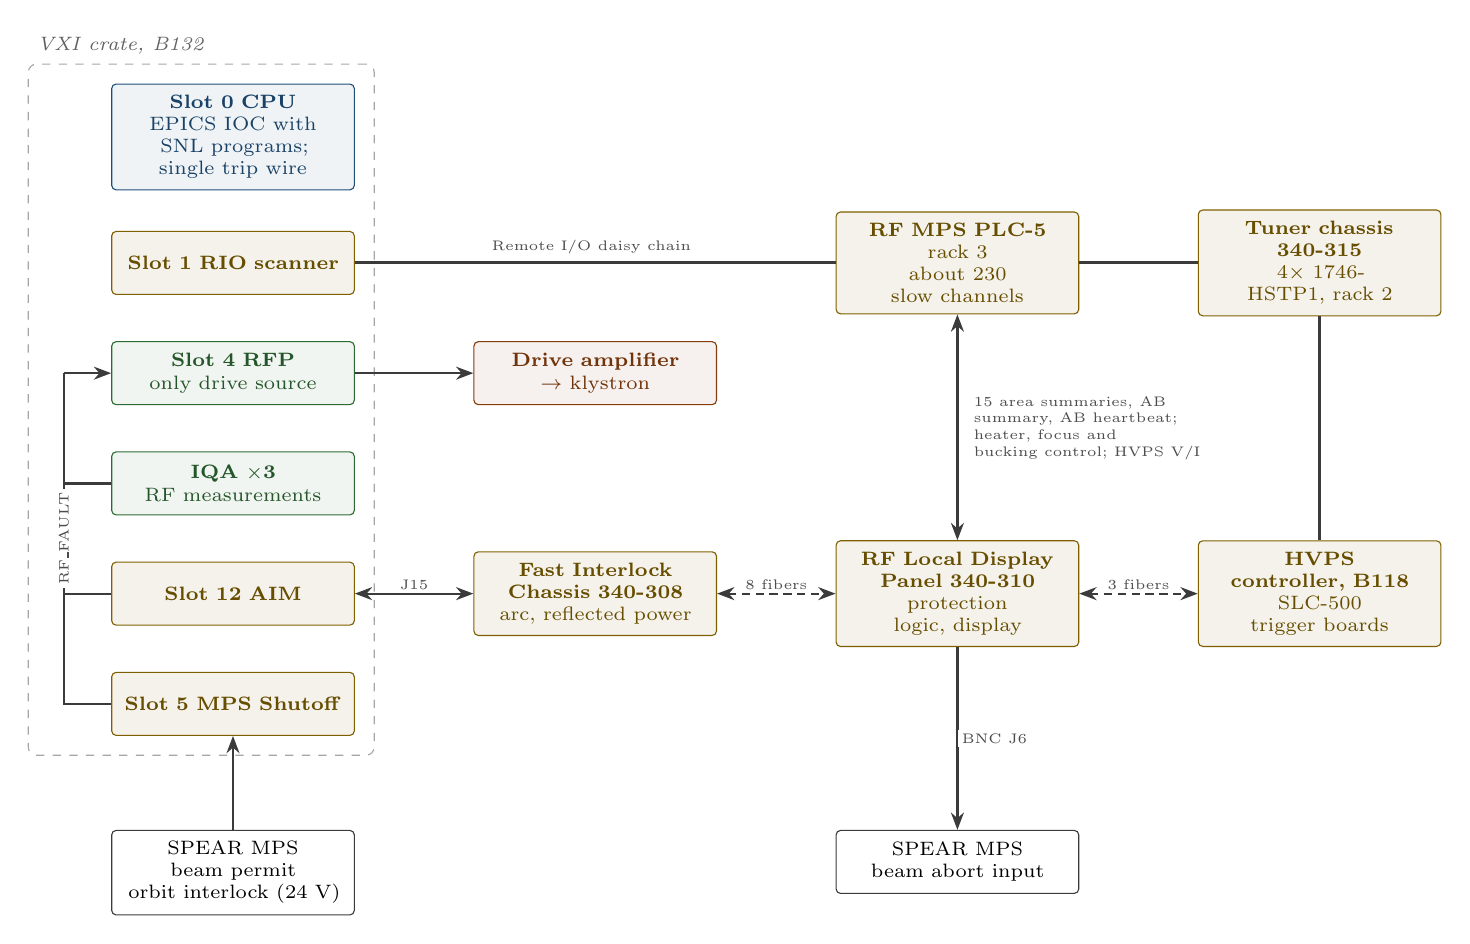
\begin{tikzpicture}[font=\scriptsize, x=1mm, y=1mm,
  every node/.append style={execute at begin node=\hyphenpenalty 10000\relax}]

% ----- VXI crate (column 1) ----------------------------------------------
\node[ctrl,text width=28mm,anchor=west] (cpu) at (10,-4)
  {\textbf{Slot 0 CPU}\\ EPICS IOC with\\ SNL programs;\\ single trip wire};
\node[plc,text width=28mm,anchor=west] (scn) at (10,-20)
  {\textbf{Slot 1 RIO scanner}};
\node[rf,text width=28mm,anchor=west]  (rfp) at (10,-34)
  {\textbf{Slot 4 RFP}\\ only drive source};
\node[rf,text width=28mm,anchor=west]  (iqa) at (10,-48)
  {\textbf{IQA $\times$3}\\ RF measurements};
\node[plc,text width=28mm,anchor=west] (aim) at (10,-62)
  {\textbf{Slot 12 AIM}};
\node[plc,text width=28mm,anchor=west] (s5)  at (10,-76)
  {\textbf{Slot 5 MPS Shutoff}};
% a real node, so that the crate outline also encloses the RF_FAULT lane
\node[inner sep=0pt,minimum size=0pt] (lane) at (2,-50) {};
\node[grp,fit=(cpu)(scn)(rfp)(iqa)(aim)(s5)(lane)] (crate) {};
\node[lbl,anchor=south west] at (crate.north west) {VXI crate, B132};

% RF_FAULT: open-collector backplane line; every fast RF-off path ends here
\draw[thick,draw=cNeut] (s5.west) -- (s5.west -| 4,0) -- (rfp.west -| 4,0);
\draw[thick,draw=cNeut] (aim.west) -- (aim.west -| 4,0);
\draw[thick,draw=cNeut] (iqa.west) -- (iqa.west -| 4,0);
\draw[sig] (rfp.west -| 4,0) -- (rfp.west);
\node[tag,rotate=90] at (4,-55) {RF\_FAULT};

% ----- column 2 -----------------------------------------------------------
\node[pwr,text width=28mm,anchor=west] (drv) at (56,-34)
  {\textbf{Drive amplifier}\\ $\rightarrow$ klystron};
\node[plc,text width=28mm,anchor=west] (fic) at (56,-62)
  {\textbf{Fast Interlock}\\ \textbf{Chassis 340-308}\\ arc, reflected power};

% ----- column 3 -----------------------------------------------------------
\node[plc,text width=28mm,anchor=west] (mps) at (102,-20)
  {\textbf{RF MPS PLC-5}\\ rack 3\\ about 230 slow channels};
\node[plc,text width=28mm,anchor=west] (lp)  at (102,-62)
  {\textbf{RF Local Display}\\ \textbf{Panel 340-310}\\ protection logic, display};

% ----- column 4 -----------------------------------------------------------
\node[plc,text width=28mm,anchor=west] (tun) at (148,-20)
  {\textbf{Tuner chassis 340-315}\\ 4$\times$ 1746-HSTP1, rack 2};
\node[plc,text width=28mm,anchor=west] (hv)  at (148,-62)
  {\textbf{HVPS controller, B118}\\ SLC-500\\ trigger boards};

% ----- external permits ---------------------------------------------------
\node[blk,text width=28mm,anchor=north] (ext) at (s5.south |- 0,-92)
  {SPEAR MPS beam permit\\ orbit interlock (24 V)};
\draw[sig] (ext.north) -- (s5.south);
\node[blk,text width=28mm,anchor=north] (bab) at (lp.south |- 0,-92)
  {SPEAR MPS\\ beam abort input};
\draw[sig] (lp.south) -- (bab.north);
\node[tag,anchor=west] at ($(lp.south)!0.5!(bab.north)$) {BNC J6};

% ----- Remote I/O daisy chain: scanner, PLC-5, tuner chassis, HVPS PLC ----
\draw[bus] (scn.east) -- (mps.west);
\draw[bus] (mps.east) -- (tun.west);
\draw[bus] (tun.south) -- (hv.north);
\node[tag,anchor=south] at (71,-19.4) {Remote I/O daisy chain};

% ----- RF drive ------------------------------------------------------------
\draw[sig] (rfp.east) -- (drv.west);

% ----- protection row -------------------------------------------------------
\draw[{Stealth[length=2.2mm]}-{Stealth[length=2.2mm]},thick,draw=cNeut]
  (aim.east) -- (fic.west);
\draw[{Stealth[length=2.2mm]}-{Stealth[length=2.2mm]},thick,draw=cNeut,densely dashed]
  (fic.east) -- (lp.west);
\draw[{Stealth[length=2.2mm]}-{Stealth[length=2.2mm]},thick,draw=cNeut,densely dashed]
  (lp.east) -- (hv.west);
\node[tag,anchor=south] at ($(aim.east)!0.5!(fic.west)$) {J15};
\node[tag,anchor=south] at ($(fic.east)!0.5!(lp.west)$) {8 fibers};
\node[tag,anchor=south] at ($(lp.east)!0.5!(hv.west)$) {3 fibers};

% ----- PLC-5 to RF Local Display Panel --------------------------------------
\draw[{Stealth[length=2.2mm]}-{Stealth[length=2.2mm]},thick,draw=cNeut]
  (mps.south) -- (lp.north);
\node[tag,anchor=west,align=left] at (119,-41)
  {15 area summaries, AB\\ summary, AB heartbeat;\\ heater, focus and\\ bucking control; HVPS V/I};
\end{tikzpicture}

\end{fitpicture}
\caption[Couplings of the legacy station.]{Couplings of the legacy station, with the
racks of \cref{tab:racks}. The Remote I/O link is one daisy chain from the VXI scanner
through the RF MPS PLC-5 and the tuner chassis to the HVPS controller. Every fast
RF-off path ends on the RFP through the open-collector backplane line RF\_FAULT. The
AIM, the Fast Interlock Chassis, the RF Local Display Panel and the HVPS controller
form one hardwired protection chain; the panel's logic forms SCR ENABLE, KLYSTRON
CROWBAR and a beam abort on BNC J6, which is not cabled. The Fast Interlock Chassis also
takes the twelve arc-detector fibers and holds the klystron forward-power detector,
with the RF in on J32 and the level out on J31 to an analog input of the PLC-5. The
PLC-5 controls the filament heater
and the focus and bucking coil supplies; the coil-supply faults also enter the panel's
logic. Dashed arrows are fibers.}\label{fig:legacy-couplings}
\end{figure}

\subsection{The Remote I/O Chain}\label{sec:rio}

The VXI slot-1 Allen-Bradley 6008-SV1R scanner, mounted through an HP E1407A adapter,
is the master of a single RIO link \R{2}. Its configuration addresses the three PLCs as
logical racks \R{11}, \R{32}; this plan names them after their devices
(\cref{tab:rio}).

\begin{longtable}[c]{@{}Q{\cw{0.14}{1.6}}Q{\cw{0.15}{1.6}}Q{\cw{0.50}{1.6}}Q{\cw{0.17}{1.6}}@{}}
\caption{Nodes of the legacy RIO link.}\label{tab:rio}\\
\toprule
Node & Logical rack & Device and adapter & Physical rack \\
\midrule
\endfirsthead
\toprule
Node & Logical rack & Device and adapter & Physical rack \\
\midrule
\endhead
\bottomrule
\endlastfoot
PLC-5 node & 3 & RF MPS PLC-5 through a 1771-DCM; first node & B132-13 \\
Tuner node & 2 & SLC-500 tuner chassis 340-315 with four 1746-HSTP1 modules;
middle node & B132-13 \\
HVPS node & 1 & HVPS SLC-500 through a 1747-DCM; last node & B118 \\
\end{longtable}

The chain runs from the scanner to the DCM in the main PLC-5 crate, on to the tuner
chassis and, through a terminal box above the HVPS termination tank, to the HVPS
SLC-500 in B118; the second PLC-5 crate hangs on the main crate's own link \R{6}.
Consequences:
\begin{itemize}
\item Every PLC datum and command reaches EPICS only through this chain and
\mbox{B132-IOCRF}.
\item A powered-down node loses only its own data, but disconnecting a node's
terminals cuts every node downstream: replacing the PLC-5 or the tuner chassis means
splicing the chain through, and removing the HVPS node means moving the terminating
resistor.
\item The PLC-5 node and the HVPS node behave differently when they stop answering.
The DCM record that reads the PLC-5 never reprocesses its records on a link change,
because its LOCA field is not set: while the IOC runs, the PLC-5 values freeze, the
adapter and DCM records go to MAJOR, the station status shows HWERROR and nothing
trips; after an IOC reboot without the node the PLC-5 records stay undefined and the
state machine refuses to turn the station on. The scanner driver instead sends the
HVPS records to INVALID, which turns the station off \R{42}. The PLC-5 itself does not
depend on the link (\cref{sec:plc5prog}), so its node can be taken off with the IOC
running, as the I4 entry test does (\cref{sec:i-mps}); the node's records are then
re-pointed as in \cref{sec:legacyioc}.
\end{itemize}

\subsection{The Hardwired Protection Chain}\label{sec:hwchain}

The chain is documented at the level of connectors and fibers in J.~Sebek's notes
\R{6}, \R{34} and in the original drawings \R{26}--\R{30}; Doc~C gives every line
\R{45}:
\begin{itemize}
\item \textbf{Fast Interlock Chassis 340-308.} J15, cabled to J3 of the AIM (VXI
slot~12), brings the AIM's six commands---FILAMENT\_ON (filament and focus request),
SOLENOID\_ON (station online request), HVPS\_ON, BEAM\_ABORT, FILAMENT\_TIMEOUT and
FAULT\_RESET---which the chassis turns into fibers to the panel, and returns the AB
summary and heartbeat from the panel \R{6}, \R{28}. The chassis also holds the
klystron forward-power detector for the PLC-5 (RF in on J32, level out on J31), an
arc-detection front end whose 37-pin J2 is cabled to the AIM's J4, and a spare-fault
input cabled to J3 of VXI Slot~5, which the AIM reads as its External MPS channel
\R{6}, \R{27}.
\item \textbf{RF Local Display Panel 340-310.} Eleven fibers: the six commands and
the AB summary and heartbeat to and from the Fast Interlock Chassis \R{29}, and three
to and from the HVPS controller. Its connectors J2 and J3, wired to cross-connect X530
in rack B132-14, carry the AIM's requests to the PLC-5, the PLC-5's summaries, AB
summary and heartbeat, and the HVPS voltage and current that the panel buffers for
the PLC-5's collector-power calculation \R{6}, \R{7}, \R{30}. The panel carries the
station online/offline and
local/remote key switches \R{26}.
\item \textbf{The panel's logic.} A GAL22V10 forms SCR ENABLE, KLYSTRON CROWBAR and
the beam abort from the HVPS-on request, the VXI and HVPS beam aborts, the online key
switch and the PLC-5's main-focus, bucking-coil, waveguide air-pressure and
collector-power summaries \R{38}; two flip-flops latch the beam abort and the crowbar
until reset \R{26}, \R{34}. Its equations are not documented, so the Interface
Chassis does not copy them (O1).
\item \textbf{HVPS fibers.} Three fibers run between the panel and the trigger
interconnect boards of the active HVPS controller in B118, through a switchbox that
selects the unit \R{6}, \R{29}, \R{31}, \R{34}: SCR ENABLE (lit to enable) and
KLYSTRON CROWBAR (lit for no crowbar) to the controller, and STATUS back, lit while
the controller's ``24~V fault/enable'' output is high and no crowbar is commanded;
the panel receives STATUS as the ``HVPS beam abort'' \R{4}, \R{26}.
\item \textbf{Arc triggers in the HVPS controller.} A Pearson current transformer in
the termination tank feeds the klystron-arc trigger input of the Left Side board, and
the transformer-arc trigger enters the Right Side board. Either one fires the crowbar
and inhibits the triggers in hardware; the SLC-500 only latches both as status bits
\R{4}, \R{5}, \R{14}, \R{25}. The panel sees them only as a dark STATUS fiber.
\item \textbf{VXI Slot~5 (``MPS Shutoff'').} The SPEAR MPS beam permit and the orbit
interlock (\qty{24}{\volt} each) \R{3}; dropping either asserts RF\_FAULT \R{2}. Its
J3 output drives the spare-fault input of the Fast Interlock Chassis, which the AIM
holds as its External MPS channel. The module and its wiring are traced under O6.
\item \textbf{RF\_FAULT.} An open-collector VXI backplane line. The AIM, the IQAs,
Slot~5, the CLK module and the RFP can assert it; the RFP then removes the drive
\R{2}.
\end{itemize}

\paragraph{Beam abort.} The state machine forces a beam abort through the AIM whenever
it turns the station off, enters TUNE or switches the direct loop, and resets it when
the station reaches ON\_CW with no faults \R{17}. The panel combines it with STATUS and
its other inputs and drives J6, an output made for the PEP-II beam-abort system \R{46}
that is not cabled at SPEAR3; the SPEAR MPS takes no status from the RF in hardware
and dumps the beam by removing the RF permit through Slot~5 \R{3}. The beam abort
therefore stays inside the station.

\begin{warnbox}
Every fast RF-off path of the legacy station ends on the RFP. High voltage is removed
in hardware through the panel's SCR ENABLE and KLYSTRON CROWBAR fibers or inside the
HVPS controller. A SPEAR MPS or orbit trip reaches the HVPS only through the RF cut and
the state machine, unless the PLC-5's collector-power protection acts first: after any
trip the state machine spends about \qty{1}{\second} in TUNE and \qty{5}{\second}
ramping the HVPS down before it removes the triggers and the RF switch \R{17}.
\end{warnbox}

\subsection{The RF Drive and Measurement Path}\label{sec:rfpath}

\begin{itemize}
\item The RFP is the only drive source. The 2021 cable record lists the RFP output and
the drive-amplifier input as separate, marked patch cables next to the LLRF9
reference, which came from output RF3 of the VXI CLK module \R{8}: the drive source
is selected by a patch cable.
\item The three IQA modules measure the 24 RF signals. The legacy loops and alarms use
their data: drive power for the HVPS loop, probe and forward phases for the tuner
loops, and reflected and forward powers for the alarms.
\item In 2021, \qty{20}{\decibel} couplers with about \qty{0.4}{\decibel} insertion
loss were inserted upstream of the legacy system for the nine signals the LLRF9
monitored---klystron forward, cavity forward and cavity probes---and the legacy
calibration constants were changed to compensate \R{9}.
\end{itemize}

\subsection{The Supervisory IOC B132-IOCRF}\label{sec:ioc}

\begin{itemize}
\item The VXI slot-0 processor runs the IOC \mbox{B132-IOCRF} under vxWorks. It loads
one expanded database, \fpath{srf1.db}, restores saved settings, configures the RIO
scanner from \fpath{config.ab} and starts nine SNL program instances: the state
machine, four tuner loops, the HVPS loop, the DAC loop, a calibration sequence and the
message logger \R{10}. It stays the station IOC and the coordinator, and moves to new
hardware at I8.
\item The state machine trips on one summary, \fpath{SRF1:STNOFF:SUMY:STAT}. It
collects the VXI latch, the HVPS off summary, the PLC-5's online bit (the panel's
online key and the station-online command), the AB summary latch and the PLC-5's own
station summary bit; turn-on
is blocked by a similar summary, \fpath{SRF1:STNON:SUMY:STAT} \R{17}, \R{19}. Cavity,
tuner and temperature alarms reach only the station status display.
\item A database change is a text edit and a reboot. An SNL change needs the EPICS
3.14.11 vxWorks cross-development environment, whose availability is not
confirmed.\openitem{O5} The release was built on Solaris for vxWorks~5.4, in AFS and
later in NFS, and its last changes, in 2021, were to the database only \R{43}.
\item The SNL bindings that matter for the integrations, among them the HVPS loop's
dependence on the RFP \R{16}, are listed in Appendix~\ref*{app:epics}.
\end{itemize}

\subsection{Data the PLC-5 Provides to Other Subsystems}\label{sec:plc5data}

The PLC-5 is the station's slow data system as well as an equipment-protection PLC.
About 230 template instances in the legacy database take their data from it
(Appendix~\ref*{app:epics}): about 110 temperatures, about 40 interlock bits, about 30
analog channels and about 50 summary, module and digital status points \R{13},
\R{14}. Several belong to other subsystems: the tuner potentiometer positions
(\fpath{SRF1:CAVnTUNR:POSN}) and temperatures; the stepper drivers' bulk supply
voltage (\fpath{SRF1:CAVTUNR:VOLT}), whose latch feeds the tuner summary \R{13},
\R{19}; filament voltage and current with their PLC-5 trip limits, and the main focus
and bucking-coil supply voltages and currents; klystron and circulator ion-pump
currents and window temperatures; and the HVPS voltage and current as seen by the PLC
(the collector-power inputs) and the HVPS oil temperature \R{12}. Every integration
that touches the PLC-5, the tuner, the heater or the HVPS checks these channels.

\subsection{The RF MPS Program}\label{sec:plc5prog}

Four RSLogix~5 projects of the PLC-5 program---an undated one with the address
descriptions and edits saved in November 2011 and February 2012---have been decoded
into readable listings \R{38}. Their logic is the same apart from two limit changes.
The 2021 filament changes are not in them, so the program in service has to be
uploaded and compared (O8). The program shows:
\begin{itemize}
\item \textbf{EPICS link.} The PLC-5 writes eight 64-word pages to the DCM in turn;
word~3 of each page holds the page number, which is the table number that the legacy
records address. A page is resent after a transfer error, and the block read back from
the DCM is used by no rung. Nothing in the program depends on the link, so the PLC-5
runs the same with or without the IOC.
\item \textbf{Global interlock sum.} One bit is both the station summary that EPICS
reads (\fpath{SRF1:STN:SUMY:PLC}) and the AB summary line to the AIM. It requires the
four cavity summaries, the waveguide-load, waveguide air-pressure and circulator
summaries, an input labeled ``MPS'' on the drawings, and---while the online bit
(\fpath{SRF1:STN:LOCAL:ON}, the online/offline-mode and klystron-focusing lines both
on) is set---the klystron group (klystron water, temperatures, vacuum and air flow;
filament; focus; collector power) and the flow, vacuum and temperature summaries.
Every fault latches until the panel's reset line, once its condition has cleared.
\item \textbf{Heartbeat.} A \qty{50}{\milli\second} timer turns the heartbeat output
on for one scan each time it expires. It stops when any of the 16 analog and
thermocouple modules reports a read error, until reset; the DCM is not involved.
\item \textbf{Collector power.} The beam power from the HVPS voltage and current
buffered by the panel, minus the RF output power from the forward-power detector input
``RF PWR LEVEL'' \R{41}, trips above \qty{1200}{\kilo\watt} for
\qty{0.7}{\second}. HV detected and RF detected are thresholds on the same inputs, at
about \qty{9.7}{\kilo\volt} and \qty{9}{\kilo\watt}.
\item \textbf{Filament.} The warm-up sequence of \cref{sec:i-heater}, the trips on the
heater voltage and current, and the window-air blower, which runs while the filament
is on and for \qty{600}{\second} after.
\item \textbf{Cavity vacuum.} The analog cavity-vacuum readings trip on eight
pressure steps with delays from \qty{900}{\second} down to \qty{1}{\second}; these
trips latch bits that only EPICS reads and are not in the global sum.
\end{itemize}

% ===========================================================================
\section{Integration Plan}\label{sec:plan}

\subsection{Sequence}\label{sec:sequence}

The project has set the order of the integrations (\cref{tab:sequence});
\cref{fig:sequence} shows which links in the order are technical and which are only
planned. The Interface Chassis (I2) gives the ARC4 its trip input and the LLRF9 its
enable, so neither needs an interim path in the legacy chain. HVPS control passes to
the LLRF9 on the legacy controllers (I7a), which sets the baseline for the new
controllers; these (I7b, I7c) wait for the PPS approval.

\begin{longtable}[c]{@{}Q{\cw{0.06}{1.6}}Q{\cw{0.20}{1.6}}Q{\cw{0.17}{1.6}}Q{\cw{0.34}{1.6}}Q{\cw{0.23}{1.6}}@{}}
\caption{Integration sequence.}\label{tab:sequence}\\
\toprule
Step & Integration & Replaces & Hard prerequisites & Fallback \\
\midrule
\endfirsthead
\toprule
Step & Integration & Replaces & Hard prerequisites & Fallback \\
\midrule
\endhead
\bottomrule
\endlastfoot
I0 & Preparation (\cref{sec:i0}) & --- & --- & --- \\
I1 & ARC4 and LLRF9 measurement, monitor-only (\cref{sec:i-monitor}) & Disconnected
optical arc front end & Arc fibers checked (O3); LLRF9 hookup as a controlled change;
SW8 & None needed \\
I2 & Interface Chassis and Waveform Buffer (\cref{sec:i-ic}) & Fast Interlock Chassis;
RF Local Display Panel & Production unit with the transition interfaces; O1 to O4 and
O7; SW7; baseline test of the legacy chain; failure-mode analysis & Reinstall the Fast
Interlock Chassis and the panel \\
I3 & Tuner control by LLRF9 Unit~1 and the Galil (\cref{sec:i-tuner}) & 1746-HSTP1
tuner control & I1; SW2; legacy tuner loops off with their alarms adjusted & Motor
cables back to the SS2000 drivers \\
I4 & RF MPS (\cref{sec:i-mps}) & PLC-5 & Legacy-faithful program (O8); SW1 and SW5;
legacy database change; RIO splice; trip test & PLC-5 \\
I5 & Klystron heater supply under RF MPS control (\cref{sec:i-heater}) & Variac stage
& I4; \qty{60}{\hertz} sync circuit; SW3; acceptance on the test stand; a long down &
Variac chassis \\
I6 & LLRF9 as drive source (\cref{sec:i-drive}) & RFP as drive source & I2; SW9; O5
and O6; interlocked RF transfer switch & Transfer switch to the RFP \\
I7a & HVPS control by the LLRF9 on the legacy controllers (\cref{sec:i-hvps-a}) & The
legacy HVPS loop, if I6 kept it & I6; SW9 & The configuration of I6 \\
I7b & First new HVPS controller and PPS Interface Box (\cref{sec:i-hvps-b}) & Hoffman
box of the off-duty unit and its PPS wiring & I7a; ADSO approval; PPS certification;
the new box run on Test Stand~18; SW6; O9 & Switch-over to the legacy unit \\
I7c & Second new HVPS controller and PPS Interface Box (\cref{sec:i-hvps-c}) &
Hoffman box of the other unit and its PPS wiring & I7b, with months of operation
without a controller fault & The first new unit \\
I8 & Legacy retirement (\cref{sec:i-retire}) & VXI crate; RIO link; tuner chassis &
I1 to I7c, both HVPS units on new boxes; SW10 on the new hardware of
\mbox{B132-IOCRF}; reference distribution; a home for every legacy function & None
practical \\
\end{longtable}

\begin{figure}[tbp]
\centering
\begin{fitpicture}
% !TeX root = ../M_integration_migration_plan.tex
% Stage dependencies.  Column 2 is ordered so that the two inputs of the S6
% join (S4 and the minimal coordinator) are adjacent: every other line then
% passes clear of that join bar.  Bars (thick vertical lines) mean "all of".
%   col 1 S0 0-30.8, spine x = 38; col 2 44-86.8; S6 join x = 94;
%   S6 102-132.8; S7 join x = 142; S7 150-180.8.
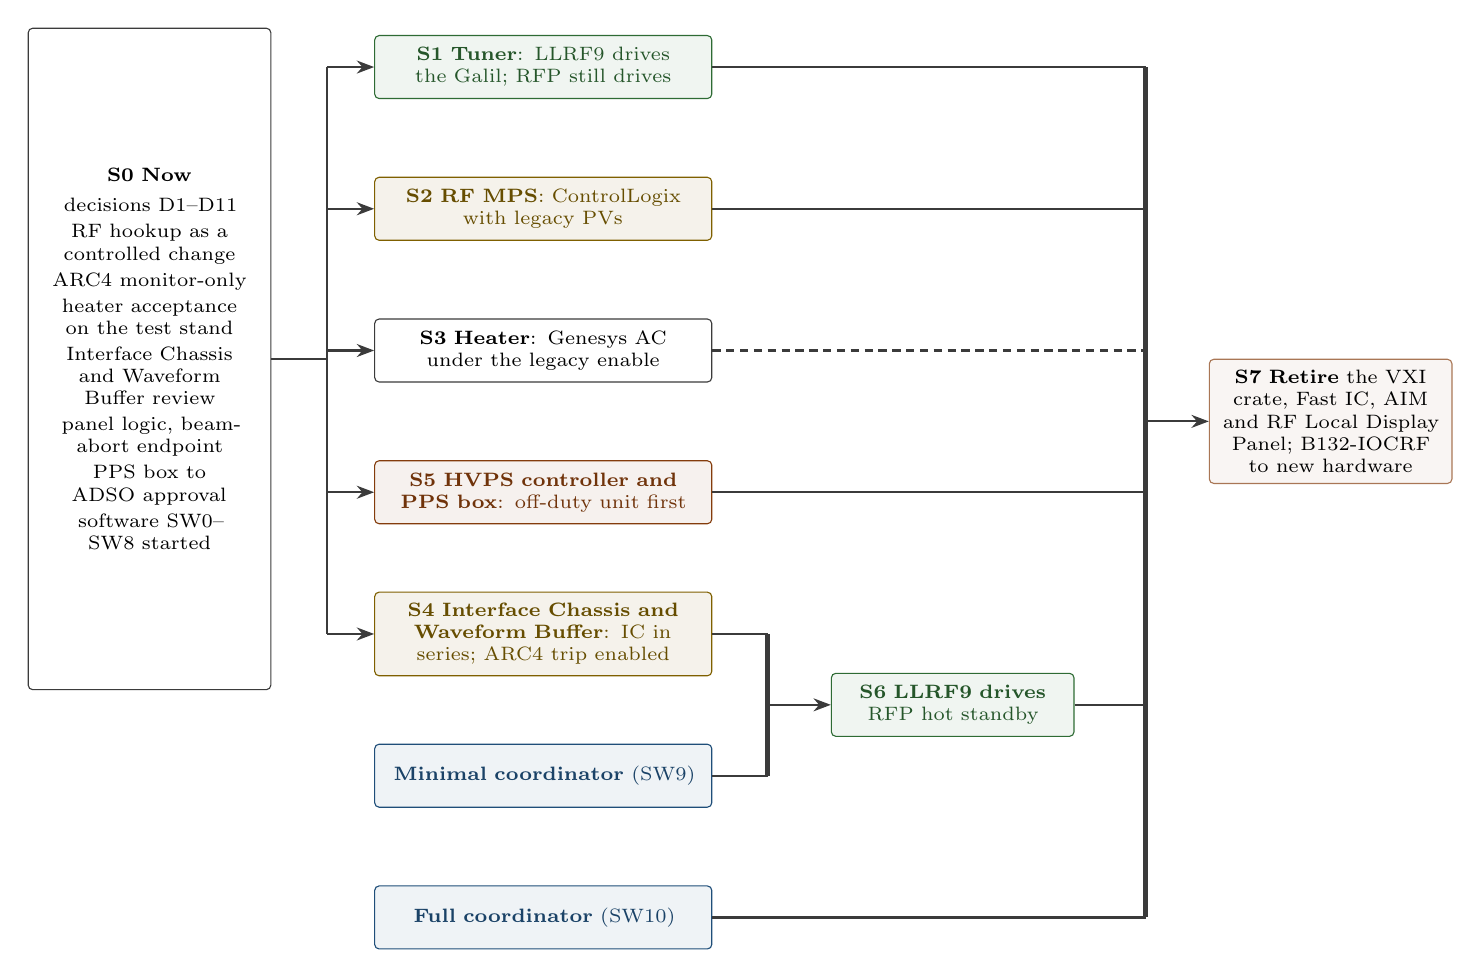
\begin{tikzpicture}[font=\scriptsize, x=1mm, y=1mm,
  every node/.append style={execute at begin node=\hyphenpenalty 10000\relax}]

% ----- column 2: the independent stages and the two software releases ------
\node[rf,  text width=40mm,anchor=west] (s1)   at (44,0)
  {\textbf{S1 Tuner}: LLRF9 drives the Galil; RFP still drives};
\node[plc, text width=40mm,anchor=west] (s2)   at (44,-18)
  {\textbf{S2 RF MPS}: ControlLogix with legacy PVs};
\node[blk, text width=40mm,anchor=west] (s3)   at (44,-36)
  {\textbf{S3 Heater}: Genesys AC under the legacy enable};
\node[pwr, text width=40mm,anchor=west] (s5)   at (44,-54)
  {\textbf{S5 HVPS controller and PPS box}: off-duty unit first};
\node[plc, text width=40mm,anchor=west] (s4)   at (44,-72)
  {\textbf{S4 Interface Chassis and Waveform Buffer}: IC in series; ARC4 trip enabled};
\node[ctrl,text width=40mm,anchor=west] (sw9)  at (44,-90)
  {\textbf{Minimal coordinator} (SW9)};
\node[ctrl,text width=40mm,anchor=west] (sw10) at (44,-108)
  {\textbf{Full coordinator} (SW10)};

% ----- column 1: stage 0 feeds every independent stage ---------------------
\node[blk,text width=28mm,minimum height=84mm,anchor=north west] (s0) at (0,5)
  {\textbf{S0 Now}\\[1mm]
   decisions D1--D11\\[0.5mm]
   RF hookup as a controlled change\\[0.5mm]
   ARC4 monitor-only\\[0.5mm]
   heater acceptance on the test stand\\[0.5mm]
   Interface Chassis and Waveform Buffer review\\[0.5mm]
   panel logic, beam-abort endpoint\\[0.5mm]
   PPS box to ADSO approval\\[0.5mm]
   software SW0--SW8 started};
\draw[thick,draw=cNeut] (38,0) -- (38,-72);
\draw[thick,draw=cNeut] (s0.east) -- (s0.east -| 38,0);
\foreach \n in {s1,s2,s3,s5,s4}{\draw[sig] (\n.west -| 38,0) -- (\n.west);}

% ----- S6: needs the Interface Chassis AND the minimal coordinator ---------
\node[rf,text width=28mm,anchor=west] (s6) at (102,-81)
  {\textbf{S6 LLRF9 drives}\\ RFP hot standby};
\draw[thick,draw=cNeut] (s4.east)  -- (s4.east -| 94,0);
\draw[thick,draw=cNeut] (sw9.east) -- (sw9.east -| 94,0);
\draw[line width=1.8pt,draw=cNeut] (94,-72) -- (94,-90);
\draw[sig] (94,-81) -- (s6.west);

% ----- S7: needs all of S1, S2, S5, S6 and the full coordinator ------------
\node[blk,text width=28mm,anchor=west,draw=cPwr!70,fill=cPwr!5] (s7) at (150,-45)
  {\textbf{S7 Retire} the VXI crate, Fast IC, AIM and RF Local Display Panel;
   B132-IOCRF to new hardware};
\draw[line width=1.8pt,draw=cNeut] (142,0) -- (142,-108);
\draw[thick,draw=cNeut] (s1.east)   -- (s1.east -| 142,0);
\draw[thick,draw=cNeut] (s2.east)   -- (s2.east -| 142,0);
\draw[thick,draw=cNeut,densely dashed] (s3.east) -- (s3.east -| 142,0);
\draw[thick,draw=cNeut] (s5.east)   -- (s5.east -| 142,0);
\draw[thick,draw=cNeut] (s6.east)   -- (s6.east -| 142,0);
\draw[thick,draw=cNeut] (sw10.east) -- (sw10.east -| 142,0);
\draw[sig] (142,-45) -- (s7.west);
\end{tikzpicture}

\end{fitpicture}
\caption[Integration sequence.]{Integration sequence. Solid arrows are technical
prerequisites, dashed arrows only the planned order; I6 runs in parallel with I4 and
I5.}\label{fig:sequence}
\end{figure}

\subsection{Rules for Every Integration}\label{sec:rules}

\begin{enumerate}
\item \textbf{Legacy names are the interface.} A replacement keeps the PV names,
units, scaling and alarm limits of the records it replaces until the full coordinator
takes over; the HVPS keeps its names for good.
\item \textbf{No new permits.} A new element in a permit path can remove a permit but
never create one. Where it generates a permit itself, as the Interface Chassis does
from I2 on, a failure-mode analysis and an equivalence test against the recorded
legacy behavior come first.
\item \textbf{Monitor-only first} for a run period, where the subsystem allows it.
\item \textbf{One integration per window}, so that any new behavior has one cause; two
integrations that need the same person are not scheduled in the same window.
\item \textbf{Tested fallback.} A written fallback procedure is tested before the
window, and the legacy hardware stays intact until the next integration has run
without it.
\item \textbf{Configuration control.} Every hybrid configuration is recorded:
connections, calibration constants, database version, jumpers and bypasses.
\end{enumerate}

% ===========================================================================
\section{Integration Requirements}\label{sec:reqs}

Each integration is described under the same headings: scope; interfaces to the legacy
station; a worklist of hardware, software and tests; entry criteria; fallback. The
software work packages SW0 to SW10 are listed in \cref{tab:wp}.

% ---------------------------------------------------------------------------
\subsection{I0: Preparation}\label{sec:i0}

Alongside the first integrations, without effect on beam (\cref{tab:wl-i0}). The
baselines of I0-T1 and I0-T3 are the references against which I2 and I4 are accepted.
In every worklist, H marks hardware, S software and T tests and records; the last
column names the open items, work packages and other items each one depends on.

\begin{longtable}[c]{@{}Q{\cw{0.10}{1.333}}Q{\cw{0.70}{1.333}}Q{\cw{0.20}{1.333}}@{}}
\caption{Worklist of I0.}\label{tab:wl-i0}\\
\toprule
Item & Work & Depends on \\
\midrule
\endfirsthead
\toprule
Item & Work & Depends on \\
\midrule
\endhead
\bottomrule
\endlastfoot
I0-H1 & Production review of the Interface Chassis and the Waveform Buffer with the
requirements of \cref{sec:i-ic} and Doc~C \R{45} (A6) & O1 to O4 \\
I0-S1 & Decisions D1 to D11 recorded (A1); PV naming policy, legacy compatibility
rules and one interface control document per integration (SW0) & --- \\
I0-S2 & Legacy IOC owner named; test IOC set up; procedure to edit, build and reload
\fpath{srf1.db} written and rehearsed; SNL build checked (SW1, A2) & O5 \\
I0-S3 & The LLRF9 vendor software of April 2026 reviewed on a spare unit: its links
to legacy PVs, which carry the prefix SRFTEST, its HVPS loop, tuner interfaces and
state machine \R{39} (A17) & O7 \\
I0-T1 & Baseline of the legacy protection chain: the panel's response to every input
that can be set without high voltage, the three HVPS
fibers, the HVPS controller's arc triggers as seen on STATUS, the heartbeat at the
panel and at the AIM, the request line at X530 that each AIM command drives, and the
AIM's HVPS-on request and SCR ENABLE through a turn-off and a forced fault (A3,
A5) & O4 \\
I0-T2 & The PLC-5 program in service uploaded and compared with the decoded 2012
program \R{38} (A16) & O8 \\
I0-T3 & The PLC-5 trip matrix run on the PLC-5 in service (A13) & I0-T2 \\
I0-T4 & Work that needs no window, started early: the Galil bench test (I3-T1), the
heater test-stand acceptance (I5-T1), the PPS box approval steps (A14) & --- \\
\end{longtable}

% ---------------------------------------------------------------------------
\subsection{I1: ARC4 and LLRF9 Measurement, Monitor-Only}\label{sec:i-monitor}

\paragraph{Scope.} The ARC4 and the two LLRF9 units go in with no output in any trip or
control path. The ARC4 has twelve detector modules---ten for the four cavity windows
(two fibers each), the klystron output window and the circulator, and two spares---and
two system modules and a test module form its external interface \R{1}. The optical
arc detectors at the cavity windows were never commissioned, and the arc front end of
the Fast Interlock Chassis is largely disconnected \R{3}, \R{6}; cavity arcs are caught
only through the reflected-power and cavity-field faults \R{5}, so there the ARC4 adds
protection. Klystron and HVPS transformer arcs are caught by the arc triggers in the
HVPS controller, which I1 and I2 do not touch (\cref{sec:hwchain}). Both LLRF9 units
are installed in B132-13; their RF cabling is to be completed.

\paragraph{Interfaces.}
\begin{itemize}
\item ARC4: the tunnel fibers, at the rear of the VXI crate and the Fast Interlock
Chassis today \R{2}, move to the ARC4 once none is found to feed a live AIM arc channel
(O3); its system-module outputs stay unconnected until I2.
\item LLRF9: taps and splitters on the legacy RF signals, reusing the 2021 couplers
where possible, and the reference from output RF3 of the VXI CLK module \R{8}. Each
LLRF9 needs the reference at $10 \pm 1$~dBm \R{40}; RF3 gave 12.2~dBm at the patch
panel in 2021, and a two-way split leaves about 8.8~dBm, so a reference amplifier is
added ahead of the split to both units and the Waveform Buffer \R{8}. The Waveform
Buffer taps of I2 follow I1-H3 and I1-T3.
\item LLRF9 software: the vendor software of April 2026 holds a channel map for each
unit and functions that write to other IOCs---an HVPS loop, a tuner interface to the
legacy steppers and a station state machine---none of which may act on the station in
I1 \R{39}. Unit~1 keeps the vendor map, which the field loop needs; Unit~2's map
follows the allocation of Doc~0, with the klystron drive in place of waveguide load~1
forward \R{1}.
\end{itemize}

\paragraph{Worklist.} \Cref{tab:wl-i1}.

\begin{longtable}[c]{@{}Q{\cw{0.10}{1.333}}Q{\cw{0.70}{1.333}}Q{\cw{0.20}{1.333}}@{}}
\caption{Worklist of I1.}\label{tab:wl-i1}\\
\toprule
Item & Work & Depends on \\
\midrule
\endfirsthead
\toprule
Item & Work & Depends on \\
\midrule
\endhead
\bottomrule
\endlastfoot
I1-H1 & ARC4 chassis installed in B132 with its detector, system and test modules; its
outputs left unconnected until I2 & Doc~0 O4 \\
I1-H2 & Tunnel arc fibers moved from the rear of the VXI crate and the Fast Interlock
Chassis to the ARC4, once none is found to feed a live AIM arc channel & O3, I1-T1 \\
I1-H3 & LLRF9 RF hookup as a controlled change: the 2021 couplers and splitters for
the nine signals of Unit~1; new taps for the klystron drive, the circulator-load
forward and the waveguide-load 2 and 3 forward signals of Unit~2; the reference from
CLK output RF3 to both units through an amplifier and a splitter, at
$10 \pm 1$~dBm into each; the patch-panel record updated (A8) & --- \\
I1-H4 & Both LLRF9 units on the controls network & --- \\
I1-S1 & SW8: vendor IOC of April 2026 with the control channel map on Unit~1 and the
monitor map on Unit~2, edited to the allocation of Doc~0 \R{1}, \R{39}; calibration
against the IQAs; screens, alarms, archiving
and the Channel Access gateway & I1-H3 \\
I1-S2 & Monitor-only safeguards in the vendor IOC: the HVPS loop in its open mode,
the tuner interfaces disabled, the station state machine not used, and no Channel
Access write from the LLRF9 to \mbox{B132-IOCRF} or to any SRFTEST name \R{39} & O7,
I0-S3 \\
I1-T1 & Light test of every arc fiber end to end at the next tunnel access (none has
been used in service); the ARC4 electronics exercised with its test module & --- \\
I1-T2 & Shadow comparison of the LLRF9 phases and amplitudes with the IQAs at several
beam currents, among them Unit~2's klystron drive against the IQA drive power that the
HVPS loop uses & I1-S1 \\
I1-T3 & IQA calibrations and protection thresholds rechecked after each tap & I1-H3
\\
I1-T4 & No legacy PV and no drive changes while the LLRF9 IOCs run, reboot and lose
the network & I1-S2 \\
\end{longtable}

\paragraph{Entry criteria.} I1-S2 in place; the arc fibers checked against live AIM
channels; the LLRF9 hookup planned as a controlled change with the threshold recheck.

\paragraph{Fallback.} None needed in a trip path; a removed tap is reversed with the
previous calibration constants.

% ---------------------------------------------------------------------------
\subsection{I2: Interface Chassis and Waveform Buffer in Place of the Fast Interlock
Chassis and the RF Local Display Panel}\label{sec:i-ic}

\paragraph{Scope.} The production chassis, with the Interface Chassis and Waveform
Buffer boards, replaces the Fast Interlock Chassis 340-308 and the RF Local Display
Panel 340-310 in one down (\cref{fig:after-ic}). The AIM, the RFP, the PLC-5, the
tuner chassis and the HVPS controllers stay in service, so the Interface Chassis must
work with each of them exactly as the two legacy units do. I2 is a replacement, not a
series insertion: from I2 on, the Interface Chassis itself generates SCR ENABLE
and KLYSTRON CROWBAR (rule~2 of \cref{sec:rules}). The ARC4, installed
at I1, is read in from the start; its trip is enabled after a logged run.

\begin{figure}[tbp]
\centering
\begin{fitpicture}
% !TeX root = ../M_integration_migration_plan.tex
% The station after integration I2: same grid as fig-legacy-couplings, with the
% Interface Chassis (and the Waveform Buffer in the same chassis) spanning
% columns 2 and 3 of the protection row, where the Fast Interlock Chassis and
% the RF Local Display Panel were.  Inputs used later (the ARC4 trip after a
% logged run; the LLRF9 enable and permits from I6 on) are dashed.
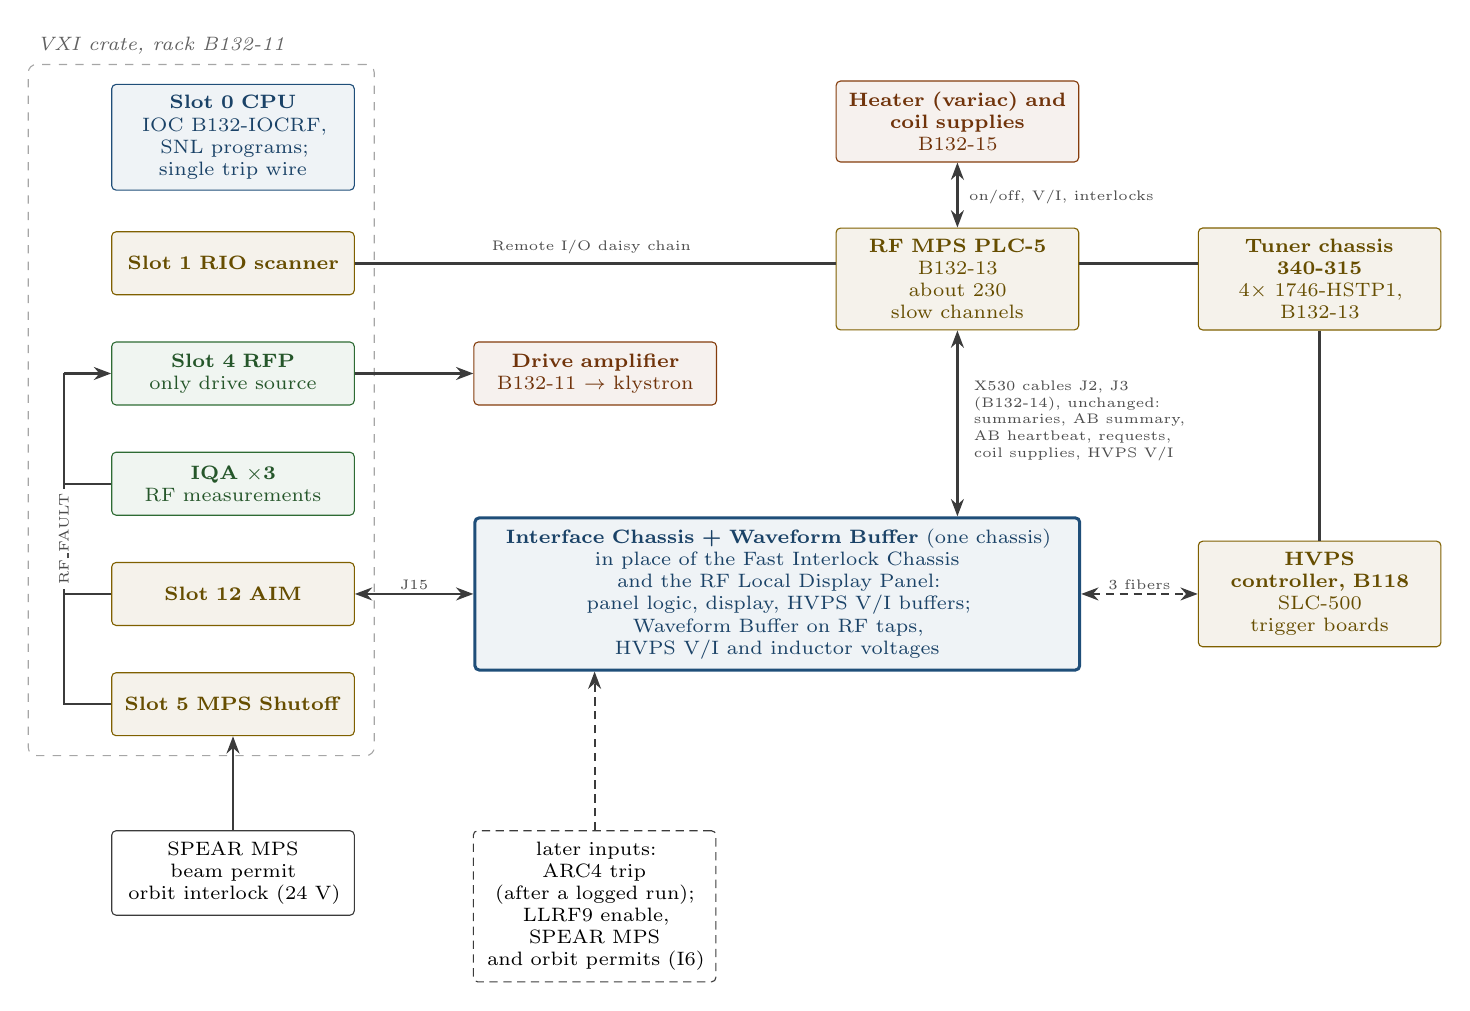
\begin{tikzpicture}[font=\scriptsize, x=1mm, y=1mm,
  every node/.append style={execute at begin node=\hyphenpenalty 10000\relax},
  new/.style={ctrl,line width=1.1pt}]

% ----- VXI crate (column 1), unchanged ------------------------------------
\node[ctrl,text width=28mm,anchor=west] (cpu) at (10,-4)
  {\textbf{Slot 0 CPU}\\ IOC B132-IOCRF,\\ SNL programs;\\ single trip wire};
\node[plc,text width=28mm,anchor=west] (scn) at (10,-20)
  {\textbf{Slot 1 RIO scanner}};
\node[rf,text width=28mm,anchor=west]  (rfp) at (10,-34)
  {\textbf{Slot 4 RFP}\\ only drive source};
\node[rf,text width=28mm,anchor=west]  (iqa) at (10,-48)
  {\textbf{IQA $\times$3}\\ RF measurements};
\node[plc,text width=28mm,anchor=west] (aim) at (10,-62)
  {\textbf{Slot 12 AIM}};
\node[plc,text width=28mm,anchor=west] (s5)  at (10,-76)
  {\textbf{Slot 5 MPS Shutoff}};
\node[inner sep=0pt,minimum size=0pt] (lane) at (2,-50) {};
\node[grp,fit=(cpu)(scn)(rfp)(iqa)(aim)(s5)(lane)] (crate) {};
\node[lbl,anchor=south west] at (crate.north west) {VXI crate, rack B132-11};

\draw[thick,draw=cNeut] (s5.west) -- (s5.west -| 4,0) -- (rfp.west -| 4,0);
\draw[thick,draw=cNeut] (aim.west) -- (aim.west -| 4,0);
\draw[thick,draw=cNeut] (iqa.west) -- (iqa.west -| 4,0);
\draw[sig] (rfp.west -| 4,0) -- (rfp.west);
\node[tag,rotate=90] at (4,-55) {RF\_FAULT};

% ----- unchanged boxes ------------------------------------------------------
\node[pwr,text width=28mm,anchor=west] (drv) at (56,-34)
  {\textbf{Drive amplifier}\\ B132-11 $\rightarrow$ klystron};
\node[pwr,text width=28mm,anchor=west] (htr) at (102,-2)
  {\textbf{Heater (variac) and}\\ \textbf{coil supplies}\\ B132-15};
\node[plc,text width=28mm,anchor=west] (mps) at (102,-22)
  {\textbf{RF MPS PLC-5}\\ B132-13\\ about 230 slow channels};
\node[plc,text width=28mm,anchor=west] (tun) at (148,-22)
  {\textbf{Tuner chassis 340-315}\\ 4$\times$ \mbox{1746-HSTP1}, B132-13};
\node[plc,text width=28mm,anchor=west] (hv)  at (148,-62)
  {\textbf{HVPS controller, B118}\\ SLC-500\\ trigger boards};

% ----- the new chassis -------------------------------------------------------
\node[new,text width=74mm,anchor=west] (ic) at (56,-62)
  {\textbf{Interface Chassis + Waveform Buffer} (one chassis)\\
   in place of the Fast Interlock Chassis and the RF Local Display Panel:\\
   panel logic, display, HVPS V/I buffers;\\
   Waveform Buffer on RF taps, HVPS V/I and inductor voltages};

% ----- external connections -------------------------------------------------
\node[blk,text width=28mm,anchor=north] (ext) at (s5.south |- 0,-92)
  {SPEAR MPS beam permit\\ orbit interlock (24 V)};
\draw[sig] (ext.north) -- (s5.south);
\node[blk,text width=28mm,anchor=north,densely dashed] (later) at (71.4,-92)
  {later inputs: ARC4 trip\\ (after a logged run);\\ LLRF9 enable, SPEAR MPS\\ and orbit permits (I6)};
\draw[sig,densely dashed] (later.north) -- (later.north |- ic.south);

% ----- Remote I/O daisy chain, unchanged ------------------------------------
\draw[bus] (scn.east) -- (scn.east -| mps.west);
\draw[bus] (mps.east |- 0,-20) -- (tun.west |- 0,-20);
\draw[bus] (tun.south) -- (hv.north);
\node[tag,anchor=south] at (71,-19.4) {Remote I/O daisy chain};

\draw[{Stealth[length=2.2mm]}-{Stealth[length=2.2mm]},thick,draw=cNeut]
  (htr.south) -- (mps.north);
\node[tag,anchor=west] at (118.4,-11.6) {on/off, V/I, interlocks};
\draw[sig] (rfp.east) -- (drv.west);

% ----- protection row through the Interface Chassis -------------------------
\draw[{Stealth[length=2.2mm]}-{Stealth[length=2.2mm]},thick,draw=cNeut]
  (aim.east) -- (ic.west);
\draw[{Stealth[length=2.2mm]}-{Stealth[length=2.2mm]},thick,draw=cNeut,densely dashed]
  (ic.east) -- (hv.west);
\node[tag,anchor=south] at ($(aim.east)!0.5!(ic.west)$) {J15};
\node[tag,anchor=south] at ($(ic.east)!0.5!(hv.west)$) {3 fibers};

\draw[{Stealth[length=2.2mm]}-{Stealth[length=2.2mm]},thick,draw=cNeut]
  (mps.south) -- (mps.south |- ic.north);
\node[tag,anchor=west,align=left] at (119,-40)
  {X530 cables J2, J3\\ (B132-14), unchanged:\\ summaries, AB summary,\\ AB heartbeat, requests,\\ coil supplies, HVPS V/I};
\end{tikzpicture}

\end{fitpicture}
\caption[The station after I2.]{The station after I2. The Interface Chassis, with the
Waveform Buffer in the same chassis, takes the place of the Fast Interlock Chassis and
the RF Local Display Panel and presents their interfaces to the AIM, the PLC-5 and the
HVPS controller, among them the RF cables J32 and J31 of the forward-power detector; it
takes the SPEAR MPS and orbit permits in parallel with Slot~5 and the ARC4, to which
the arc fibers moved at I1, and holds the LLRF9 enable on in place of the 2021 chassis
(O7). Everything else is as in \cref{fig:legacy-couplings}. Dashed: fibers, and the
inputs that act only after a logged run.}\label{fig:after-ic}
\end{figure}

\paragraph{Interfaces.} \Cref{tab:i1} lists what the Interface Chassis must present
at I2; these transition interfaces are in Doc~0 \R{1} but not in J.~Sebek's
specification \R{3}. Doc~C sets the design requirements \R{45}.

\begin{longtable}[c]{@{}Q{\cw{0.16}{1.333}}Q{\cw{0.32}{1.333}}Q{\cw{0.52}{1.333}}@{}}
\caption{Interfaces of the Interface Chassis at I2.}\label{tab:i1}\\
\toprule
Interface & Today & Requirement \\
\midrule
\endfirsthead
\toprule
Interface & Today & Requirement \\
\midrule
\endhead
\bottomrule
\endlastfoot
AIM, cable J15 & The Fast Interlock Chassis turns the AIM's six commands into fibers
and returns the AB summary and heartbeat \R{6} & Cable unchanged: five commands
received at today's levels, the beam abort on pin~15 not connected; the AB summary
(pin~10) and heartbeat (pin~23) driven; supply and trip-test pins not
connected\openitem{O3} \\
AIM, 37-pin cable to J4 & Twelve arc signals and, on pin~34, the spare-fault line from
Slot~5's J3, the AIM's External MPS channel; jumpers on the AIM enable the channels
(\texttt{0x71FB}, read 11 November 2026) \R{27}, \R{28} & Cable unchanged: pin~34 held
low while both machine permits are present; arc lines terminated at their no-arc
level; pins~35 to 37 not connected; Slot~5's J3 cable left open \R{45} \\
SPEAR MPS and orbit permits & Two \qty{24}{\volt} permits into VXI Slot~5, which
asserts RF\_FAULT when either drops \R{2}, \R{3} & Paralleled into the Interface
Chassis; Slot~5 stays until I8; they remove SCR ENABLE once I2 is integrated
\R{45}\openitem{O6} \\
LLRF9 interlocks & The 2021 LLRF Window Interlock Status chassis makes the LLRF9
enable from a legacy permit (O7) & Enable held on to Unit~2, the units daisy-chained
(I2-H2), and by the logic from I3; the LLRF9 reset after each chassis reset (I2-S7);
the LLRF9 status read monitor-only until I6 (Doc~C
D12), the spare outputs not connected (Doc~C D13); the 2021 chassis not used \R{45}\openitem{O7} \\
PLC-5, cables J2 and J3 at X530 & The panel exchanges \qty{24}{\volt} lines with the
PLC-5 and buffers the HVPS voltage and current \R{45} & Cables
unchanged\openitem{O2}: request lines driven; online-mode line held on and local-mode
line open; coil, waveguide-pressure and collector summaries and the AB summary into the
logic, acting from I2; the heartbeat\openitem{O4} watched with a MAJOR alarm only (Doc~C
D2); AB summary and heartbeat passed to the AIM; HVPS voltage and current buffered with
unchanged scaling; display-only lines not connected \R{45} \\
Klystron forward power & A detector in the Fast Interlock Chassis, RF in on J32, level
out on J31 to the PLC-5 input ``RF PWR LEVEL'' of the collector-power trip \R{1},
\R{6}, \R{41} & The same output on the J31 cable, with unchanged scaling \\
Coil supplies & PLC-5 outputs 032 and 033 carry the main-focus and bucking-coil
summaries into the panel's logic \R{34}, \R{38} & Both lines into the logic \\
HVPS controller, three fibers & The panel drives SCR ENABLE and KLYSTRON CROWBAR and
receives STATUS \R{4}, \R{34} & Same fibers and light conventions \\
Klystron and transformer arcs & Triggers in the HVPS controller fire the crowbar
\R{5}, \R{25} & None at I2: seen as a dark STATUS (O3); I7 keeps the inputs \\
Beam abort & The panel's BNC J6, not cabled at SPEAR3 \R{26}, \R{46} & None; the
AIM's command on J15 pin~15 not connected \R{3}, \R{45} \\
Operators & Status display; online/offline and local/remote key switches \R{26} &
Display only, with no key switches and no reset button; online, offline and reset from
EPICS \R{45} \\
Logic & GAL22V10 in the panel; its equations are not documented & Equations written
from the required behavior of the system \R{45}, compared with the recorded behavior
of the panel (I0-T1)\openitem{O1} \\
\end{longtable}

The end-state inputs of the specification \R{3} and the command path for I8 are
built in from I2, each input with a bypass or simulate jumper; Doc~C gives when each
acts \R{45}.

\paragraph{Worklist.} \Cref{tab:wl-i2}.

\begin{longtable}[c]{@{}Q{\cw{0.10}{1.333}}Q{\cw{0.70}{1.333}}Q{\cw{0.20}{1.333}}@{}}
\caption{Worklist of I2.}\label{tab:wl-i2}\\
\toprule
Item & Work & Depends on \\
\midrule
\endfirsthead
\toprule
Item & Work & Depends on \\
\midrule
\endhead
\bottomrule
\endlastfoot
I2-H1 & Production chassis with both boards: the transition interfaces of
\cref{tab:i1}, the end-state inputs with bypass or simulate jumpers, the J15 command
path for I8; isolated inputs and fail-safe outputs, so that loss of power or of an
input removes the permits \R{3} & O1 to O4, I0-H1 \\
I2-H2 & LLRF9 interface wired as the daisy chain of Doc~0 \R{1}, to the vendor's
levels \R{40}: the enable to Unit~2's interlock input; Unit~1's interlock output read,
the spare (HVPS-interlock) outputs not connected (Doc~C D13); the 2021 LLRF Window
Interlock Status chassis disconnected and kept & Doc~0 O1; O7 \\
I2-H3 & A place in B132 that the J15 cable, the 37-pin cable to the AIM, the X530
cables, the three HVPS fibers, the SPEAR MPS and orbit permit wiring and the ARC4
outputs reach; otherwise new runs & --- \\
I2-H4 & Waveform Buffer inputs: taps for its seven RF channels \R{1}, installed as a
controlled change; the HVPS voltage and current from the Interface Chassis buffers; new
cables from B118 for the transformer current and the SCR firing signal (Doc~C O8). A
Waveform Buffer fault reaches the Interface Chassis only through its comparator
outputs & --- \\
I2-H5 & The Fast Interlock Chassis and the panel kept intact, their cables labeled,
as the fallback and as spares until I8; the J15 cable and the 37-pin cable to the
AIM moved to the Interface Chassis, so that the AIM's jumpers stay as they are;
Slot~5's J3 cable labeled and left open & O3 \\
I2-H6 & The SPEAR MPS and orbit permits paralleled into the Interface Chassis inputs
at their Slot~5 connection, within the current their sources can supply; Slot~5 stays
until I8 & O6 \\
I2-S1 & SW7: the Interface Chassis and Waveform Buffer IOC: every input with its raw
state, latch and act mask, the outputs, both first-fault records with their time, each
reset with its source, the heartbeat period, the chassis health, the ARC4 permit and
fired-detector identity, and the Waveform Buffer waveforms, comparators, averages and
collector power (Doc~C ST-1 to ST-7), under names fixed by SW0 &
SW0 \\
I2-S2 & SW4: every screen, alarm and legacy link that reads the AIM's arc records,
which read clear once the arc fibers move to the ARC4 at I1, re-pointed to the ARC4
permit and fired-detector records of the Interface Chassis IOC (Doc~C ST-7) \R{45} &
I2-S1, SW1 \\
I2-S3 & Operator screens and procedures without the panel's key switches: the station
online/offline control (\fpath{SRF1:STN:AIM:SOLENOID}) on the station screen; every
procedure step that uses the panel keys, lockout and maintenance included, moved to
EPICS or to the HVPS controller's PERMIT key \R{45} & --- \\
I2-S4 & SW7: the new records archived: every scalar on change, the one-second
averages and the collector power at \qty{1}{\hertz}, the waveforms only when frozen; the
record of I2-T4 is taken from this archive & I2-S1 \\
I2-S5 & SW7: an Interface Chassis branch in the station alarm tree, with severities
agreed with operations: a latch of an acting input, a lost RF MPS heartbeat and a
chassis fault MAJOR; a latch of another monitor-only input, an act mask that is off
and a heartbeat period out of range MINOR & I2-S1 \\
I2-S6 & SW7: post-mortem capture: at each freeze the Waveform Buffer channels, the
freeze time and both first-fault records saved to a file, as the legacy fault files
are, and the buffers re-armed (Doc~C WB-5, ST-3) & I2-S1 \\
I2-S7 & SW7: after each Interface Chassis reset, whatever its source, the LLRF9
interlocks reset through the vendor reset records, Unit~2 and then Unit~1 (Doc~C ST-8),
with no change to the legacy EPICS & I2-S1, SW8 \\
I2-S8 & SW7: the Waveform Buffer frozen when the legacy station latches an RF fault
that the Interface Chassis does not see, read over Channel Access from
\fpath{SRF1:STN:VXI:LTCH} (Doc~C ST-9) & I2-S1 \\
I2-T1 & Bench: the logic against the equations of Doc~C \R{45} for every input
combination, including latching and reset; every J15 and X530 line at its level, with
simulators of the AIM and PLC-5 sides that reproduce the four PLC-5 lines into the
logic and the heartbeat as the program forms it (\cref{sec:plc5prog}); the fiber
transmitters and receivers; power loss and input loss driving every output to its
safe state; the first-fault record & O1, O2, O4 \\
I2-T2 & In place, without high voltage: every AIM command from EPICS through to the
PLC-5; the AB summary and the heartbeat through to the AIM; online and offline from
EPICS through to \fpath{SRF1:STN:LOCAL:ON} and SCR ENABLE; the
scaling of the HVPS voltage and current at the PLC-5 inputs; the ARC4 inputs with its
test module; each machine permit removed in turn, with the SPEAR MPS and orbit-interlock
owners: Slot~5's RF cut and \fpath{SRF1:STN:VXI:LTCH} as before, External MPS on the AIM
through the Interface Chassis, the permit named in its first-fault record; the LLRF9
enable held on through the daisy chain and the interlock outputs of both units read; the
AIM and PLC-5 records seeing the same bits, so that the legacy database needs no change;
every alarm of I2-S5 raised and cleared; a freeze saved and the buffers re-armed; each
chassis reset followed by the LLRF9 resets; a legacy RF fault freezing the Waveform
Buffer, with the delay from the trip measured; the legacy reset sequence clearing
every latch, the RF MPS summary at its second reset, with the reset pulse measured at
the PLC-5 (Doc~C RS-1, RS-2)
& I2-H1, I2-S4 to I2-S8 \\
I2-T3 & With high voltage, before beam: turn-on through the state machine; the
responses to an HVPS trip, a klystron-arc and a transformer-arc trigger, a collector
or waveguide-pressure summary and a simulated coil-supply fault,
each compared with the baseline; an RF MPS trip, which now also removes SCR ENABLE, and
a stopped heartbeat, which only alarms (Doc~C D2); an operator turn-off, with STATUS
lit and no latch set, and the automatic reset back to ON\_CW after a trip (Doc~C RS-3)
& I0-T1 \\
I2-T4 & With beam: a run period with the ARC4 trips and the Waveform Buffer
comparators logged but not enabled. The ARC4 input is enabled after a record without
nuisance trips; the comparators after the Waveform Buffer's collector power has been
compared with the PLC-5's; the SPEAR MPS and orbit permits once the record shows the
Interface Chassis latching with Slot~5 on every machine-permit trip and at no other
time & I1-T1, I2-S4, Doc~0 O4 \\
\end{longtable}

\paragraph{Entry criteria.} The production unit; O1 to O4 and O7 closed; the baseline of
I0-T1; the failure-mode analysis; I2-S1 to I2-S8; I2-H4 installed as a controlled change; the
fallback rehearsed. Before the ARC4 trip is enabled: I1-T1, Doc~0 O4 closed and the
latch reset assigned to the ARC4 front panel or the Interface Chassis. Before the
machine permits act: the record of I2-T4.

\paragraph{Fallback.} Reinstall the Fast Interlock Chassis and the panel, and
reconnect the J15, 37-pin and X530 cables, Slot~5's J3 cable, the fibers and the 2021
LLRF Window Interlock Status chassis. The ARC4
trip and the machine permits alone are undone by masking their inputs.

% ---------------------------------------------------------------------------
\subsection{I3: Tuner Control by LLRF9 Unit~1 and the Galil}\label{sec:i-tuner}

\paragraph{Scope.} The master LLRF9 unit (Unit~1) runs the four tuner loops and drives
the Galil DMC-4143 directly through its built-in Galil driver \R{1}, while the RFP still
drives the klystron. The legacy HVPS loop and state machine are unchanged, so I3 needs
no change to the legacy SNL programs. The legacy tuner loops are switched off; the
stepper chassis stays powered and connected as the fallback, which also keeps the
tuner node alive on the RIO link.

\paragraph{Interfaces.}
\begin{itemize}
\item Tuners: the motor cables move from the SS2000 drivers to the Galil. Unit~1
commands the tuner velocity through the Galil, which also reads the limit switches
and has an analog input \R{20}, \R{35}. The vendor's Galil database serves the
DMC-21X3 and DMC-41X3 families, defines two axes and has no home or absolute move; it
reads the Galil analog input as a potentiometer readback \R{39}. The tuner motors have
no encoders; the potentiometers give the only position readback and are used in no
loop \R{24}. They stay on the PLC-5 with the tuner temperatures and the bulk-supply
channel (\cref{sec:plc5data}).
\item EPICS: the legacy tuner loops are switched off (\fpath{SRF1:CAVTUNR:LOOP:CTRL}).
That record and the loop status in its LOOP\_OFF state are MAJOR alarms that roll up
into the station severity summary, not into the trip summaries, so their severities
or the alarm configuration are adjusted \R{18}, \R{19}.
\item The LLRF9 enable, held on since I2, now follows the Interface Chassis logic
(I3-H3); with the RFP still driving, an LLRF9 trip removes no RF, and the Interface
Chassis IOC resets the LLRF9 after each chassis reset (I2-S7) \R{45}.
\item A second actuator path exists in the vendor software: a SPEAR3 interface in which
the LLRF9 loops write the target positions of the legacy steppers
(\fpath{SRF1:CAVnTUNR:POSN:CTRL}, linked to SRFTEST names in the vendor files) once a
second after the previous move has finished \R{39}. It needs no cable change and can
close the LLRF9 loops on the existing steppers before the Galil takes over, or keep
them closed if the Galil fails.
\end{itemize}

\paragraph{Tuner control.} The LLRF9 tuner loop is a PID controller with anti-windup on
the phase between the probe and forward signals, computed every \qty{0.1}{\second},
with a deadband, a loop sign, a load-angle offset and a minimum forward power below
which it does not move the tuner; a probe-balancing loop can shift the offsets
\R{20}, \R{35}, \R{39}. The legacy loop runs every \qty{2}{\second} and
moves a tuner only in TUNE and ON\_CW above a minimum klystron forward power \R{18},
\R{36}; a slower load-angle offset loop, when enabled, shifts the phase setpoints to
balance the cavity voltages \R{18}, \R{24}. \Cref{tab:tuner-cases} compares the two.
SPEAR3 does not use the PARK state \R{24}, in which the state machine moves the tuners
to park positions \R{17}, so no park move is needed.

\begin{longtable}[c]{@{}Q{\cw{0.14}{1.5}}Q{\cw{0.28}{1.5}}Q{\cw{0.32}{1.5}}Q{\cw{0.26}{1.5}}@{}}
\caption{Tuner control in each operating condition.}\label{tab:tuner-cases}\\
\toprule
Condition & Legacy tuner control & LLRF9 driving the Galil & Needed \\
\midrule
\endfirsthead
\toprule
Condition & Legacy tuner control & LLRF9 driving the Galil & Needed \\
\midrule
\endhead
\bottomrule
\endlastfoot
Normal operation (ON or TUNE) & SNL loop every \qty{2}{\second} on the IQA load angle,
with the setpoint shifted by the load-angle offset loop when it is enabled \R{18},
\R{36} & PID every \qty{0.1}{\second} on the LLRF9's own probe and forward phases,
with a fixed load-angle offset \R{35} & Legacy loops off; LLRF9 offsets set from the
legacy setpoints in shadow; any cavity balancing held at its last offsets until the
coordinator or the vendor probe-balancing loop provides it \\
Turn-on & The state machine homes the tuners to their ON positions and waits 60 ticks
(\qty{1}{\second}) before enabling HV \R{17}, \R{24} & No preset move in the LLRF9: the
tuners start where they stopped, and the loop starts once the forward power exceeds
its minimum & A home move on the Galil when the station is off, which J.~Sebek asks
for \R{24} (SW2) \\
Commanded turn-off & Station OFF; the loop holds \R{36} & Forward power below the
minimum; the loop holds & None \\
Trip & As turn-off, after the RF cut & As turn-off; the few samples taken while the
fields decay are limited by the deadband and the gains & Trip tests with beam confirm
that the tuners do not move during the decay \\
LLRF9 IOC or unit down & --- & The tuners hold; the detuning then follows beam current
and temperature & Restore the IOC, use a spare unit \R{37} or fall back to the legacy
cables \\
\end{longtable}

Today every turn-on starts from the ON home positions, about \qty{2.5}{\milli\meter}
from where the loop then tunes the cavities at low power; in normal operation the
tuners move about \qty{0.2}{\milli\meter} \R{24}. SW2 adds a home position on the
Galil, moved to when the station is off, as J.~Sebek's operation note asks \R{24}, so
that a tuner does not start from wherever it stopped after a trip.

\paragraph{Worklist.} \Cref{tab:wl-i3}.

\begin{longtable}[c]{@{}Q{\cw{0.10}{1.333}}Q{\cw{0.70}{1.333}}Q{\cw{0.20}{1.333}}@{}}
\caption{Worklist of I3.}\label{tab:wl-i3}\\
\toprule
Item & Work & Depends on \\
\midrule
\endfirsthead
\toprule
Item & Work & Depends on \\
\midrule
\endhead
\bottomrule
\endlastfoot
I3-H1 & The Galil cabled to the four tuner motors and their limit switches, and to
Unit~1 over Ethernet & I3-T1 \\
I3-H2 & A position reference for the home move: the limit switches, or the
potentiometers paralleled into the Galil analog inputs through high-impedance inputs,
which leaves the PLC-5 readings unchanged & --- \\
I3-H3 & With the Interface Chassis in place: its jumper that puts the LLRF9 enable
under its logic set and read back (Doc~C IC-5, LG-8) & I2 \\
I3-S1 & SW2: the vendor Galil configuration extended to four axes A to D, stepper
with no encoder, in millimeters, with soft limits inside the legacy drive limits
(\qty{18}{\milli\meter} and \qty{-29.5}{\milli\meter} in the archived database
\R{18}) and the mechanical restriction to \qty{\pm 10}{\milli\meter} recorded in
Doc~L \R{2} & I3-T1 \\
I3-S2 & SW2: a home move, not in the vendor software, made when the station turns off
\R{24} & I3-H2 \\
I3-S3 & SW2: the vendor SPEAR3 tuner loops \R{39}: probe and forward indices checked
against the cabling of Unit~1; minimum forward power, deadband, gains and sign; the
load-angle offsets set from the legacy setpoints in shadow & I1-T2 \\
I3-S4 & The legacy tuner loops off and the severities or alarm configuration of
\fpath{SRF1:CAVTUNR:LOOP:CTRL} and the loop status adjusted \R{18}, \R{19} & SW1 \\
I3-S5 & Optional first step and fallback: the vendor stepper interface re-pointed to
the SRF1 names, with the legacy loops off & SW1, I0-S3 \\
I3-T1 & Bench: the Galil driver with the installed DMC-4143, whose screen is labeled
for the DMC-21X3 \R{20}, and a spare motor: velocity commands, limit switches, stop,
reconnection after a network loss & --- \\
I3-T2 & In place: the loops closed one cavity at a time, first at low power, with
their detuning and reflected power compared with the legacy values & I3-S3 \\
I3-T3 & The home move and a turn-on from the home position & I3-S2 \\
I3-T4 & A trip with beam, checking that the tuners do not move while the fields decay
& I3-T2 \\
I3-T5 & The stepper chassis, with its motors disconnected, raising no fault into the
trip summaries; the tuners holding through an LLRF9 IOC reboot and a Galil
disconnection & I3-H1 \\
I3-T6 & The LLRF9 enable following the Interface Chassis logic: each acting permit
and a dark STATUS remove it; a chassis reset, which the Interface Chassis IOC follows
with the LLRF9 resets, Unit~2 before Unit~1 (I2-S7), restores it; the tuner loops
watched through the trip and the reset
\R{45} & I3-T2, I3-H3 \\
\end{longtable}

\paragraph{Entry criteria.} I1, with the LLRF9 cross-calibrated against the IQAs
(I1-T2); I3-S1 to I3-S4; the alarm changes tested.

\paragraph{Fallback.} The motor cables back on the SS2000 drivers, the legacy step
counters realigned to the potentiometers with the stop-and-init function \R{24}, and
the legacy tuner loops on; or, with I3-S5, the LLRF9 loops on the legacy steppers. The
LLRF9 enable jumper goes back to held on.

% ---------------------------------------------------------------------------
\subsection{I4: RF MPS}\label{sec:i-mps}

\paragraph{Scope.} The ControlLogix replaces the PLC-5, both crates, in B132-13. Its
program was written and tested on SPEAR3 without RF power \R{1}, \R{37}, and the system is
online for software development with EPICS communication. The behavior it must
reproduce is that of the decoded PLC-5 program (\cref{sec:plc5prog}) as uploaded from
the PLC-5 in service.

\paragraph{Interfaces.}
\begin{itemize}
\item Field I/O through the 1771 field-wiring arms, reused by the Rockwell conversion
kit \R{1}, \R{37}.
\item The X530 lines to the Interface Chassis, as the PLC-5 drives them from I2 on:
area summaries, AB summary and heartbeat, the filament, focus and bucking-coil control
and the HVPS voltage and current inputs for the collector power \R{7}, \R{34},
\R{45}.
\item EPICS: every channel of \cref{sec:plc5data} under its legacy name, scaling and
alarm limits, through legacy records re-pointed to the new IOC (\cref{sec:legacyioc}).
\item RIO: the PLC-5 node is first taken off the link with the IOC running, in a
maintenance period before the window (I4-T1). The code predicts no trip, HWERROR on the
station status and frozen PLC-5 values \R{42}; the program predicts no change of the
global sum or the heartbeat at the AIM \R{38}. The IOC is not rebooted while the node is
off. At I4 the trunk is spliced through to the tuner and HVPS nodes, and the legacy
database change removes the rack-3 adapter, card and DCM records, or \fpath{config.ab}
drops the node, so that the absent node raises no HWERROR.
\end{itemize}

\paragraph{Worklist.} \Cref{tab:wl-i4}.

\begin{longtable}[c]{@{}Q{\cw{0.10}{1.333}}Q{\cw{0.70}{1.333}}Q{\cw{0.20}{1.333}}@{}}
\caption{Worklist of I4.}\label{tab:wl-i4}\\
\toprule
Item & Work & Depends on \\
\midrule
\endfirsthead
\toprule
Item & Work & Depends on \\
\midrule
\endhead
\bottomrule
\endlastfoot
I4-H1 & The ControlLogix with the conversion kit in both crates of B132-13 & --- \\
I4-H2 & The RIO trunk spliced through to the tuner and HVPS nodes and terminated as
today & I4-T1 \\
I4-H3 & An analog output for the programming input of the heater supply, for I5
(\cref{sec:i-heater}) & --- \\
I4-S1 & Legacy-faithful program, checked rung by rung against the decoded PLC-5
program and the upload of the program in service: the global interlock sum with its
online bypass, whose online-mode input the Interface Chassis holds on \R{45}; latching and reset; the heartbeat and its module-error gating; the
collector power and the HV-detected and RF-detected thresholds; the filament
sequence; the focus and bucking-coil control and summaries; the cavity-vacuum time
trips; the thermocouple conversions and temperature-rise trips\openitem{O8} &
I0-T2 \\
I4-S2 & Legacy data image: the eight 64-word DCM pages as tag arrays, with the page
number in word~3 (\cref{sec:image}) & D5 \\
I4-S3 & Upgrade mode, switchable: the heater analog ramp of I5. The RF MPS takes no
reset or status lines from the Interface Chassis (Doc~C D10)
& I4-S1 \\
I4-S4 & SW5: the RF MPS IOC generated from the legacy substitution files, the saved
settings and the data image; the legacy records re-pointed through Channel Access,
with a deliberate choice of the severity they take when the link is lost---today they
freeze, while a maximize-severity link turns the station off & SW1, D3, D4 \\
I4-T1 & Node-removal test on the station, in a maintenance period, with the DCM
record's LOCA field checked first: the PLC-5 and tuner nodes taken off the link with
the IOC running, the AIM latches, the station status and the panel lamps watched,
then the HVPS run at its minimum voltage through its own node, with the emergency-off
buttons manned; the trunk kept continuous through to the HVPS node & SW1 \\
I4-T2 & The legacy database change rehearsed on the test IOC & I0-S2, I4-S4 \\
I4-T3 & The trip matrix (Doc~L O2) on the ControlLogix, compared output by output with
the PLC-5's & I0-T3, I4-S1 \\
I4-T4 & Every channel of \cref{sec:plc5data} present with the same scaling and alarm
limits; the data image compared word by word with recorded PLC-5 pages & I4-S2 \\
I4-T5 & The Interface Chassis accepting the summaries, the AB summary and the
heartbeat; the heartbeat period against the I0 baseline & I0-T1 \\
I4-T6 & The collector power against the legacy value; the filament sequence on the
variac: warm-up, the ramp window, high and low trips, bypass, blower run-on & I4-S1
\\
\end{longtable}

\paragraph{Entry criteria.} O8; I4-S1 to I4-S4; I4-T1 and I4-T2; the trip-matrix
procedure and the I0-T3 baseline.

\paragraph{Fallback.} The PLC-5 stays intact: the field-wiring arms moved back and the
previous \fpath{config.ab} and \fpath{srf1.db} restored.

% ---------------------------------------------------------------------------
\subsection{I5: Klystron Heater Supply under RF MPS Control}\label{sec:i-heater}

\paragraph{Scope.} In the filament heater chassis in B132-15 the Genesys AC replaces
the solid-state relay and the motor-driven variac; the chassis keeps its voltmeter and
ammeter, the ammeter's current transformer, the output terminal block and connector J1
\R{21}. With the RF MPS in
place (I4), the supply goes straight to its target design: the RF MPS drives its
analog programming input, and Ethernet carries monitoring and enable \R{1}. The supply
runs on a test stand with a load; its external \qty{60}{\hertz} sync circuit is in
design \R{1}.

\paragraph{Interfaces.} The filament request reaches the RF MPS from the AIM through
the Interface Chassis \R{6}, \R{7}. Today the PLC-5 drives two lines on J1,
FILAMENT\_ON to the solid-state relay and MOTOR-UP to the variac motor, and reads the
voltage and current monitors there \R{21}. The RF MPS instead enables the supply and
ramps its analog programming input; the monitors keep feeding the RF MPS, so its
heater interlock and limits are unchanged.

\paragraph{Operating point and limits.} The heater runs at \qty{68}{\volt} and
\qty{7.3}{\ampere} at the chassis output \R{1}, within the chassis rating of
\qty{140}{\volt} and 1~kVA \R{21}. \Cref{tab:filament} gives the PLC-5 trip limits,
which the RF MPS keeps and which are read back into EPICS
(\fpath{SRF1:FILAMENT:VOLT:ULIM}, \fpath{SRF1:FILAMENT:VOLT:LLIM} and the same for the
current) \R{13}, and the live EPICS alarm limits. The archived substitution file holds
different limits (\qtyrange{95}{128}{\volt}, \qtyrange{4.7}{6.5}{\ampere}) \R{13}.
They bracket neither today's operating point nor the \qty{135}{\volt} that the chassis
drawing gives as the expected value \R{21}, so any new database takes its limits from
the live configuration.

\begin{longtable}[c]{@{}Q{\cw{0.20}{1.714}}Q{\cw{0.14}{1.714}}Q{\cw{0.13}{1.714}}Q{\cw{0.13}{1.714}}Q{\cw{0.13}{1.714}}Q{\cw{0.13}{1.714}}Q{\cw{0.14}{1.714}}@{}}
\caption{Live filament limits.}\label{tab:filament}\\
\toprule
Channel & PLC-5 low trip & LOLO & LOW & HIGH & HIHI & PLC-5 high trip \\
\midrule
\endfirsthead
\toprule
Channel & PLC-5 low trip & LOLO & LOW & HIGH & HIHI & PLC-5 high trip \\
\midrule
\endhead
\bottomrule
\endlastfoot
Voltage (V) & 62.4 & 63.8 & 66.5 & 72.1 & 76.2 & 76.2 \\
Current (A) & 5.24 & 6.72 & 7.01 & 7.59 & 7.88 & 9.77 \\
\end{longtable}

\paragraph{Legacy sequence.} The PLC-5 program runs the heater as follows, given with
the values of the 2012 program; the program in service carries the 2021 changes (O8)
\R{38}. The RF MPS keeps all of it and, in upgrade mode, replaces MOTOR-UP by a ramp of
the programming input to the same end point.
\begin{itemize}
\item The filament request starts a first timer (\qty{1000}{\second}) and switches
FILAMENT\_ON on, unless a high-trip latch is set.
\item During the first timer MOTOR-UP is on while the voltage is below
\qty{100.0}{\volt} and the current below \qty{5.20}{\ampere}: the variac is raised to
those constants, and raised again if it falls back, and is left where it is after the
timer. The constants are in the ladder, not in EPICS; with today's high trip of
\qty{76.2}{\volt} they must have changed.
\item A second timer (\qty{600}{\second}) follows. The total, \qty{1600}{\second} in
2012, has been \qty{2100}{\second} since 2021. The timer bypass, held only while the
filament is on, replaces the wait.
\item A high trip on voltage or current switches FILAMENT\_ON off at once and restarts
the warm-up from zero after the reset; a low trip drops the filament summary. The low
trips also latch at every cold start and need a reset once the heater is up.
\item The filament summary is part of the global interlock sum. Without it the legacy
database disables the HVPS contactor sequence, and the message logger opens the
contactor on a fault \R{12}, \R{44}.
\item The window-air blower runs while the filament is on and for \qty{600}{\second}
after.
\end{itemize}

\paragraph{Worklist.} \Cref{tab:wl-i5}.

\begin{longtable}[c]{@{}Q{\cw{0.10}{1.333}}Q{\cw{0.70}{1.333}}Q{\cw{0.20}{1.333}}@{}}
\caption{Worklist of I5.}\label{tab:wl-i5}\\
\toprule
Item & Work & Depends on \\
\midrule
\endfirsthead
\toprule
Item & Work & Depends on \\
\midrule
\endhead
\bottomrule
\endlastfoot
I5-H1 & The Genesys AC in the heater chassis in place of the solid-state relay and the
variac; the voltmeter, ammeter, current transformer, TB2 and J1 kept \R{21} & I5-T1
\\
I5-H2 & The external \qty{60}{\hertz} sync circuit \R{1} & --- \\
I5-H3 & The RF MPS analog output wired to the supply's programming input, with
FILAMENT\_ON (J1-A) as its hardware enable; the J1 monitors unchanged into the RF MPS
& I4-H3 \\
I5-H4 & Ethernet from the supply to the heater IOC & --- \\
I5-S1 & RF MPS heater logic in upgrade mode: the ramp of the programming input in
place of MOTOR-UP, ending at today's constants, with the timers, trips, bypass and
blower of the legacy sequence & I4-S3, O8 \\
I5-S2 & SW3: the heater IOC over Ethernet for monitoring, supply status and the
software enable \R{1}; the hardware enable and the ramp stay with the RF MPS & SW0 \\
I5-T1 & On the test stand, closing Doc~0 O5: command set and IOC; regulation and
waveform at \qty{68}{\volt} and \qty{7.3}{\ampere} into a load like the klystron
filament; lock to the \qty{60}{\hertz} sync; enable and inhibit wiring; monitor-output
scaling against the RF MPS inputs; output held through a mains dip and through loss of
the network & I5-H2 \\
I5-T2 & In place: the warm-up ramp; a high trip switching the supply off and restarting
the warm-up; a low trip dropping the summary; the bypass; voltage and current at the
operating point, inside the limits of \cref{tab:filament} & I5-S1 \\
I5-T3 & Klystron behavior at turn-on; the RF spectrum near the carrier compared with
the variac baseline & I5-T2 \\
\end{longtable}

\paragraph{Entry criteria.} I4 with its heater ramp tested (I4-T6); I5-T1; the sync
circuit; I5-S1 and I5-S2; a long down, because the cathode needs time to cool and
re-warm.

\paragraph{Fallback.} The variac chassis, kept in place.

% ---------------------------------------------------------------------------
\subsection{I6: LLRF9 as Drive Source}\label{sec:i-drive}

\paragraph{Scope.} The master unit (Unit~1), which has run the tuner loops since I3,
takes over field control and drives the klystron through its outputs OUT0 and OUT2;
the slave unit (Unit~2) carries the reflected and load signals and their interlocks
\R{1}. I6 goes in as soon as its software (SW9) is ready, in parallel with I4 and I5.
The RFP stays as a hot standby on a transfer switch until I8, with the IQAs still
measuring (\cref{fig:after-drive}).

\begin{figure}[tbp]
\centering
\begin{fitpicture}
% !TeX root = ../M_integration_migration_plan.tex
% The station after I6, drawn with I3 to I5 done; I7a adds no wiring. Same grid as
% fig-legacy-couplings and fig-after-ic. Heavy outlines mark what changed since
% fig-after-ic. The drive and the L1/L2 lines pass over the Remote I/O link.
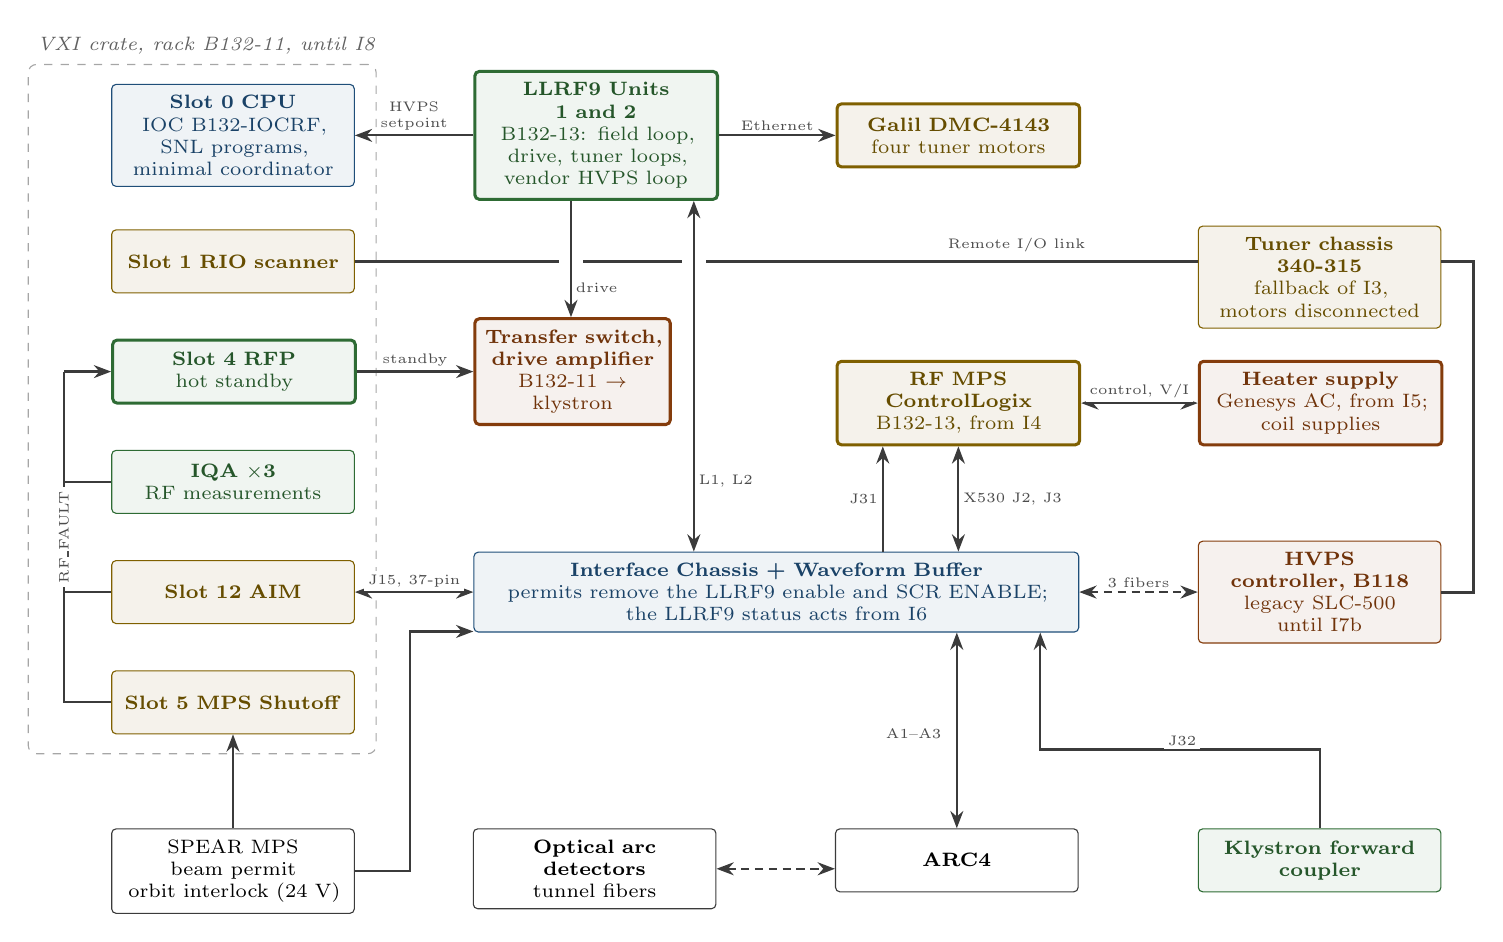
\begin{tikzpicture}[font=\scriptsize, x=1mm, y=1mm,
  every node/.append style={execute at begin node=\hyphenpenalty 10000\relax},
  chg/.style={line width=1.1pt},
  two/.style={{Stealth[length=2.2mm]}-{Stealth[length=2.2mm]},thick,draw=cNeut}]

% ----- VXI crate (column 1), until I8 --------------------------------------
\node[ctrl,text width=28mm,anchor=west] (cpu) at (10,-4)
  {\textbf{Slot 0 CPU}\\ IOC B132-IOCRF,\\ SNL programs,\\ minimal coordinator};
\node[plc,text width=28mm,anchor=west] (scn) at (10,-20)
  {\textbf{Slot 1 RIO scanner}};
\node[rf,chg,text width=28mm,anchor=west] (rfp) at (10,-34)
  {\textbf{Slot 4 RFP}\\ hot standby};
\node[rf,text width=28mm,anchor=west]  (iqa) at (10,-48)
  {\textbf{IQA $\times$3}\\ RF measurements};
\node[plc,text width=28mm,anchor=west] (aim) at (10,-62)
  {\textbf{Slot 12 AIM}};
\node[plc,text width=28mm,anchor=west] (s5)  at (10,-76)
  {\textbf{Slot 5 MPS Shutoff}};
\node[inner sep=0pt,minimum size=0pt] (lane) at (2,-50) {};
\node[grp,fit=(cpu)(scn)(rfp)(iqa)(aim)(s5)(lane)] (crate) {};
\node[lbl,anchor=south west] at (crate.north west) {VXI crate, rack B132-11, until I8};

\draw[thick,draw=cNeut] (s5.west) -- (s5.west -| 4,0) -- (rfp.west -| 4,0);
\draw[thick,draw=cNeut] (aim.west) -- (aim.west -| 4,0);
\draw[thick,draw=cNeut] (iqa.west) -- (iqa.west -| 4,0);
\draw[sig] (rfp.west -| 4,0) -- (rfp.west);
\node[tag,rotate=90] at (4,-55) {RF\_FAULT};

% ----- LLRF9, Galil and the drive --------------------------------------------
\node[rf,chg,text width=28mm,anchor=west] (llrf) at (56,-4)
  {\textbf{LLRF9 Units 1 and 2}\\ B132-13: field loop,\\ drive, tuner loops,\\ vendor HVPS loop};
\node[plc,chg,text width=28mm,anchor=west] (gal) at (102,-4)
  {\textbf{Galil DMC-4143}\\ four tuner motors};
\node[pwr,chg,text width=22mm,anchor=west] (drv) at (56,-34)
  {\textbf{Transfer switch,}\\ \textbf{drive amplifier}\\ B132-11 $\rightarrow$ klystron};
\draw[sig] (llrf.east) -- (gal.west) node[tag,midway,above]{Ethernet};
\draw[sig] (llrf.west) -- (cpu.east) node[tag,midway,above,align=center]{HVPS\\ setpoint};
\draw[sig] (rfp.east) -- (rfp.east -| drv.west) node[tag,midway,above]{standby};

% ----- RF MPS and heater -------------------------------------------------------
\node[plc,chg,text width=28mm,anchor=west] (mps) at (102,-38)
  {\textbf{RF MPS ControlLogix}\\ B132-13, from I4};
\node[pwr,chg,text width=28mm,anchor=west] (htr) at (148,-38)
  {\textbf{Heater supply}\\ Genesys AC, from I5;\\ coil supplies};
\draw[two] (mps.east) -- (htr.west) node[tag,midway,above]{control, V/I};

% ----- Remote I/O link: the PLC-5 node is gone, the tuner and HVPS nodes stay ----
\node[plc,text width=28mm,anchor=west] (tun) at (148,-22)
  {\textbf{Tuner chassis 340-315}\\ fallback of I3,\\ motors disconnected};
\node[pwr,text width=28mm,anchor=west] (hv)  at (148,-62)
  {\textbf{HVPS controller, B118}\\ legacy SLC-500\\ until I7b};
\draw[bus] (scn.east) -- (scn.east -| tun.west);
\draw[bus] (tun.east |- 0,-20) -- (183,-20) |- (hv.east);
\node[tag,anchor=south] at (125,-19.4) {Remote I/O link};
% gaps in the bus where the LLRF9 lines pass over it
\fill[white] (66.9,-21.6) rectangle (69.9,-18.4);
\fill[white] (82.5,-21.6) rectangle (85.5,-18.4);

% ----- the Interface Chassis ---------------------------------------------------
\node[ctrl,text width=74mm,anchor=west] (ic) at (56,-62)
  {\textbf{Interface Chassis + Waveform Buffer}\\
   permits remove the LLRF9 enable and SCR ENABLE;\\
   the LLRF9 status acts from I6};
\draw[sig] (68.4,0 |- llrf.south) -- (68.4,0 |- drv.north) node[tag,pos=0.75,right]{drive};
\draw[two] (84,0 |- llrf.south) -- (84,0 |- ic.north) node[tag,pos=0.8,right]{L1, L2};
\draw[two] (aim.east) -- (ic.west) node[tag,midway,above]{J15, 37-pin};
\draw[two,densely dashed] (ic.east) -- (hv.west) node[tag,midway,above]{3 fibers};
\draw[two] (mps.south) -- (mps.south |- ic.north) node[tag,midway,right]{X530 J2, J3};
\draw[sig] (108,0 |- ic.north) -- (108,0 |- mps.south) node[tag,midway,left]{J31};

% ----- permits, arc detection, forward power ------------------------------------
\node[blk,text width=28mm,anchor=north] (ext) at (s5.south |- 0,-92)
  {SPEAR MPS beam permit\\ orbit interlock (24 V)};
\draw[sig] (ext.north) -- (s5.south);
\draw[sig] (ext.east) -| (48,-67) -- (ic.west |- 0,-67);
\node[blk,text width=28mm,anchor=north] (det) at (71.4,-92)
  {\textbf{Optical arc detectors}\\ tunnel fibers};
\node[blk,text width=28mm,anchor=north] (arc) at (117.4,-92) {\textbf{ARC4}};
\draw[two,densely dashed] (det.east) -- (det.east -| arc.west);
\draw[two] (arc.north) -- (arc.north |- ic.south);
\node[tag,anchor=east] at (116,-80) {A1--A3};
\node[rf,text width=28mm,anchor=north] (kf) at (hv.south |- 0,-92)
  {\textbf{Klystron forward}\\ \textbf{coupler}};
\draw[sig] (kf.north) |- (128,-82) -- (128,0 |- ic.south);
\node[tag,anchor=south] at (146,-82) {J32};
\end{tikzpicture}

\end{fitpicture}
\caption[The station after I6 and I7a.]{The station after I6, drawn with I3 to I5
done; I7a adds no wiring. LLRF9 Unit~1 drives the klystron through the transfer
switch, with the RFP as hot standby, and runs the tuner loops through the Galil, to
which the tuner motors moved at I3. The station permits remove the LLRF9 enable and
SCR ENABLE, and the LLRF9 status acts on SCR ENABLE; RF\_FAULT acts only on the
standby RFP. From I7a the vendor HVPS loop writes the HVPS setpoint through
\mbox{B132-IOCRF} and the Remote I/O link to the legacy SLC-500. The ControlLogix,
off the Remote I/O link, has replaced the PLC-5 (I4) and controls the heater supply
(I5). Heavy outlines: changed since \cref{fig:after-ic}; dashed: fibers.}\label{fig:after-drive}
\end{figure}

\paragraph{Interfaces.}
\begin{itemize}
\item Drive: the drive-amplifier input in B132-11 becomes an interlocked RF transfer
switch with its position read into EPICS, instead of a patch cable.
\item Reference: output RF3 of the VXI CLK module, as in 2021 \R{8}, until the
separate reference distribution of I8.
\item Interlocks: the daisy chain wired at I2 (I2-H2) \R{1}, \R{40}. A unit trips on its
external input or any of its 17 internal sources; Unit~1 then turns off the drive and
opens the absorptive switches in its output chains \R{40}. Since I3 the station
permits remove the LLRF9 enable; with the LLRF9 driving, that now removes the RF. The
LLRF9 status, recorded since I2, now acts on SCR ENABLE (Doc~C D12).
\item EPICS: the vendor station state machine and HVPS loop \R{39}, or the legacy
HVPS loop fed from the LLRF9 (\cref{sec:coordinator}); exactly one loop writes
\fpath{SRF1:HVPS:VOLT:CTRL}.
\end{itemize}

With the LLRF9 driving, RF\_FAULT no longer removes the drive, and every fast RF-off
path has to reach the LLRF9 another way (\cref{tab:protection}).

\begin{longtable}[c]{@{}Q{\cw{0.24}{1.333}}Q{\cw{0.34}{1.333}}Q{\cw{0.42}{1.333}}@{}}
\caption{Fast RF-off paths with the LLRF9 driving.}\label{tab:protection}\\
\toprule
Fault source & Legacy fast action & Required with the LLRF9 driving \\
\midrule
\endfirsthead
\toprule
Fault source & Legacy fast action & Required with the LLRF9 driving \\
\midrule
\endhead
\bottomrule
\endlastfoot
Reflected power, cavity field & IQA amplitude comparators assert RF\_FAULT & The
LLRF9's own interlocks: an overvoltage comparator on each RF input and eight
slow-ADC window comparators \R{40} \\
Arc (ARC4) & --- & The Interface Chassis removes the LLRF9 enable and SCR ENABLE \\
SPEAR MPS beam permit, orbit interlock & Slot~5 asserts RF\_FAULT; from I2 the
Interface Chassis removes SCR ENABLE & The Interface Chassis also removes the LLRF9
enable \\
RF MPS trip & AB summary to the AIM; collector and waveguide-pressure summaries into
the panel's logic & The Interface Chassis removes SCR ENABLE on the AB summary, as
since I2, and the LLRF9 enable, as since I3 \\
HVPS controller trip, including its klystron-arc and transformer-arc triggers & High
voltage removed; STATUS goes dark; the drive stays on until
the state machine turns it off & STATUS also removes the LLRF9 enable \R{3} \\
AIM and the other RF\_FAULT sources in the crate & RF\_FAULT & The state machine acts,
unless an AIM output reaches the Interface Chassis (O3) \\
\end{longtable}

\paragraph{Worklist.} \Cref{tab:wl-i6}. Two spare LLRF9 units exist \R{37}.

\begin{longtable}[c]{@{}Q{\cw{0.10}{1.333}}Q{\cw{0.70}{1.333}}Q{\cw{0.20}{1.333}}@{}}
\caption{Worklist of I6.}\label{tab:wl-i6}\\
\toprule
Item & Work & Depends on \\
\midrule
\endfirsthead
\toprule
Item & Work & Depends on \\
\midrule
\endhead
\bottomrule
\endlastfoot
I6-H1 & The interlocked RF transfer switch at the drive-amplifier input in B132-11,
its position read into EPICS & --- \\
I6-H2 & The LLRF9 interlock daisy chain, wired at I2 (I2-H2), checked with Unit~1
driving: a trip of either unit, or a removed enable, stops the drive & I2-H2 \\
I6-H3 & The SPEAR MPS and orbit permits, wired at I2 and removing the LLRF9 enable
since I3, checked to stop the drive & I2-H6, I3-T6 \\
I6-S1 & SW9: the vendor state machine configured for SPEAR3 (open-loop turn-on, tuning
check, loop close, ramp, turn-off) and commanded by the minimal coordinator in step
with the legacy state machine \R{39} & O5, D11 \\
I6-S2 & SW9: one HVPS loop on the drive power---the vendor loop or the legacy loop fed
from the LLRF9---and an interlock that keeps the other from writing the setpoint
(\cref{sec:coordinator}) & D11 \\
I6-S3 & The vendor links re-pointed from the SRFTEST names to the SRF1 names: drive
power, HVPS minimum and maximum, collector power and the HVPS setpoint \R{39} & O7,
I0-S3 \\
I6-S4 & SW9: the RFP-specific SNL functions disabled; the fault response (HVPS
ramp-down and SCR disable, Interface Chassis reset) & O5 \\
I6-T1 & Bench: the LLRF9 interlock chain with the Interface Chassis, each internal
source and the external input; the transfer-switch interlock & I6-H1, I6-H2 \\
I6-T2 & With the LLRF9 driving: the transfer at low power, following the switching,
interlock and turn-on procedure of the 2021 tests (O7); every path of
\cref{tab:protection}; the hand-over of the HVPS loop, with only one loop writing
the setpoint; an Interface Chassis reset while the LLRF9 drives (Doc~C RS-4) &
I6-S1 to I6-S4 \\
I6-T3 & Stability, ripple rejection and synchrotron-line damping against acceptance
criteria agreed before the window. In 2021 the LLRF9 rejected the
\qty{\pm 360}{\hertz} and \qty{\pm 720}{\hertz} ripple by
\qtyrange{16}{21}{\decibel} against \qtyrange{24}{27}{\decibel} for the legacy
system, with the synchrotron line at \qty{9657}{\hertz} and a quality factor of 16.7
against \qty{8932}{\hertz} and 11.1 \R{9} & I6-T2 \\
\end{longtable}

\paragraph{Entry criteria.} I2, with the ARC4 trip, the Waveform Buffer comparators
and the machine permits acting after the record of I2-T4; O5 and O6 closed; I6-S1 to
I6-S4; I6-H1; the
acceptance criteria; a record of the LLRF9 interlocks, kept from I2 on.

\paragraph{Fallback.} The transfer switch back to the RFP and the legacy SNL
configuration restored.

% ---------------------------------------------------------------------------
\subsection{I7: HVPS Control by the LLRF9 and New HVPS Controllers}\label{sec:i-hvps}

\paragraph{Scope.} I7 changes the HVPS in three steps, each of which changes one thing
and has a tested fallback:
\begin{description}
\item[I7a] the LLRF9 and the coordinator take over HVPS control on the legacy
controllers, with no hardware change (\cref{sec:i-hvps-a});
\item[I7b] a new Hoffman box and PPS Interface Box replace the legacy box of the
off-duty unit, with the other unit, still legacy, as the fallback
(\cref{sec:i-hvps-b});
\item[I7c] the second unit is converted in the same way once the first has run for
some months without a fault caused by the controller (\cref{sec:i-hvps-c}).
\end{description}
Both units must be converted before I8 removes the RIO link, the only path from the
IOC to a legacy SLC-500. One unit is energized at a time, and the units exchange roles
in scheduled downs, typically in April and August \R{1}. The switch-over takes hours,
with both supplies locked out, and breaks the PPS chain \R{31}, so a fallback from one
unit to the other is a planned job in a down.

\subsubsection{I7a: HVPS Control by the LLRF9 on the Legacy Controllers}\label{sec:i-hvps-a}

\paragraph{Scope.} The vendor HVPS loop on the LLRF9 drive power becomes the one loop
that writes \fpath{SRF1:HVPS:VOLT:CTRL}, sequenced by the vendor state machine and the
coordinator's fault response (SW9), through today's path: \mbox{B132-IOCRF}, the RIO
scanner in the VXI crate, the 1747-DCM and the SLC-500 of the unit in service, whose
program sets the regulator reference within its own ramp and limits. If I6 kept the
legacy HVPS loop (D11), the hand-over to the vendor loop is made here. Nothing changes
in B118 or B514. I7a is the hold point before the new controller: the station runs
with the new control on the legacy controllers long enough to give I7b its baseline
and a configuration to fall back to.

\paragraph{Interfaces.}
\begin{itemize}
\item EPICS: the HVPS records under their current names
(Appendix~\ref*{app:epics}); the vendor loop's minimum and maximum are the legacy
limits, and its inputs are re-pointed to the SRF1 names (I6-S3) \R{39}.
\item The HVPS-on request still reaches the Interface Chassis from the legacy state
machine through the AIM until I8; the fibers and the monitor outputs are as today.
\item The two legacy units and the switch-over between them are unchanged \R{31}.
\end{itemize}

\paragraph{Worklist.} \Cref{tab:wl-i7a}.

\begin{longtable}[c]{@{}Q{\cw{0.10}{1.333}}Q{\cw{0.70}{1.333}}Q{\cw{0.20}{1.333}}@{}}
\caption{Worklist of I7a.}\label{tab:wl-i7a}\\
\toprule
Item & Work & Depends on \\
\midrule
\endfirsthead
\toprule
Item & Work & Depends on \\
\midrule
\endhead
\bottomrule
\endlastfoot
I7a-S1 & SW9: the vendor HVPS loop as the only writer of \fpath{SRF1:HVPS:VOLT:CTRL}
on the legacy controllers, within the legacy minimum and maximum, sequenced by the
vendor state machine and the coordinator's fault response; the hand-over from the
legacy loop if I6 kept it (D11) & I6-S2 \\
I7a-T1 & With beam: the vendor loop regulating through the SLC-500, its steps against
the SLC-500's ramp and limits, and the minimum it sets at an LLRF9 interlock trip; the
turn-on, turn-off and fault ramps; regulation, ripple and trips recorded as the
baseline of I7b & I7a-S1 \\
I7a-T2 & A switch-over between the two legacy units with the new control, timed, as a
rehearsal of the fallback of I7b \R{31} & I7a-T1 \\
\end{longtable}

\paragraph{Entry criteria.} I6 in operation; I7a-S1 tested on the test IOC.

\paragraph{Fallback.} The configuration of I6, with the legacy HVPS loop if I6 used
it, restored by the selection of SW9 (I6-S2).

\subsubsection{I7b: First New Hoffman Box}\label{sec:i-hvps-b}

\paragraph{Scope.} The HVPS controller of the off-duty unit is replaced as a whole: a
new Hoffman box, built around the CompactLogix, the FCOG1200 firing boards and the
redesigned regulator, retires that unit's existing box in B118 with its SLC-500,
firing and regulator boards, trigger interconnect boards, power supplies and local
control panel. In the same down and under one PPS certification the PPS Interface Box
takes that unit's PPS chains out of the PLC. The other unit keeps its legacy box and
PPS wiring, in the configuration of I7a, as the fallback. The CompactLogix is online
with EPICS communication and its ladder program is still being completed; the
FCOG1200 boards are ordered and the regulator is being redesigned \R{1}.

\paragraph{Interfaces.}
\begin{itemize}
\item Field cables: the existing cables to the HVPS power section, the contactor
controller and the grounding tank land on the new box unchanged \R{1}, among them the
klystron-arc coax from the Pearson current transformer and the transformer-arc
trigger, which fire the crowbar in hardware \R{5}, \R{25}.
\item HVPS fibers: the three fibers from the Interface Chassis with unchanged light
conventions; the new box keeps the trigger inhibit of \cref{sec:hwchain}, which leaves
B$^+$ and B$^-$ firing so that the filter inductors discharge \R{4}, \R{5}. Its
STATUS goes dark when its processor stops, as with the SLC-500, because the HVPS
controller sends no heartbeat (Doc~C IC-4) \R{45}.
\item The HVPS voltage and current monitor outputs keep their scaling, because the
Interface Chassis buffers them for the collector power and the Waveform Buffer. The
pick-offs of the transformer current and the SCR firing signal for the Waveform
Buffer (Doc~C O8) are made on both kinds of box.
\item EPICS: all HVPS control stays in EPICS, with no Python layer, under the current
PV names in \mbox{B132-IOCRF}: eleven records of the HVPS node plus 32 status bits
(Appendix~\ref*{app:epics}) \R{12}. While one unit is legacy and the other new, the IOC
serves either through two database variants or a selector. The switch-over procedure
moves six terminal blocks, the three fibers and the klystron-arc BNC in a switchbox
in B118, the bus bars of the cable switch tank and the fan breakers in B514 \R{31};
with one legacy and one new box, every line on those blocks has to be listed and every
plug has to fit both boxes.\openitem{O9}
\item RIO: the HVPS node stays on the RIO link while a legacy unit remains, until I7c.
\item PPS: today PPS~1 enters an SLC-500 input and the supply of the output that drives
contactor K4, and PPS~2 enters another input while rung 0016 drives the Ross
grounding-switch coil from a PLC output; chain~2 has no hardware protection against a
PLC output stuck on \R{25}. The PPS box drives K4 and the Ross coil directly, the
Ross coil from PPS~2 alone where the legacy ladder needs both chains \R{1}, \R{2}; this
belongs in the PPS review. Two units need one box each, or a cable moved at the
switch-over, which already breaks the PPS chain \R{31}. Both configurations, the new
box with its PPS box and the legacy box with its PPS wiring, are certified together,
and the PPS chain is checked after each switch-over.
\item The local control panel (touch panel, PERMIT key switch, EMERGENCY OFF button
with two contacts) is reproduced in the new box; the EMERGENCY OFF test of Doc~L (O11)
is part of the commissioning.
\end{itemize}

\paragraph{Worklist.} \Cref{tab:wl-i7b}.

\begin{longtable}[c]{@{}Q{\cw{0.10}{1.333}}Q{\cw{0.70}{1.333}}Q{\cw{0.20}{1.333}}@{}}
\caption{Worklist of I7b.}\label{tab:wl-i7b}\\
\toprule
Item & Work & Depends on \\
\midrule
\endfirsthead
\toprule
Item & Work & Depends on \\
\midrule
\endhead
\bottomrule
\endlastfoot
I7b-H1 & The new Hoffman box for the first unit: CompactLogix, FCOG1200 firing boards,
redesigned regulator, the trigger inhibit of \cref{sec:hwchain}, and the local control
panel with touch panel, PERMIT key switch and two-contact EMERGENCY OFF button & --- \\
I7b-H2 & The PPS Interface Box (B.~Morris): a Bud enclosure with four relays, status
LEDs and one PPS-lockable connector, two permit and two readback channels, the
standard design of the 6575 modulator and gallery systems \R{1}; one per unit, or a
cable moved at the switch-over & A14 \\
I7b-H3 & The field cables landed on the new box unchanged, including the klystron-arc
coax and the transformer-arc trigger; the three fibers; the voltage and current
monitor outputs with unchanged scaling; switchbox plugs that fit both boxes & O9 \\
I7b-H4 & The Waveform Buffer's transformer-current and SCR-firing pick-offs on the new
box, as on the legacy one (Doc~C O8) & I2-H4 \\
I7b-S1 & The CompactLogix program completed and reviewed against the SLC-500
program, with the legacy data image (D5) & D5 \\
I7b-S2 & SW6: the HVPS IOC behind the current names, and the selector or database
variants while one unit is legacy and the other new; SW1 for the legacy database
change & SW1 \\
I7b-T1 & On Test Stand~18 in B44, upgraded for the new controller: the new box running
the test-stand HVPS \R{1}; its processor stopped, with STATUS going dark (Doc~C IC-4)
& I7b-H1, I7b-S1 \\
I7b-T2 & At SPEAR3, the new box against the baseline of I7a: regulation and ripple;
every HVPS interlock and crowbar source, including the klystron-arc and
transformer-arc triggers; the fiber trio with the Interface Chassis; the vendor HVPS
loop writing the same setpoint name & I7b-T1, I7a-T1 \\
I7b-T3 & PPS certification of both configurations; the EMERGENCY OFF test of Doc~L
(O11); the PPS chain checked after the switch-over & A14 \\
I7b-T4 & A run with beam on the new box against acceptance criteria agreed before the
window, ending in the decision to keep it or to fall back and in the criteria for I7c
& I7b-T2 \\
\end{longtable}

\paragraph{Entry criteria.} The PPS steps of A14, ending in ADSO approval of the final
design and documentation of the PPS box; the Radiation Safety Work Control Form;
I7b-H1 complete, bench-tested and run on Test Stand~18 (I7b-T1); I7b-S1 and I7b-S2;
O9 closed; the baseline of I7a-T1 and the rehearsal of I7a-T2.

\paragraph{Fallback.} Switch-over to the other unit, with its legacy Hoffman box and
PPS wiring, in the configuration of I7a: a planned job of some hours in a down,
rehearsed in I7a-T2.

\subsubsection{I7c: Second New Hoffman Box}\label{sec:i-hvps-c}

\paragraph{Scope.} Once the first new box has run for some months without a fault
caused by the controller, by the criteria of I7b-T4, the second unit's box is replaced
in the same way while that unit is off duty, with its own PPS Interface Box. No legacy
HVPS controller then remains: the HVPS node leaves the RIO link, and the IOC drops the
legacy database variant.

\paragraph{Worklist.} \Cref{tab:wl-i7c}.

\begin{longtable}[c]{@{}Q{\cw{0.10}{1.333}}Q{\cw{0.70}{1.333}}Q{\cw{0.20}{1.333}}@{}}
\caption{Worklist of I7c.}\label{tab:wl-i7c}\\
\toprule
Item & Work & Depends on \\
\midrule
\endfirsthead
\toprule
Item & Work & Depends on \\
\midrule
\endhead
\bottomrule
\endlastfoot
I7c-H1 & The second new Hoffman box and its PPS Interface Box, as in I7b-H1 to I7b-H4
& I7b-T4 \\
I7c-H2 & The HVPS node removed from the RIO link and the chain re-terminated &
I7c-T2 \\
I7c-S1 & SW6: the selector or the legacy database variant removed & I7c-T2 \\
I7c-T1 & The second box run on Test Stand~18, as in I7b-T1 & I7c-H1 \\
I7c-T2 & At SPEAR3, the tests of I7b-T2 and I7b-T3, against the first new unit &
I7c-T1 \\
\end{longtable}

\paragraph{Entry criteria.} The run record of I7b against its criteria (I7b-T4);
I7c-T1; the PPS approval of the second PPS box.

\paragraph{Fallback.} The first new unit. The second unit's legacy box is kept until
I7c-T2 has passed.

% ---------------------------------------------------------------------------
\subsection{I8: Legacy Retirement}\label{sec:i-retire}

\paragraph{Scope.} The VXI crate is removed with its CPU, RIO scanner, CLK module,
RFP, IQAs, AIM and Slot~5, together with the tuner chassis, the RIO link and the spare
Fast Interlock Chassis and panel. The IOC \mbox{B132-IOCRF} moves to new hardware with
the full coordinator (\cref{fig:after-retire}).

% [H]: a float here is held back behind the I8 worklist into the next section
\begin{figure}[H]
\centering
\begin{fitpicture}
% !TeX root = ../M_integration_migration_plan.tex
% The station after I8: no VXI crate, no Remote I/O link, no tuner chassis. Same grid
% as fig-after-drive; the controls network takes the row of the Remote I/O link.
% Heavy outlines mark what changed since fig-after-drive. The LLRF9 lines and the
% reference pass over the network.
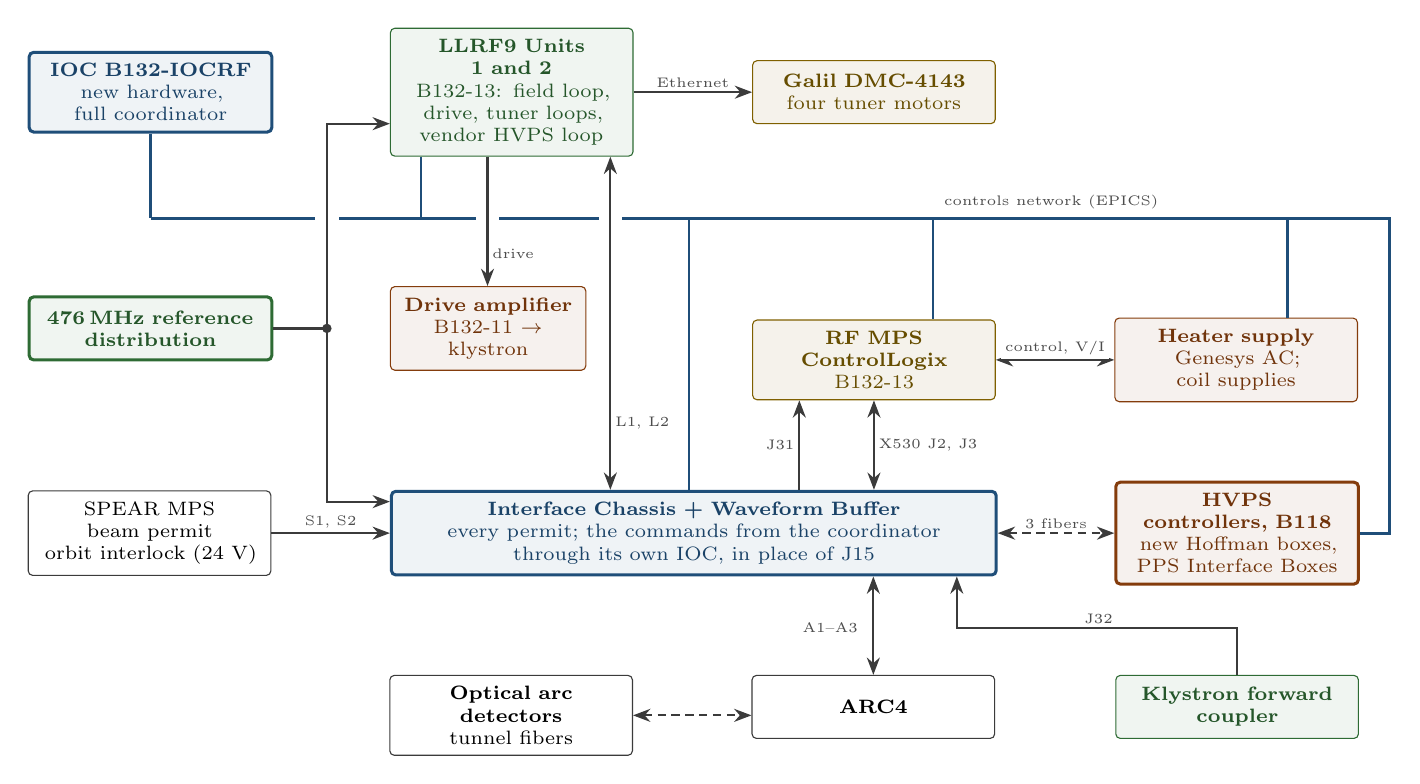
\begin{tikzpicture}[font=\scriptsize, x=1mm, y=1mm,
  every node/.append style={execute at begin node=\hyphenpenalty 10000\relax},
  chg/.style={line width=1.1pt},
  two/.style={{Stealth[length=2.2mm]}-{Stealth[length=2.2mm]},thick,draw=cNeut},
  tap/.style={draw=cCtrl,thick}]

% ----- coordinator, reference and machine permits (column 1) -------------------
\node[ctrl,chg,text width=28mm,anchor=west] (cpu) at (10,-4)
  {\textbf{IOC B132-IOCRF}\\ new hardware,\\ full coordinator};
\node[rf,chg,text width=28mm,anchor=west] (ref) at (10,-34)
  {\textbf{476\,MHz reference}\\ \textbf{distribution}};
\node[blk,text width=28mm,anchor=west] (ext) at (10,-60)
  {SPEAR MPS beam permit\\ orbit interlock (24 V)};

% ----- LLRF9, Galil and the drive --------------------------------------------
\node[rf,text width=28mm,anchor=west] (llrf) at (56,-4)
  {\textbf{LLRF9 Units 1 and 2}\\ B132-13: field loop,\\ drive, tuner loops,\\ vendor HVPS loop};
\node[plc,text width=28mm,anchor=west] (gal) at (102,-4)
  {\textbf{Galil DMC-4143}\\ four tuner motors};
\node[pwr,text width=22mm,anchor=west] (drv) at (56,-34)
  {\textbf{Drive amplifier}\\ B132-11 $\rightarrow$ klystron};
\draw[sig] (llrf.east) -- (gal.west) node[tag,midway,above]{Ethernet};

% ----- RF MPS, heater and HVPS -----------------------------------------------------
\node[plc,text width=28mm,anchor=west] (mps) at (102,-38)
  {\textbf{RF MPS ControlLogix}\\ B132-13};
\node[pwr,text width=28mm,anchor=west] (htr) at (148,-38)
  {\textbf{Heater supply}\\ Genesys AC;\\ coil supplies};
\draw[two] (mps.east) -- (htr.west) node[tag,midway,above]{control, V/I};
\node[pwr,chg,text width=28mm,anchor=west] (hv)  at (148,-60)
  {\textbf{HVPS controllers, B118}\\ new Hoffman boxes,\\ PPS Interface Boxes};

% ----- the Interface Chassis ---------------------------------------------------
\node[ctrl,chg,text width=74mm,anchor=west] (ic) at (56,-60)
  {\textbf{Interface Chassis + Waveform Buffer}\\
   every permit; the commands from the coordinator\\
   through its own IOC, in place of J15};

% ----- controls network, in the row of the old Remote I/O link -------------------
\draw[bus,draw=cCtrl] (cpu.south |- 0,-20) -- (183,-20) |- (hv.east);
\node[tag,anchor=south] at (140,-19.4) {controls network (EPICS)};
\draw[tap] (cpu.south) -- (cpu.south |- 0,-20);
\draw[tap] (60,0 |- llrf.south) -- (60,-20);
\draw[tap] (94,-20) -- (94,0 |- ic.north);
\draw[tap] (125,-20) -- (125,0 |- mps.north);
\draw[tap] (170,-20) -- (170,0 |- htr.north);
% gaps in the network where the reference and the LLRF9 lines pass over it
\fill[white] (46.5,-21.6) rectangle (49.5,-18.4);
\fill[white] (66.9,-21.6) rectangle (69.9,-18.4);
\fill[white] (82.5,-21.6) rectangle (85.5,-18.4);

% ----- RF, interlock and reference lines ---------------------------------------
\draw[sig] (68.4,0 |- llrf.south) -- (68.4,0 |- drv.north) node[tag,pos=0.75,right]{drive};
\draw[two] (84,0 |- llrf.south) -- (84,0 |- ic.north) node[tag,pos=0.8,right]{L1, L2};
\draw[thick,draw=cNeut] (ref.east) -- (48,-34);
\draw[sig] (48,-34) |- (llrf.west |- 0,-8);
\draw[sig] (48,-34) |- (ic.west |- 0,-56);
\fill[cNeut] (48,-34) circle (0.6);
\draw[sig] (ext.east) -- (ic.west) node[tag,midway,above]{S1, S2};
\draw[two,densely dashed] (ic.east) -- (hv.west) node[tag,midway,above]{3 fibers};
\draw[two] (mps.south) -- (mps.south |- ic.north) node[tag,midway,right]{X530 J2, J3};
\draw[sig] (108,0 |- ic.north) -- (108,0 |- mps.south) node[tag,midway,left]{J31};

% ----- arc detection and forward power, as since I2 ------------------------------
\node[blk,text width=28mm,anchor=north] (det) at (71.4,-78)
  {\textbf{Optical arc detectors}\\ tunnel fibers};
\node[blk,text width=28mm,anchor=north] (arc) at (117.4,-78) {\textbf{ARC4}};
\draw[two,densely dashed] (det.east) -- (det.east -| arc.west);
\draw[two] (arc.north) -- (arc.north |- ic.south);
\node[tag,anchor=east] at (116,-72) {A1--A3};
\node[rf,text width=28mm,anchor=north] (kf) at (hv.south |- 0,-78)
  {\textbf{Klystron forward}\\ \textbf{coupler}};
\draw[sig] (kf.north) |- (128,-72) -- (128,0 |- ic.south);
\node[tag,anchor=south] at (146,-72) {J32};
\end{tikzpicture}

\end{fitpicture}
\caption[The station after I8.]{The station after I8: the VXI crate, the Remote I/O
link and the tuner chassis are gone. \mbox{B132-IOCRF} runs the full coordinator on new
hardware and reaches every subsystem over the controls network; the Interface Chassis
alone takes the machine permits and gets its commands through its own IOC. Heavy
outlines: changed since \cref{fig:after-drive}; dashed: fibers.}\label{fig:after-retire}
\end{figure}

\paragraph{What changes.}
\begin{itemize}
\item The AIM's commands to the Interface Chassis---station online, filament and
focus, HVPS on and filament-timeout requests and the fault reset---come
from the coordinator through the Interface Chassis IOC instead of J15.
\item The SPEAR MPS and orbit permits reach only the Interface Chassis.
\item The LLRF9 reference comes from a separate \qty{476}{\mega\hertz} distribution.
\item The transfer switch stays on the LLRF9, and the RFP is gone.
\item Every legacy function of \cref{tab:orphans} has its new home.
\item Links to legacy names move with the names: the vendor HVPS loop reads its drive
power from an IQA today, so it is re-pointed to the klystron-drive channel of LLRF9
Unit~2 \R{1}, \R{39}.
\end{itemize}

\paragraph{Worklist.} \Cref{tab:wl-i8}.

\begin{longtable}[c]{@{}Q{\cw{0.10}{1.333}}Q{\cw{0.70}{1.333}}Q{\cw{0.20}{1.333}}@{}}
\caption{Worklist of I8.}\label{tab:wl-i8}\\
\toprule
Item & Work & Depends on \\
\midrule
\endfirsthead
\toprule
Item & Work & Depends on \\
\midrule
\endhead
\bottomrule
\endlastfoot
I8-H1 & The separate \qty{476}{\mega\hertz} reference distribution for the LLRF9 and the
Waveform Buffer & --- \\
I8-H2 & New hardware for \mbox{B132-IOCRF} & --- \\
I8-H3 & No new drive-power measurement for the HVPS loop: LLRF9 Unit~2 measures the
klystron drive from I1 \R{1}, compared with the IQA in I1-T2 & I1-H3 \\
I8-H4 & Removal of the VXI crate, the tuner chassis, the RIO link and the spare Fast
Interlock Chassis and panel; as-built drawings of the new station \R{37} & I8-T1 \\
I8-S1 & SW10: the full coordinator on the new hardware (\cref{sec:coordinator}) & D9
\\
I8-S2 & SW7: the command path from the Interface Chassis IOC in place of J15, among
them the station-online command, the only online/offline control from I2 \R{45} & I2-H1
\\
I8-S3 & Every Channel Access link to a retired legacy name re-pointed, among them the
LLRF9's drive-power and collector-power links; legacy names that are not kept retired;
screens, alarm tree and archiver moved & D3 \\
I8-T1 & SW10 tested on the new hardware with every subsystem in its final form & I1 to
I7 \\
I8-T2 & An end-to-end interlock test with fault injection on every layer & I8-T1 \\
I8-T3 & Full-power commissioning; operator training & I8-T2 \\
\end{longtable}

\paragraph{Entry criteria.} I1 to I7c complete, with both HVPS units on new boxes; a
full run period of I6 without a fallback to the RFP; SW10 tested on the new hardware;
the reference distribution; the Interface Chassis in hub mode and the RF MPS in
upgrade mode; a home for every legacy function.

\paragraph{Fallback.} None practical once the hardware is removed, hence the run
period required at entry.

% ===========================================================================
\section{Legacy Functions and Their New Homes}\label{sec:orphans}

Doc~0 assigns the legacy functions of \cref{tab:orphans}, which have no one-to-one
successor, to their new homes \R{1}. With the panel and the Fast Interlock Chassis gone
at I2, several pass through the Interface Chassis first.

\begin{longtable}[c]{@{}Q{\cw{0.05}{1.6}}Q{\cw{0.22}{1.6}}Q{\cw{0.28}{1.6}}Q{\cw{0.30}{1.6}}Q{\cw{0.15}{1.6}}@{}}
\caption{Legacy functions and their new homes.}\label{tab:orphans}\\
\toprule
\# & Function & Legacy implementation & New home & Moves at \\
\midrule
\endfirsthead
\toprule
\# & Function & Legacy implementation & New home & Moves at \\
\midrule
\endhead
\bottomrule
\endlastfoot
1 & Beam abort to the SPEAR MPS & AIM force and reset by the state
machine; the panel's logic; BNC J6, not cabled at SPEAR3 \R{17}, \R{26} & None: the
SPEAR MPS takes no status from the RF in hardware \R{3}, \R{45} & --- \\
2 & Main focus and bucking-coil supply control and interlocks & PLC-5 through the panel
\R{7} & Interface Chassis passes the lines; later RF MPS outputs & I2; I4 \\
3 & Filament request and timer bypass & AIM, Fast Interlock Chassis, panel and PLC-5
\R{6} & Interface Chassis passes the requests; later RF MPS and heater IOC & I2; I8 \\
4 & HV-detected and RF-detected lamps; online/offline and local/remote key switches &
Lamps driven by the PLC-5; keys into PLC-5 inputs \R{7} & Lamp states reported to EPICS
by the PLC-5, later the RF MPS; online/offline from EPICS, with the online-mode line
held on by the Interface Chassis; no local/remote key \R{45} & I2 \\
5 & Buffered HVPS voltage and current for the collector power & Panel buffers \R{7} &
Interface Chassis buffers; later HVPS controller to RF MPS & I2; I7 \\
6 & HV turn-on gate & AIM ``HVPS on'' request into the panel's logic & Interface
Chassis logic; the request from the coordinator after the AIM is gone & I2; I8 \\
7 & Automatic reset after a trip, with its retry count and forced-fault inhibit & State
machine; AIM forced-fault latch, set by operator command \R{17} & Coordinator & I8 \\
8 & Reference power, crate and RIO health monitors & SNL and VXI records & Reference
distribution monitor; IOC health records & I8 \\
9 & Fault capture and MATLAB fault tools & AIM, IQA and RFP history buffers; MATLAB
tools & LLRF9 and Waveform Buffer post-mortem; ported tools & I6; I8 \\
10 & Readbacks for other subsystems & PLC-5 channels (\cref{sec:plc5data}) & RF MPS,
with the same names & I4 \\
11 & \qty{476}{\mega\hertz} reference distribution & VXI CLK module & Separate
reference distribution chassis & I8 \\
12 & Drive power for the HVPS loop & IQA measurement of the klystron drive \R{16}, also
read by the vendor HVPS loop \R{39} & The klystron-drive channel of LLRF9 Unit~2, from
I1 \R{1} & I8 \\
\end{longtable}

% ===========================================================================
\section{Software Plan}\label{sec:software}

\subsection{Coordinator and Principles}\label{sec:principles}

The coordinator is the IOC \mbox{B132-IOCRF}: a minimal release (SW9) on the VXI CPU
for I6, which needs the legacy build environment (O5), and a full release (SW10) on new
hardware for I8, each with one adapter per subsystem that talks to either the legacy or
the new hardware, so that the order of I4 to I7 can change (\cref{sec:coordinator}).
All HVPS functions stay in EPICS, with no Python layer. Principles:
\begin{enumerate}
\item \textbf{Minimum software per integration.} The legacy SNL programs stay in charge
until I6, so every integration except I6 and I8 needs only its subsystem IOC and, at most, a
legacy database change.
\item \textbf{Generate rather than write.} With a legacy data image in the new PLCs
(\cref{sec:image}), the legacy substitution files generate most of the RF MPS and HVPS
databases; alarm limits come from the IOC's saved settings, because the archived files
differ from the live values (\cref{sec:i-heater}).
\item \textbf{Standard modules and vendor software first}: the LLRF9's own IOC with its
tuner loops, Galil driver, station state machine and HVPS loop \R{39}, a standard
driver for the Genesys AC, and the EtherNet/IP driver for the ControlLogix and
CompactLogix.
\end{enumerate}

\subsection{Work Packages}\label{sec:wp}

Every work package is led by the controls group, with technical support from the lead
of the subsystem it serves, named in \cref{tab:wp}.

\begin{longtable}[c]{@{}Q{\cw{0.08}{1.6}}Q{\cw{0.46}{1.6}}Q{\cw{0.12}{1.6}}Q{\cw{0.13}{1.6}}Q{\cw{0.21}{1.6}}@{}}
\caption{Software work packages, led by the controls group.}\label{tab:wp}\\
\toprule
WP & Content & Needed for & Relative size & Technical support \\
\midrule
\endfirsthead
\toprule
WP & Content & Needed for & Relative size & Technical support \\
\midrule
\endhead
\bottomrule
\endlastfoot
SW0 & PV naming policy, legacy compatibility rules, one interface control document per
integration & All & Small & Project lead \\
SW1 & Owner for the legacy IOC; test IOC; procedure to edit and reload
\fpath{srf1.db}; check of the SNL build & I3, I4, I6, I7 & Small to medium & J.~Sebek \\
SW2 & LLRF9 tuner loops driving the Galil: the vendor driver configuration extended to
four axes, limits, home move and bench test; legacy tuner loops off and their alarms
adjusted; optionally the vendor stepper interface & I3 & Small & M.~Dunning \\
SW3 & Heater IOC (Genesys AC over Ethernet) & I5 & Small & B.~Morris \\
SW4 & ARC4 permit and fired detector, read out from the Interface Chassis IOC to the
screens, alarms and legacy links that read the AIM's arc records today & I2 & Small &
D.~Zhang \\
SW5 & RF MPS IOC generated from the legacy substitution files, the saved settings and
the legacy data image; legacy records re-pointed & I4 & Medium & M.~Larrus \\
SW6 & HVPS IOC behind the current HVPS names in \mbox{B132-IOCRF}; selector in the
legacy database for the legacy or new HVPS unit & I7b & Small & M.~Larrus \\
SW7 & Interface Chassis and Waveform Buffer IOC: states, first fault,
waveforms; archiving, alarms and post-mortem capture; the LLRF9 reset after each
chassis reset and the freeze on a legacy RF fault; later the command path that
replaces J15 & I2, I8 & Medium & J.~Sebek,
D.~Zhang, D.~Scott \\
SW8 & LLRF9 configuration, cross-calibration, screens, alarms and archiving; the
monitor-only safeguards of I1 and the review of the vendor links to legacy PVs & I1, I6
& Medium & J.~Sebek, M.~Dunning, D.~Scott \\
SW9 & Minimal coordinator in \mbox{B132-IOCRF} on the VXI CPU, commanding the vendor
state machine and one HVPS loop (\cref{sec:coordinator}) & I6, I7a & Medium & J.~Sebek \\
SW10 & Full coordinator in \mbox{B132-IOCRF} on its new hardware, operator screens,
post-mortem tools, ported MATLAB tools & I8 & Large & J.~Sebek \\
\end{longtable}

\subsection{Adapting the Legacy IOC}\label{sec:legacyioc}

When a legacy PLC is replaced, the legacy records that read it keep their names, alarm
limits and summaries, and their data source changes from the RIO link to Channel
Access links to the new IOC; the alarm tree and screens stay unchanged, and the new IOC
keeps neutral names. Recreating the records in the new IOC under the legacy names would
instead need every alarm limit and summary link reproduced exactly. Each legacy
database change follows one procedure: edit; test on the test IOC; apply in a down with
the previous \fpath{srf1.db} and \fpath{config.ab} kept; verify the alarm tree and the
SNL behavior; record the configuration. A named owner for the legacy IOC and a test IOC
are prerequisites for I3, I4, I6 and I7.

\subsection{Legacy Data Image in the New PLCs}\label{sec:image}

The PLC-5 and the SLC-500 exchange their data with EPICS through the RIO images of
their DCMs, and the legacy records address these images by link, adapter, card and
signal \R{12}, \R{32}. If each new PLC program keeps tag arrays with exactly this
layout, maintained by the ladder logic, the legacy records can be re-pointed one for
one, the new IOC databases can be generated from the legacy substitution files, and
old and new values can be compared word by word during commissioning. The cost is a
small amount of ladder logic; the image is retired with the VXI crate.

For the PLC-5 the program gives the layout \R{38}: eight pages of 64 words, each with
its page number in word~3. Pages 0 and 1 hold the alarm limits of the 112
thermocouples; pages 2 and 3 their readings, with five temperature rises of the
klystron (body, collector and window air) in place of five of its readings; page 4 the
32 raw analog inputs, the first four analog trip limits, the remaining warm-up time
and the collector power with its limit; page 5 the other 60 analog trip limits; page 6
the fault latches, their copy frozen at the last global trip, the module communication
bits and the summaries; page 7 only its number.

\subsection{PV Naming Policy}\label{sec:naming}

Two IOCs serving one name give undefined Channel Access behavior. While a legacy record
exists, its name belongs to \mbox{B132-IOCRF}; the HVPS keeps its current names, such
as \fpath{SRF1:HVPS:VOLT:CTRL} and \fpath{SRF1:HVPS:VOLT:RBCK} \R{12}; other new IOCs
use prefixes that cannot collide with legacy names, such as \fpath{SRF1:MPS:} and
\fpath{SRF1:WFBUF:} in Doc~0 \R{1}. Exceptions are deliberate and recorded, and legacy
names that are not kept are retired with the VXI crate.

\subsection{Coordinator Scope}\label{sec:coordinator}

\paragraph{Minimal release (SW9), for I6.}
\begin{itemize}
\item LLRF9 turn-on and turn-off: the vendor station state machine \R{39}, which
resets the interlocks with a set number of retries, turns on open loop, waits until
the tuning errors are in range, closes the field loop, ramps to the operating point and
ramps down, configured for SPEAR3 and commanded in step with the legacy state machine.
\item One HVPS supervisory loop on the LLRF9 drive power, chosen by D11 from the
options below.
\item Fault response: HVPS ramp-down and SCR disable, and the Interface Chassis reset.
The automatic reset, with its retry count and forced-fault inhibit, stays in the
legacy SNL.
\item Adapters for the subsystems that are still legacy.
\end{itemize}

\paragraph{HVPS loop options for I6.} Exactly one loop writes
\fpath{SRF1:HVPS:VOLT:CTRL}; the others are held open, and the hand-over is tested
(I6-T2).
\begin{enumerate}
\item \textbf{The vendor loop} \R{39}. Every \qty{0.5}{\second} it compares the
klystron drive power with a setpoint of \qty{28}{\watt}, or \qty{29}{\watt} above a
klystron forward power of \qty{600}{\kilo\watt}, and outside a deadband of
\qty{0.1}{\watt} lowers the HVPS voltage by \qty{0.05}{\kilo\volt} per watt of
shortfall, raising it for an excess, at most \qty{0.5}{\kilo\volt} per step, between
the legacy minimum and maximum. Above a collector power of \qty{1000}{\kilo\watt} from
the PLC it only lowers the voltage; when the LLRF9 interlock trips it sets the minimum
once. It runs only with its mode set to closed and the field loop closed, and it
ships open. Its inputs are the IQA drive power and legacy records, under SRFTEST
names, and its output is a record inside the LLRF9 IOC, so all are re-pointed
(I6-S3). It has no states, status codes or tolerance checks of the legacy kind.
\item \textbf{The legacy loop, database only.} J.~Sebek proposes keeping the legacy
HVPS loop while the LLRF9 drives. The loop regulates on database records, such as the
HVPS step \fpath{SRF1:KLYSDRIVFRWD:HVPS:DELTA} computed from the drive power and its
setpoint, and checks the RFP's direct-loop flag and severity,
\fpath{SRF1:STN:RFP:MODU.DLE} and \fpath{SRF1:STN:RFP:MODU.SEVR} \R{16}. Fed from the
LLRF9, or held in their operating state while the RFP stands by, these let the loop
keep regulating with no SNL change. The flag also acts on the RFP and the DAC loop, so
the option is proven on the test IOC first.
\item \textbf{The legacy loop, changed in SNL} so that it no longer depends on the RFP,
keeping its states, status codes and tolerance checks; this needs the SNL build (O5).
\end{enumerate}
With option 1 or 2, I6 needs the SNL build only for other SNL changes, and SW9 shrinks
to commanding the vendor state machine and the fault response. All three read the
klystron drive power from an IQA, which goes at I8; LLRF9 Unit~2 measures it from I1
and takes its place (\cref{tab:orphans}, row 12).

\paragraph{Full release (SW10), for I8.} On the new hardware of \mbox{B132-IOCRF}:
station state machine, the commands to the Interface Chassis that the AIM sends today,
automatic recovery with its retry count and forced-fault
inhibit, station-level calibration, the load-angle offset loop that balances the
cavity voltages through the LLRF9 offsets \R{20}, \R{24}, the tuner home move, fault
manager and
post-mortem from the LLRF9 and Waveform Buffer data, operator and expert screens,
alarm and archiver configuration, and ported MATLAB tools.

% ===========================================================================
\section{Deferral and Contingency}\label{sec:deferral}

\subsection{If an Integration Slips}

\begin{longtable}[c]{@{}Q{\cw{0.18}{1.5}}Q{\cw{0.27}{1.5}}Q{\cw{0.17}{1.5}}Q{\cw{0.38}{1.5}}@{}}
\caption{Effect of a slipping integration.}\label{tab:deferral}\\
\toprule
If this slips & Still possible & Blocked & Mitigation \\
\midrule
\endfirsthead
\toprule
If this slips & Still possible & Blocked & Mitigation \\
\midrule
\endhead
\bottomrule
\endlastfoot
ARC4 (I1) & All & None & The Interface Chassis input stays masked \\
LLRF9 measurement (I1) & I2, I4, I5 & I3, I6, I7, I8 & The Interface Chassis and the
Waveform Buffer still add protection and diagnostics \\
Interface Chassis production (I2) & I1, I3, I4, I5 & The ARC4 trip; I6; I7; I8 & An
interim ARC4 trip point in the legacy chain, chosen from the Fast Interlock Chassis and
AIM drawings \R{27}, \R{28}; for the LLRF9, the existing LLRF Window Interlock Status
chassis, which turned a legacy permit into an LLRF9 enable in 2021 (O7) \\
Galil (I3) & All others; I6 with the legacy tuner loops on IQA phases & I8 & None \\
RF MPS (I4) & All except I5 in its target form and I8 & I5 under RF MPS control; I8
& The heater goes in with the legacy enable and monitors \\
Heater (I5) & All & None, if the RF MPS keeps the legacy heater I/O & None \\
EPICS-side software & I1 with the vendor LLRF9 IOC & Every later integration &
Generated databases, standard drivers and vendor software, minimal coordinator first
\\
Legacy build environment (O5) & I1 to I5, with database-only changes; I6 and I7 with
the vendor state machine and an HVPS loop that needs no SNL change & I8; I6 and I7 if
I6 needs an SNL change & Find or rebuild the environment early; expert-run LLRF9 tests as
in 2021; options 1 and 2 of \cref{sec:coordinator} for I6 \\
New HVPS controller (I7b) & All other integrations, I7a included & I7b, I7c, I8 & The
legacy Hoffman boxes stay in service, under HVPS control by the LLRF9 (I7a) \\
PPS approval & All other integrations, I7a included & I7b, I7c, I8 & Complete the
documentation early; the new HVPS PLC must not carry the PPS chains, so I7b waits \\
\end{longtable}

\subsection{If Legacy Hardware Fails During the Transition}

\begin{longtable}[c]{@{}Q{\cw{0.27}{1.333}}Q{\cw{0.23}{1.333}}Q{\cw{0.50}{1.333}}@{}}
\caption{Contingency paths for legacy failures.}\label{tab:contingency}\\
\toprule
Failure & Effect & Contingency path \\
\midrule
\endfirsthead
\toprule
Failure & Effect & Contingency path \\
\midrule
\endhead
\bottomrule
\endlastfoot
Fast Interlock Chassis or RF Local Display Panel, before I2 & Station down &
Interface Chassis with the interfaces of I2 \\
VXI CPU & Station down, including \mbox{B132-IOCRF} & A spare CPU; moving
\mbox{B132-IOCRF} early needs the I8 prerequisites \\
AIM, after I2 & Commands to the Interface Chassis lost; station down & The command
path from the Interface Chassis IOC (\cref{sec:i-ic}), if built in from the start \\
RFP or IQA & Station down & LLRF9 drive configuration (I6 prerequisites), with an
interim permit adapter if the Interface Chassis is not yet installed \\
CLK module & Station down; no LLRF9 reference & The separate reference distribution of
I8 \\
RIO scanner & PLC data and HVPS setpoint lost & RF MPS and HVPS controller on Ethernet
(I4 and I7b prerequisites) \\
PLC-5 & Station down & ControlLogix with the legacy-faithful program and IOC (I4
prerequisites) \\
Hoffman box of the active HVPS unit & Unit down & Other unit; a new box once the I7b
prerequisites exist \\
Tuner controller or driver & Tuning lost & LLRF9 driving the Galil (I3 prerequisites)
\\
Variac or its motor & Heater control lost & Genesys AC (I5 prerequisites) \\
\end{longtable}

Preparing each integration's prerequisites therefore also builds an emergency path for
the legacy element it replaces.

% ===========================================================================
\section{Risks}\label{sec:risks}

\begin{longtable}[c]{@{}Q{\cw{0.05}{1.5}}Q{\cw{0.29}{1.5}}Q{\cw{0.28}{1.5}}Q{\cw{0.38}{1.5}}@{}}
\caption{Integration risks.}\label{tab:risks}\\
\toprule
\# & Risk & Consequence & Mitigation \\
\midrule
\endfirsthead
\toprule
\# & Risk & Consequence & Mitigation \\
\midrule
\endhead
\bottomrule
\endlastfoot
1 & No owner or build environment for the legacy IOC & The minimal coordinator and
every legacy database change blocked, and with them I3, I4, I6 and I7 & Name an owner;
set up a test IOC; find the vxWorks build environment early (O5); prefer
database-only changes \\
2 & The Interface Chassis logic misses or changes a function of the panel & The
Interface Chassis behaves differently from the legacy chain & Equations written from
the required behavior and reviewed (O1); baseline test in I0; equivalence test before
I2; if needed, a truth-table test of the spare panel board \\
3 & Transition interfaces missing from the production Interface Chassis & I2 slips,
and with it the ARC4 trip, I6, I7 and I8 & Add them at the production review (D6) \\
4 & The Interface Chassis fails after I2 & Station down & The Fast Interlock Chassis
and the panel kept as spares until I8; spare boards \\
5 & Software capacity & Hardware waits for software & Generated databases, standard
drivers and vendor software, two coordinator releases \\
6 & Hidden behavior of the PLC-5 program & Unexpected trips or a missing interlock
after I4 & The program decoded (\cref{sec:plc5prog}) and compared with the one in
service (O8); legacy-faithful mode, legacy data image, full trip matrix \\
7 & RF hookup changes legacy calibrations & Protection thresholds move & Controlled
change with recheck of thresholds \\
8 & Drive-source mix-up & Klystron driven by an unintended source & Interlocked
transfer switch with readback \\
9 & Loss of the fast RF cut with the LLRF9 driving & Delayed RF removal after a SPEAR
MPS or orbit trip & SPEAR MPS and orbit permits in the Interface Chassis from I2
(O6); every path of \cref{tab:protection} tested \\
10 & PV name collisions & Undefined Channel Access behavior & Naming policy (SW0) \\
11 & RIO chain broken during I4 or I7c & Loss of HVPS and tuner data & Splice prepared
and tested; node terminals kept connected \\
12 & PPS approval delayed & I7b blocked, because the HVPS controller and the PPS box go
in together & Complete the documentation and submit it for ADSO approval early \\
13 & Same people needed for several integrations & Integrations slip together &
Windows planned by person (rule~4 of \cref{sec:rules}) \\
14 & Nuisance trips from the ARC4 & Lost beam time; trip disabled & Monitor-only
record before enabling \\
15 & A solid-state amplifier project starts during the migration & Priorities and
people diverted & Keep the integrations independent; the Interface Chassis and
coordinator design do not depend on the RF source \R{22} \\
16 & Legacy functions discovered late & VXI retirement delayed & \Cref{tab:orphans}
reviewed with operations and the SPEAR MPS group \\
17 & Tuner control depends on the LLRF9 IOC & No tuning while it is down & Legacy
tuner hardware kept connected as fallback; spare LLRF9 units \R{37}; IOC health alarm \\
18 & LLRF9 vendor functions that write to other IOCs: the HVPS loop, the stepper
interface and the state machine \R{39} & An unintended HVPS or tuner move, or two
loops writing the HVPS setpoint & Vendor software reviewed (I0-S3); monitor-only
safeguards in I1 (I1-S2); links re-pointed only in I3 or I6, with one writer of
\fpath{SRF1:HVPS:VOLT:CTRL} \\
\end{longtable}

% ===========================================================================
\section{Decisions}\label{sec:decisions}

\begin{longtable}[c]{@{}Q{\cw{0.06}{1.5}}Q{\cw{0.26}{1.5}}Q{\cw{0.50}{1.5}}Q{\cw{0.18}{1.5}}@{}}
\caption{Decisions.}\label{tab:decisions}\\
\toprule
ID & Decision & Recommendation or outcome & Needed by \\
\midrule
\endfirsthead
\toprule
ID & Decision & Recommendation or outcome & Needed by \\
\midrule
\endhead
\bottomrule
\endlastfoot
D1 & Integration sequence & Decided: I1 to I8 as in \cref{tab:sequence} &
Decided \\
D2 & Tuner control & Decided: the LLRF9 tuner loops drive the Galil directly; no
separate Galil IOC & Decided \\
D3 & PV naming policy & Legacy names stay with \mbox{B132-IOCRF}; the HVPS keeps its
names; new IOCs use non-colliding prefixes (\cref{sec:naming}) & Before SW5 \\
D4 & RF MPS EPICS path & Re-pointed legacy records with a new IOC
(\cref{sec:legacyioc}) & Before SW5 \\
D5 & Legacy data image & In both new PLC programs & Before SW5 and SW6 \\
D6 & Interface Chassis production scope & The transition interfaces of
\cref{tab:i1}, the end-state inputs and the
command path that replaces J15 at I8 & Production review (I0) \\
D7 & Heater control & Decided: under RF MPS control from I5; the legacy enable only if
I4 slips & Decided \\
D8 & HVPS controller scope & Decided: a complete new Hoffman box for each HVPS unit
retires the existing one & Decided \\
D9 & Coordinator releases & Minimal (I6) and full (I8), in \mbox{B132-IOCRF}, with
per-subsystem adapters & Now \\
D10 & Legacy IOC owner & Proposed: D.~Scott (controls group); at least technical
support on SW7 and SW8 & Now \\
D11 & HVPS loop while the LLRF9 drives & Open: the vendor loop or the legacy loop with
database-only changes, chosen after the review of I0-S3 and a test of the second on
the test IOC; the SNL change only if neither serves (\cref{sec:coordinator}) & Before
SW9 \\
\end{longtable}

% ===========================================================================
\section{Actions}\label{sec:actions}

\begin{longtable}[c]{@{}Q{\cw{0.06}{1.5}}Q{\cw{0.58}{1.5}}Q{\cw{0.24}{1.5}}Q{\cw{0.12}{1.5}}@{}}
\caption{Actions.}\label{tab:actions}\\
\toprule
\# & Action & Suggested lead & For \\
\midrule
\endfirsthead
\toprule
\# & Action & Suggested lead & For \\
\midrule
\endhead
\bottomrule
\endlastfoot
A1 & Record decisions D1 to D11 & Project lead & I0 \\
A2 & Name a legacy IOC owner; set up a test IOC; check the SNL build (O5) & D.~Scott
(controls group) & I0 \\
A3 & Record the baseline test of the legacy protection chain & J.~Sebek & I0 \\
A4 & Review the Interface Chassis logic equations (O1), check the X530 lines (O2) and
confirm the Fast Interlock Chassis functions (O3) & J.~Sebek, D.~Zhang & I1, I2 \\
A5 & Measure the legacy heartbeat (O4) & J.~Sebek & I2 \\
A6 & Hold the production review of the Interface Chassis and Waveform Buffer with the
requirements of \cref{sec:i-ic} and Doc~C \R{45} & J.~Sebek, D.~Zhang & I2 \\
A7 & Define the ARC4 output interface (Doc~0 O4) and plan the fiber test & J.~Sebek,
D.~Zhang & I1 \\
A8 & Plan the RF hookup as a controlled change, including the threshold recheck &
J.~Sebek & I1 \\
A9 & Trace the Slot~5 permit loop (O6) & J.~Sebek & I2 \\
A10 & Recover the 2021 LLRF9 configuration (O7) & J.~Sebek & I2 \\
A11 & Configure the LLRF9 tuner loops and the Galil driver; bench-test with the
DMC-4143; run the shadow comparison & M.~Dunning & I1, I3 \\
A12 & Complete the heater test-stand acceptance and the sync circuit & B.~Morris & I5
\\
A13 & Run the PLC-5 trip matrix & S.~Condamoor & I4 \\
A14 & Approve the PPS Interface Box in four steps: (a) a proposal to separate the PPS
wires and connectors, from J.~Sebek, B.~Morris and M.~Larrus; (b) its confirmation
with J.~Schroder and P.~Schuh; (c) a review with S.~Fleming's safety group; (d) the
final design and documentation submitted for ADSO approval & B.~Morris & I7b \\
A15 & Write the HVPS unit transfer list and the switch-over procedure (O9) &
M.~Larrus & I7b \\
A16 & Upload the PLC-5 program in service and compare it with the decoded 2012
program (O8) & S.~Condamoor & I4 \\
A17 & Review the LLRF9 vendor software of April 2026 on a spare unit: its links to
legacy PVs, HVPS loop, tuner interfaces and state machine & J.~Sebek, M.~Dunning & I1
\\
\end{longtable}

% ===========================================================================
\appendix

\section{Source Index}\label{app:sources}

\begin{longtable*}[c]{@{}Q{\cw{0.08}{1.333}}Q{\cw{0.44}{1.333}}Q{\cw{0.48}{1.333}}@{}}
\toprule
Ref & Source & Location \\
\midrule
\endhead
\bottomrule
\endlastfoot
\RDEF{1} & Doc~0, SPEAR3 LLRF Upgrade System Design Report, R4 &
\fpath{Designs/tex/doc0-system-design/} \\
\RDEF{2} & Doc~L, Legacy System Architecture, R1 &
\fpath{Designs/tex/docL-legacy-architecture/} \\
\RDEF{3} & J.~Sebek, LLRF Interface Chassis specification &
\fpath{llrf/architecture/llrfInterfaceChassis.docx} \\
\RDEF{4} & J.~Sebek, fiber-optic connections between the RF system controllers (HVPS
controller side) &
\fpath{hvps/architecture/designNotes/controllerFiberOpticConnections.docx} \\
\RDEF{5} & J.~Sebek, RF system MPS requirements &
\fpath{hvps/architecture/designNotes/RFSystemMPSRequirements.docx} \\
\RDEF{6} & J.~Sebek, LLRF documentation notes, R2 (RIO topology, fibers, RF Local
Display Panel, Fast Interlock Chassis) &
\fpath{llrf/documentation/LLRFDocumentationNotesR2.docx} \\
\RDEF{7} & RF Local Display Panel to cross-connect mapping (SD-340-311-01 against
WD-340-330-02) & \fpath{llrf/documentation/LocalPanelToXConnectMapping.xlsx} \\
\RDEF{8} & B132-11 patch panel configuration and coupler losses &
\fpath{llrf/calibrations/b132R11PatchPanel.xlsx} \\
\RDEF{9} & J.~Sebek, comparison of the LLRF9 with the legacy LLRF system (2021) &
\fpath{llrf/tests/llrf9Tests.tex} \\
\RDEF{10} & Legacy IOC startup script, head revision 1.18 &
\fpath{spear-rf-code-legacy/iocBoot/} \\
\RDEF{11} & Legacy RIO scanner configuration (\fpath{config.ab,v}) &
\fpath{spear-rf-code-legacy/iocBoot/} \\
\RDEF{12} & Legacy HVPS database (\fpath{rf_hvps.db,v}) &
\fpath{spear-rf-code-legacy/rfApp/} \\
\RDEF{13} & Legacy analog channel template and substitutions (\fpath{rf_analog.db},
\fpath{rf_analog_All}, \fpath{rf_analog_4CV}) & \fpath{spear-rf-code-legacy/rfApp/} \\
\RDEF{14} & Legacy temperature, interlock and digital substitutions &
\fpath{spear-rf-code-legacy/rfApp/} \\
\RDEF{15} & Legacy tuner loop PV definitions (\fpath{rf_tuner_loop_pvs.h,v}) &
\fpath{spear-rf-code-legacy/rfApp/} \\
\RDEF{16} & Legacy HVPS loop PV definitions (\fpath{rf_hvps_loop_pvs.h,v}) &
\fpath{spear-rf-code-legacy/rfApp/} \\
\RDEF{17} & Legacy station state machine (\fpath{rf_states.st,v}) &
\fpath{spear-rf-code-legacy/rfApp/} \\
\RDEF{18} & Legacy cavity database with the tuner records (\fpath{rf_cav.db,v},
\fpath{rf_stn_cav.db,v}) & \fpath{spear-rf-code-legacy/rfApp/} \\
\RDEF{19} & Legacy cavity and station summaries (\fpath{rf_sumy_cav.db,v},
\fpath{rf_sumy_stn.db,v}) & \fpath{spear-rf-code-legacy/rfApp/} \\
\RDEF{20} & LLRF9 tuner loop and Galil screens (\fpath{tuner.edl},
\fpath{motor_galil.edl}) & \fpath{llrf/llrf9/iGp/dl_llrf/} \\
\RDEF{21} & Klystron filament heater control chassis drawing &
\fpath{llrf/documentation/filamentHeater/sd3403110002.pdf} \\
\RDEF{22} & SSA upgrade summary, v11 (Test Stand~18 status, proposed SSA project) &
\fpath{SSA_upgrade/} \\
\RDEF{23} & J.~Sebek, interfaces between the RF system controllers &
\fpath{hvps/architecture/designNotes/interfacesBetweenRFSystemControllers.docx} \\
\RDEF{24} & J.~Sebek, SPEAR3 RF station operation &
\fpath{llrf/documentation/LLRFOperation_jims.docx} \\
\RDEF{25} & Hoffman box PPS wiring & \fpath{pps/HoffmanBoxPPSWiring.docx} \\
\RDEF{26} & RF Local Display Panel drawings: drawing list DL-340-310-00, front and rear
panels SI-340-310-05 and -02, schematic SD-340-311-01 (``PEP-II RF System Local
Panel'') & \fpath{llrf/documentation/localPanel/} \\
\RDEF{27} & Fast Interlock Chassis schematics SD-340-308-01 and -02 &
\fpath{llrf/documentation/legacyInterfaceModules/} \\
\RDEF{28} & AIM schematic SD-340-309-01 &
\fpath{llrf/documentation/legacyInterfaceModules/sd3403090102.pdf} \\
\RDEF{29} & Wiring diagram WD-340-330-29 (control fiber-optic cables of the RF Local
Display Panel) & \fpath{llrf/documentation/mpsWiringDiagrams/wd3403302900.pdf} \\
\RDEF{30} & Wiring diagram WD-340-330-02 (RF Local Display Panel cross-connects) &
\fpath{llrf/documentation/mpsWiringDiagrams/wd3403300200.pdf} \\
\RDEF{31} & HVPS switch-over procedure, R0 &
\fpath{hvps/documentation/procedures/spearRfHvpsSwitchProcedureR0.docx} \\
\RDEF{32} & Legacy RIO adapter substitutions (\fpath{rf_ab_4CV.substitutions,v}) &
\fpath{spear-rf-code-legacy/rfApp/} \\
\RDEF{33} & Galil test records (2024--2025) and commissioning notes &
\fpath{llrf/tuners/galil/} \\
\RDEF{34} & J.~Sebek, fiber-optic connections between the LLRF system and the HVPS
controller, Rev~3 & \fpath{llrf/documentation/fiberOpticCableSignalControlRev3.docx} \\
\RDEF{35} & Dimtel, LLRF9 manual (SPEAR3 screens) &
\fpath{llrf/llrf9/llrf9_manual_s3_screen.pdf} \\
\RDEF{36} & Legacy tuner loop program (\fpath{rf_tuner_loop.st,v}) &
\fpath{spear-rf-code-legacy/rfApp/} \\
\RDEF{37} & J.~Sebek, LLRF upgrade task list, Rev~3 &
\fpath{llrf/documentation/LLRFUpgradeTaskListRev3.docx} \\
\RDEF{38} & RF MPS PLC-5 program: four RSLogix~5 projects (undated, November 2011,
February 2012), the decoder and the decoded listings & \fpath{llrf/allenBradley/} \\
\RDEF{39} & Dimtel, LLRF9 software of 29 April 2026: EPICS IOC with the SPEAR3 channel
maps, tuner, Galil and stepper interfaces, HVPS loop and station state machine; FPGA
image; IOC installer & \fpath{llrf/llrf9/llrf9_2026/} \\
\RDEF{40} & Dimtel, LLRF9 manual, revision 1.6 (12 November 2025) &
\fpath{llrf/llrf9/llrf9_2026/llrf9_manual_screen.pdf} \\
\RDEF{41} & Wiring diagrams WD-340-330-21, -22, -23 and -25 (PLC-5 analog inputs 1
and 2, digital input 1, digital output 1) &
\fpath{llrf/documentation/mpsWiringDiagrams/} \\
\RDEF{42} & Legacy RIO scanner driver and DCM record and device support &
\fpath{spear-rf-code-legacy/allenBradley/} \\
\RDEF{43} & Legacy build configuration and release notes (\fpath{RELEASE,v},
\fpath{RELEASE_NOTES,v}) & \fpath{spear-rf-code-legacy/} \\
\RDEF{44} & Legacy message logger program (\fpath{rf_msgs.st,v}) &
\fpath{spear-rf-code-legacy/rfApp/} \\
\RDEF{45} & Doc~C, Interface Chassis and Waveform Buffer Design Requirements, R0 &
\fpath{Designs/tex/docC-interface-chassis/} \\
\RDEF{46} & PEP-II RF station block diagram BD-340-330-00 &
\fpath{llrf/documentation/legacyArchitecture/bd3403300000.pdf} \\
\end{longtable*}

% ---------------------------------------------------------------------------
\section{Legacy EPICS Interface Details}\label{app:epics}

All record names carry the prefix \fpath{SRF1:}.

\subsection{HVPS Records on the HVPS RIO Node}

\begin{longtable}[c]{@{}Q{\cw{0.34}{1.5}}Q{\cw{0.10}{1.5}}Q{\cw{0.40}{1.5}}Q{\cw{0.16}{1.5}}@{}}
\caption{HVPS records on the HVPS RIO node (logical rack~1) \R{12}.}\label{tab:hvpsrecords}\\
\toprule
Record & Type & Function & Address \\
\midrule
\endfirsthead
\toprule
Record & Type & Function & Address \\
\midrule
\endhead
\bottomrule
\endlastfoot
\fpath{HVPS:CURR} & ai & Measured current & A1 C8 \\
\fpath{HVPS:VOLT} & ai & Measured voltage & A1 C6 \\
\fpath{HVPS:VOLT:RBCK} & ai & Voltage setpoint readback & A1 C4 \\
\fpath{HVPS:VOLT:ULIM} & ai & Voltage limit readback & A1 C10 \\
\fpath{HVPSAC:CURR} & ai & AC line current & A1 C2 \\
\fpath{HVPS:VOLT:CTRL} & ao & Voltage setpoint, written by the HVPS loop & A1 C2 \\
\fpath{HVPS:VOLT:MAX} & ao & Voltage limit & A1 C4 \\
\fpath{HVPS:RESET:CTRL} & bo & Reset & A1 C10 \\
\fpath{HVPSCONTACT:CLOSE:CTRL} & bo & Contactor close & A1 C6 \\
\fpath{HVPSSCR:ON:CTRL} & bo & SCR enable, set by the state machine & A1 C8 \\
\fpath{HVPSDCM:T0:STAT} & mbbi & DCM table status & A1 C0 \\
\end{longtable}

In addition, 32 status bits of the HVPS controller are read from the HVPS node through
the digital templates \R{14}, and the HVPS oil temperature comes from the PLC-5.

\subsection{Template Instances Fed by the PLC-5}

\Cref{tab:templates} counts the template instances that take their data from the PLC-5,
from the head revisions of the substitution files loaded by the IOC. Each instance holds
several records (value, alarm latch, summary links). A few further records in the
klystron, station and HVPS databases also read the PLC-5.

\begin{longtable}[c]{@{}Q{\cw{0.22}{1.333}}Q{\cw{0.60}{1.333}}Q{\cw{0.18}{1.333}}@{}}
\caption{Legacy template instances fed by the PLC-5 \R{13}, \R{14}.}\label{tab:templates}\\
\toprule
Template & Content & Instances \\
\midrule
\endfirsthead
\toprule
Template & Content & Instances \\
\midrule
\endhead
\bottomrule
\endlastfoot
\fpath{rf_temp} & Temperatures & 111 \\
\fpath{rf_interlock} & Interlock bits & 41 \\
\fpath{rf_analog} & Analog channels with PLC-5 trip-limit readbacks, including tuner
positions, filament, focus, tuner supply and the HVPS voltage and current seen by the
PLC & 20 \\
\fpath{rf_analog_log} & Logarithmic analog channels (vacuum, ion pumps) & 8 \\
\fpath{rf_sumy_plc} & PLC summaries & 24 \\
\fpath{rf_ab_module} & PLC module status & 16 \\
\fpath{rf_digital_plc} & PLC digital status & 12 \\
\midrule
Total & & 232 \\
\end{longtable}

\subsection{SNL Bindings Relevant to the Migration}

\begin{longtable}[c]{@{}Q{\cw{0.13}{1.5}}Q{\cw{0.33}{1.5}}Q{\cw{0.22}{1.5}}Q{\cw{0.32}{1.5}}@{}}
\caption{SNL bindings relevant to the migration.}\label{tab:snl}\\
\toprule
Program & PVs & Use & Effect of the migration \\
\midrule
\endfirsthead
\toprule
Program & PVs & Use & Effect of the migration \\
\midrule
\endhead
\bottomrule
\endlastfoot
HVPS loop & \fpath{STN:RFP:MODU.DLE}, \fpath{STN:RFP:MODU.SEVR} & Regulation mode;
RFP health & With the RFP idle the loop regulates on the wrong variable or alarms
\R{16}, unless they are fed from the LLRF9 (\cref{sec:coordinator}) \\
HVPS loop & \fpath{HVPS:VOLT:CTRL}, \fpath{HVPS:VOLT} & Setpoint and readback &
Re-pointed to the HVPS IOC \R{16} \\
HVPS loop & \fpath{KLYSOUTFRWD:POWER}, \fpath{KLYSDRIVFRWD:POWER:ERR},
\fpath{STN:VOLT} & IQA inputs & Must stay valid while the legacy HVPS loop runs
\R{16} \\
Tuner loop & \fpath{CAVnTUNR:STEP:MOTOR} fields \texttt{RBV}, \texttt{DRVH},
\texttt{DRVL}, \texttt{DMOV}, \texttt{RDBD} & Motor readback, limits, done flag,
deadband & Unused with the LLRF9 driving the Galil; kept for the fallback \R{15},
\R{18} \\
Tuner loop & \fpath{CAVnTUNR:POSN:CTRL} & Target position & Unused with the legacy
loops off \R{15} \\
Tuner loop & \fpath{CAVnTUNR:POSN} & Potentiometer readback from the PLC-5 & Kept
through the RF MPS cutover \R{15} \\
Tuner loop & \fpath{KLYSOUTFRWD:POWER:MIN}, \fpath{CAVnLOAD:ANGLE:ERR} & Minimum power;
phase error & From the IQAs \R{15} \\
State machine & \fpath{CAVTUNR:LOOPON:RESET}, \fpath{CAVTUNR:LOOPPARK:RESET} & Tuner
home and park, then a fixed wait & No effect on the tuners driven by the LLRF9; the
Galil home move of SW2 replaces it \R{17} \\
State machine & \fpath{STN:AIM:FRCBMABT}, \fpath{STN:AIM:MODU.RBA} & Force and reset of
the beam abort & Not carried over: the Interface Chassis has no beam-abort output and
does not take the AIM's beam-abort command \R{17}, \R{45} \\
Message logger & \fpath{HVPSCONTACT:CLOSE:CTRL}, filament latches & Opens the HVPS
contactor on any filament fault & The filament latches keep their legacy names under
the RF MPS \R{44} \\
LLRF9 HVPS loop (vendor) & \fpath{KLYSDRIVFRWD:POWER}, \fpath{HVPS:VOLT:MIN},
\fpath{HVPS:VOLTULIM:CTRL}, \fpath{KLYSCOLLPLC:POWER}, prefix SRFTEST & Loop inputs &
Re-pointed to SRF1 at I6; drive power from LLRF9 Unit~2 at I8 \R{39} \\
LLRF9 stepper interface (vendor) & \fpath{CAVnTUNR:POSN:CTRL},
\fpath{CAVnTUNR:STEP:MOTOR.RBV}, prefix SRFTEST & Stepper target and readback &
Disabled in I1; optional in I3 \R{39} \\
\end{longtable}

% ---------------------------------------------------------------------------
% ---------------------------------------------------------------------------
\section{Abbreviations}\label{app:abbrev}

\begin{longtable*}[c]{@{}Q{\cw{0.18}{1}}Q{\cw{0.82}{1}}@{}}
\toprule
Abbreviation & Meaning \\
\midrule
\endhead
\bottomrule
\endlastfoot
AB & Allen-Bradley \\
ADSO & Accelerator Directorate Safety Office (SLAC) \\
AIM & Arc Interlock Module (VXI slot~12) \\
CLK & VXI clock and RF reference distribution module \\
DCM & Direct Communication Module (1771-DCM, 1747-DCM) \\
EPICS & Experimental Physics and Industrial Control System \\
Fast IC & Fast Interlock Chassis 340-308 \\
GAL & Generic array logic, a programmable logic device \\
HV, HVPS & High voltage, high-voltage power supply \\
IOC & EPICS Input/Output Controller \\
IQA & In-phase, quadrature and amplitude detector module \\
LLRF & Low-level RF \\
MPS & Machine protection system \\
PPS & Personnel protection system \\
PV & EPICS process variable \\
RFP & RF Processor module \\
RIO & Allen-Bradley Remote I/O \\
SNL & State Notation Language (EPICS sequencer) \\
SSA & Solid-state amplifier \\
TID & Technology and Innovation Directorate \\
VXI & VME eXtensions for Instrumentation \\
\end{longtable*}


\end{document}
